\documentclass[English, Lau, oneside]{sapthesis}
%\usepackage{hyperref}
\usepackage{microtype}
\usepackage[english]{babel}
\usepackage[utf8]{inputenx}
\usepackage{graphicx}
\usepackage{float} % Include the float package
\usepackage{skmath}
\usepackage{amsmath, xparse}
\usepackage{wrapfig}
\usepackage{float}
\usepackage{tikz}
\usepackage{amsmath,amssymb}
\usepackage{sidecap}
\usepackage{xcolor}
\usepackage{gensymb}
\usepackage{caption}
\usepackage{tabularx}
\usepackage{geometry}
\usepackage[utf8]{inputenx}
\usepackage{indentfirst}
\usepackage{microtype}
\usepackage[utf8]{inputenc}
\usepackage{graphicx}   % Per includere immagini
\usepackage{subcaption} % Per creare sottografie
\usepackage{amsmath}    % Per formule matematiche, se necessario
\usepackage[italian]{babel}
\usepackage{siunitx}
\DeclareMathOperator\erf{erf}
\usepackage{hyperref}
\usepackage{amsmath}
\usepackage{tikz}
\usetikzlibrary{arrows.meta}
\usepackage{csvsimple}
\usepackage{subfig}
\usepackage{placeins}
\usepackage{subcaption}
\usepackage{xfrac}
\usepackage[makeroom]{cancel}
\usepackage{verbatim}
\usepackage{ gensymb }
\usepackage{tikz}
\usetikzlibrary{arrows.meta, positioning}
\usepackage{ longtable }
\usepackage{geometry}
\usepackage{eucal}
%\usepackage{hyperref}
\usepackage{braket}
\usepackage{bbold}
\usepackage[hidelinks]{hyperref}
\usepackage{indentfirst}
\usepackage{microtype}
\usepackage{amsmath}
\usepackage{siunitx}
\usepackage{hyperref}
\usepackage{subcaption} % per subfigure
\usepackage{tikz}
\usetikzlibrary{arrows.meta, positioning}
\usepackage[titles]{tocloft}


%\usepackage{chemformula}
%\usepackage{setspace}
%\usepackage{yfonts,color}
%\usepackage{siunitx}
%\usepackage{comment}
%\usepackage{multirow}
%\usepackage{varioref}
%\usepackage[bottom]{footmisc}
%\usepackage{wrapfig}
%\usepackage{float}
%\usepackage{type1cm}
%\usepackage{chngcntr}
%\onehalfspacing
%\counterwithout{footnote}{chapter}
\usepackage{hyperref}
\usepackage{hyperref}
\hypersetup{
			hyperfootnotes=true,			
			bookmarks=true,			
			colorlinks=true,
			linkcolor=red,
                        linktoc=page,
			anchorcolor=black,
			citecolor=red,
			urlcolor=blue,
			pdftitle={La natura particellare della materia oscura},
			pdfauthor={Enrico Bignozzi},
			pdfkeywords={thesis, sapienza, roma, university}
 }


\hypersetup{pdftitle={Sapthesis class example},pdfauthor={Francesco Beccari}}

% Remove in a normal thesis
\usepackage{lipsum}
\usepackage{curve2e}
\definecolor{gray}{gray}{0.4}
\newcommand{\bs}{\textbackslash}

% Commands for the titlepage
\title{Protein response in equilibrium and out of equilibrium conditions}
\author{Bignozzi Enrico}
\IDnumber{1855163}
\course{Corso di Laurea Magistrale in Fisica}
\courseorganizer{Facoltà di Scienze Matematiche, Fisiche e Naturali}
\AcademicYear{2025}
\copyyear{}
\advisor{Fabio Cecconi}
\coadvisor{}
\authoremail{bignozzi.1855163@studenti.uniroma1.it}

%\examdate{16 April 2013}
%\examiner{Prof. Nome Cognome}
%\examiner{Prof. Nome Cognome}
%\examiner{Dr. Nome Cognome}
%\versiondate{\today}
\begin{document}
\maketitle
\addcontentsline{toc}{chapter}{Index}
\tableofcontents

%\begin{abstract}

%\end{abstract}

%\begin{acknowledgments}
    
%\end{acknowledgments}

\dedication{}

\newpage
\null
\thispagestyle{empty}
\newpage



\chapter{Introduction}
\noindent In this thesis we will study the allosteric mechanism of a protein in and out of equilibrium conditions.\\
Allostery is the phenomenon by which the binding of an effector molecule to a specific site on a protein, known as the allosteric site, induces a conformational change that affects the functional activity of a distant site, typically the active site. This interaction does not occur through direct binding between the sites but rather through a series of internal network changes within the protein structure, which transmits the signal and ultimately modulates its function.
We want to understand it in a quantitative way, using causal indicators for studying the propagation of the signal along the structure of the protein.
\begin{figure}[H]
    \centering
    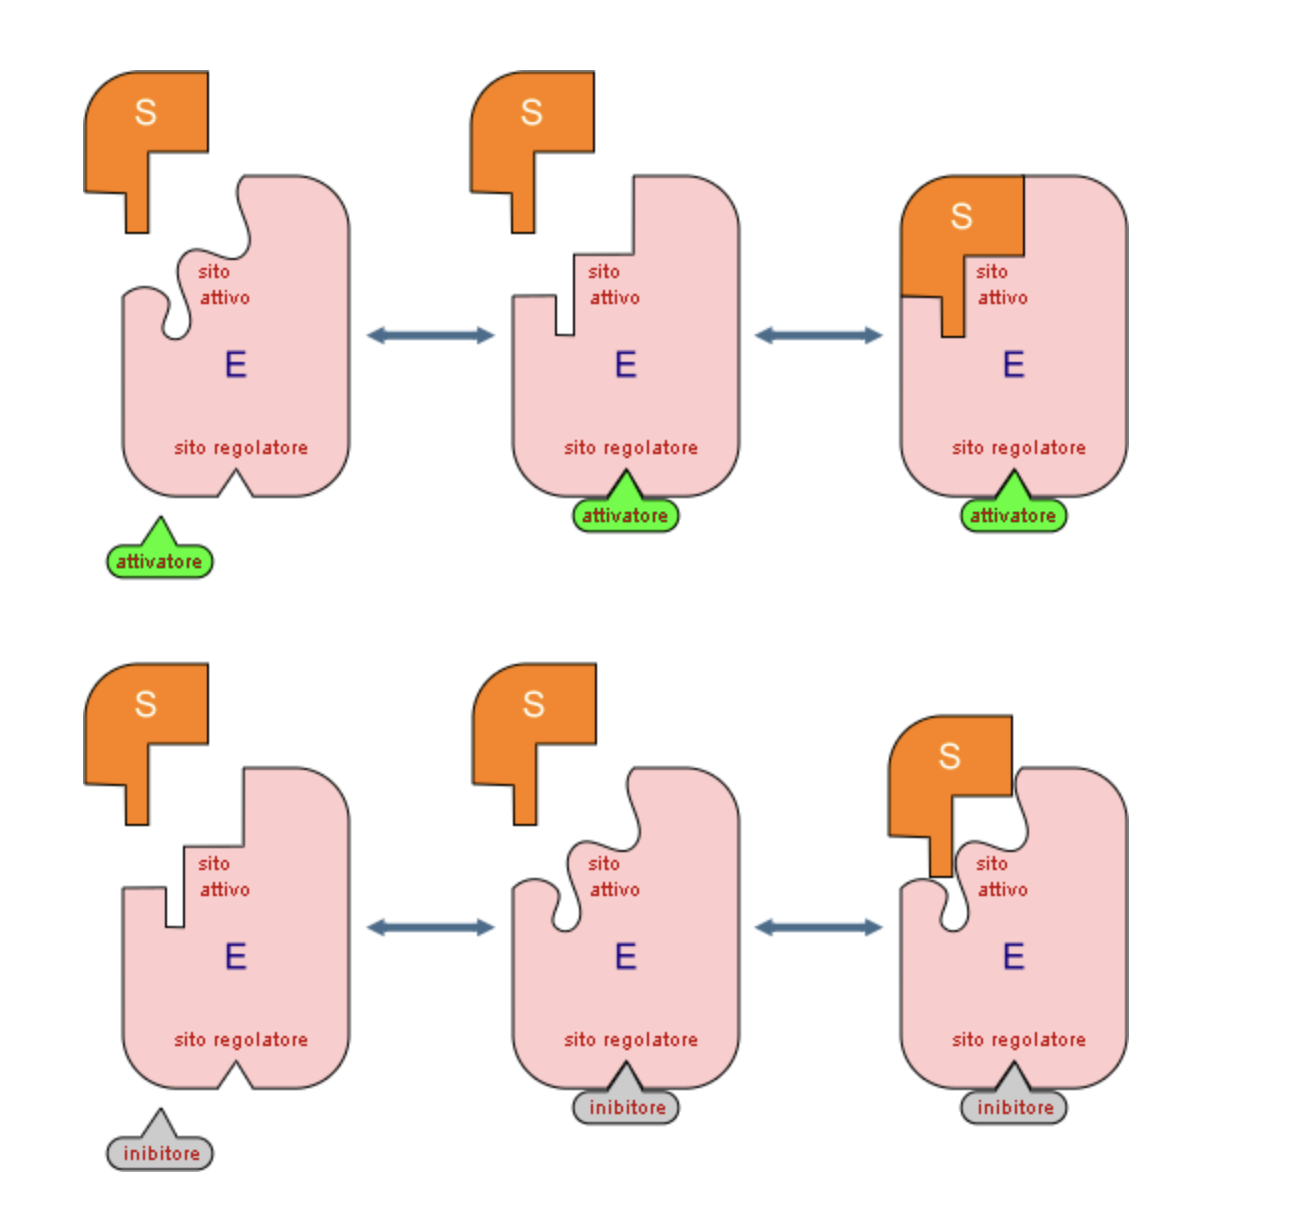
\includegraphics[width=1\textwidth]{/Users/enrico/PROTEINS/tesi/immagini_tesi_ingelse/Screenshot 2024-12-17 at 10.57.30.png}
    \caption{Schema of allosteric mechanism with active and allosteric site}
\end{figure}

\subsection{Thesis Structure}

\paragraph{Chapter 1: Protein Structure} \\
In the first chapter we will explain what a protein is and the basic concept about it.

\paragraph{Chapter 2: Relation structure-function-dynamic in proteins} \\
In the second chapter we will expose the importance relation structure-function-dynamic in proteins. 
It is very important the geometry structure of the protein and one of my aim is to show how much of the protein's behavior can be explained only from its geometric structure.
In fact it comes from years and years of evolutionary optimization process.

\paragraph{Chapter 3: Relation structure-function-dynamic in proteins} \\
In the third chapter we will study the normal modes and the guassian network model as a model to trehat the protein as a network of interactions between atoms.
This is a very useful model to study the protein's behavior and in particular the allosteric mechanism, in which model the geometric structure is the only important factor to explain the protein's behavior.
Finaly we will introduct the allosteric mechanism and we will see specifically in 3LNX protein, where we expect that a signal from an allosteric site can propagate to the hydrophobic pocket, that is the active site of the protein, avoiding the protein to catch a ligand.\\


\paragraph{Chapter 4: Causality indicators} \\
We will study also the causality indicators, that are a powerful tool to study the propagation of the signal along the protein's structure and to undestrand the allosteric mechanism.
We will present the covariace, the response and the transfer entropy as causal indicators.
\paragraph{Chapter 5: Causality indicators} \\
We will show the result and how good this model explain the allosteric behavior of the protein.

\vspace{1cm}








\chapter{Proteins}
\noindent Proteins are composed of a sequence of amino acids that fold into a three-dimensional structure that determines their function. \\
So proteins can have different types of functions, for example they can accelerate chemical reactions by reducing activation energy (Enzymatic catalysis), regulate cellular signal transduction and gene expression (Regulation and signaling), transport molecules across cellular membranes (Transport), provide mechanical support and structural integrity to tissues (Structural roles).\\
Our goal is to study the interactions between the amino acids that compose the protein, in particular we would like to understand allosteric mechanisms (as we will see in the next chapter).

\newpage
\section{Structure of amino acids}
\noindent For the fact that a protein is a sequence of amino acids we first need to understand what is an amino acid.\\
Amino acids are the building blocks of proteins, they are organic molecules that contain a central carbon atom (\(\alpha\)-carbon) bonded to an amino group (-NH2), a carboxyl group (-COOH), a (\(R\)-Group), that changes from amino acid to amino acid, and finally to a hidrogen atom\\
The \(R\)-group is particularly important because it determines the chemical properties of the amino acid, such as whether it is hydrophilic, hydrophobic, acidic, or basic.\\
\begin{figure}[H]
    \centering
    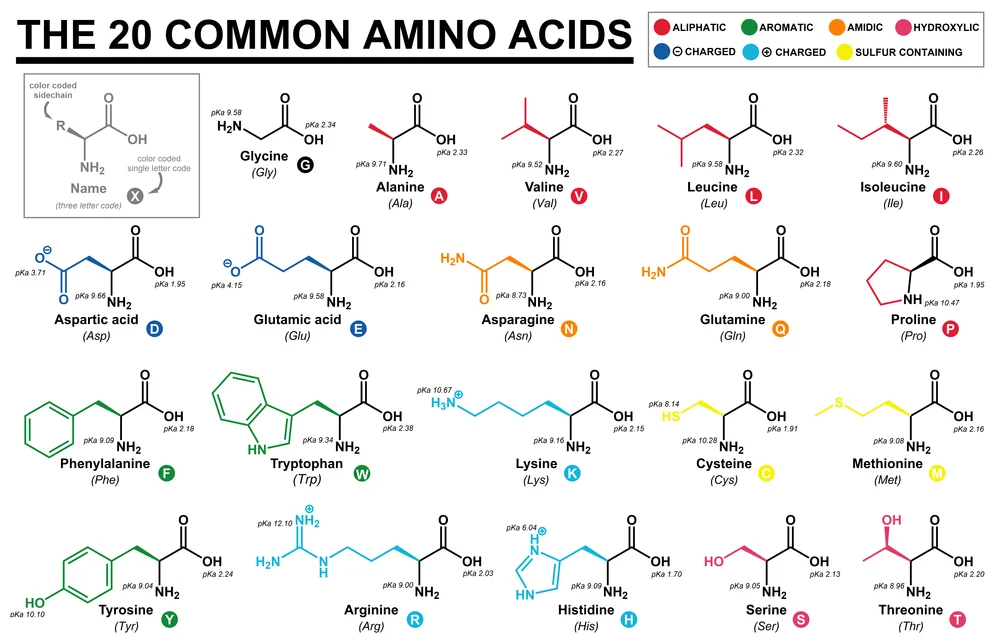
\includegraphics[width=1\textwidth]{/Users/enrico/PROTEINS/tesi/immagini_tesi_ingelse/ammino.png}
    \caption{Amino Acids}
\end{figure}
\newpage




\section{Protein structure}
\noindent 
The structure of a protein is divided into four levels which are very important for understanding its function:\cite{ref4}\\
The primary structure is a linear sequence of amino acids in a protein chain, held together by peptide bonds.\\ 
Instead the secondary structure represents the local folding of the protein chain in patterns.
In this work we will focus in the following secondary structures: alpha-helix, beta-sheet and loop. The first two are ordered patterns in which every amino acid is connected with the other amino acid in a specific way, the loop instead is a disordered region of the protein.\\
In particular alpha-helix is a right-handed spiral structure stabilized by hydrogen bonds between the NH and CO groups of amino acids separated by four residues, while beta-sheet is a structure in which the amino acids are connected by hydrogen bonds in a zigzag ( parallel or antiparallel) pattern
and finally the loop is a region of the polypeptide chain that connect other secondary structures.\\
The tertiary structure describes the three-dimensional folding of the entire protein molecule 
and quaternary structure consist of more than one polypeptide chain that are arranged and interact with each other to form the functional protein complex.
Obviously all these structures arise from the interactions between the amino acids that compose the protein. 
Following we will see our model for understanding the interaction between the amino acids.

\begin{figure}[H]
    \centering
    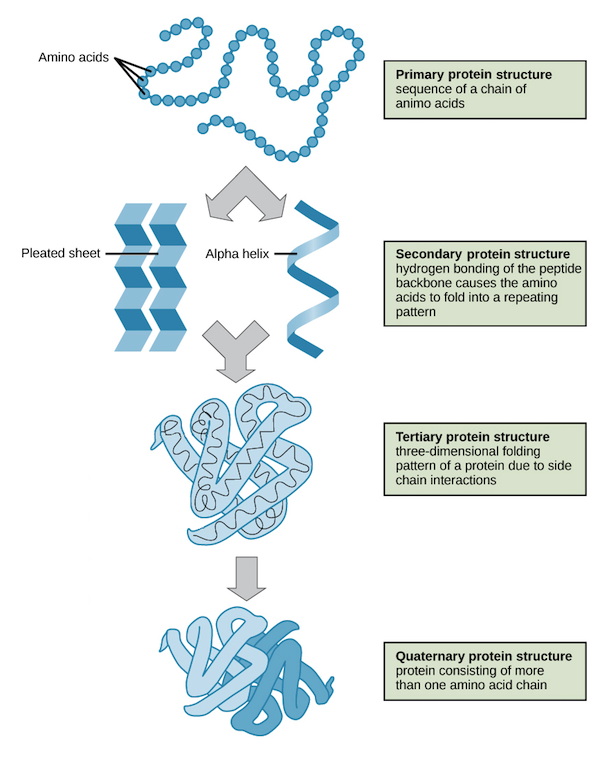
\includegraphics[width=0.5\textwidth]{/Users/enrico/PROTEINS/tesi/immagini_tesi_ingelse/71225d815cafcc09102504abdf4e10927283be98.png}
    \caption{Structures}
\end{figure}



\newpage

\chapter{Structure-Function-Dynamic Relationship in Proteins}


\section{Relation structure-function-dynamic in proteins}
\noindent The fundamental idea is that a protein's structure dictates its function. This structure governs the interactions between amino acids and proteins. If proteins were random aggregates of amino acids, they would not be able to perform their specific functions. Evolution optimizes the protein’s utility function, creating a structured arrangement that is not random.
This structure determines how the signal propagates along the protein.\\
Conformational flexibility in proteins is crucial for their function, as it allows transitions between different configurations. However, it is not just about oscillations around an equilibrium position: proteins often experience cooperative effects between distant regions, which are essential for complex biological activities such as ligand binding or interaction with other biomolecules.
To undergo a conformational changing protein can fluctuate, so its amino acids oscillate around an equilibrium position;
otherwise protein can linked with another amino acid and so it can change its conformation for example.\\
So we believe (and it is the entire supposition of this work) that only the factor about the geometry of the protein explains a lot about allosteric mechanism.
So we will do a model only dependent from the structure and we will try to explain everything. 
Obviously there are a lot of additional factors that we should add to model in the best way the behavior of a protein.\\

\newpage
\section{Allostery}

\noindent Allostery, derived from the Greek \textit{allos} (other) and \textit{stereos} (structure), is the phenomenon of a change in protein structure caused by the transmission of a signal from one site to another.\cite{ref5}  
More precisely, allostery occurs when the interaction of a molecule (effector) with a specific site on a protein, known as the allosteric site, induces a conformational change that influences the functional activity of another site, usually the active site. This process does not involve direct interactions between the two sites but occurs through changes in the protein’s internal network.

There are two key types of allostery that govern how proteins regulate their functions: conformational allostery and dynamic allostery. While both are based on the transmission of a signal through the protein’s structure, they differ in the mechanism of action.

\subsection{Conformational Allostery}  
\noindent Conformational allostery involves a structural change in the protein that occurs when an effector molecule binds to an allosteric site. This binding induces a distinct, often visible, shift in the protein’s shape, such as a transition from a less active (relaxed) state to a more active (tense) state. This structural shift propagates through the protein, modifying its function.

Mathematically, conformational allostery can be described in terms of the population of microstates of the protein, as well as the equilibrium constant between different states, such as:

\[
L = \frac{[T]}{[R]}
\]

where \([T]\) and \([R]\) represent the relative concentrations of the two conformational states, relaxed and tense, and \(L\) describes the equilibrium constant between them.

\begin{figure}[h]
    \centering
    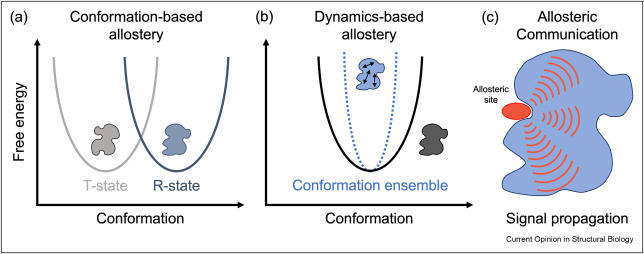
\includegraphics[width=\textwidth]{/Users/enrico/PROTEINS/tesi/immagini_tesi_ingelse/1-s2.0-S0959440X23002117-gr1.jpg}
    \caption{Schematic representation of allostery: the interaction with an allosteric effector (site A) induces a conformational change that affects a distant site (site B).}
    \label{fig:allostery_dynamics}
\end{figure}

\subsection{Dynamic Allostery}  
\noindent In contrast, dynamic allostery is based on fluctuations and flexibility within the protein’s structure. Instead of a fixed structural change, dynamic allostery involves the modulation of the protein’s internal dynamics, where small oscillations or fluctuations in the protein’s atomic structure propagate across its network of interactions. These dynamic changes influence the protein's ability to bind ligands or interact with other biomolecules.

Dynamic allostery often does not result in obvious structural shifts but involves subtle changes in the protein's flexibility. These changes are essential for the protein’s function, as they allow the protein to respond to environmental signals without requiring large-scale conformational changes.

\subsection{Causal Allostery: The Mechanisms of Signal Transmission}  
\noindent The propagation of signals within the protein can be understood as a causal mechanism that drives the allosteric response.\\
Both conformational and dynamic allostery rely on causal mechanisms—specifically, how an effector molecule's binding event at one site causes changes at a distant site. However, the distinction lies in how these signals are transmitted.\\
In conformational allostery, this is typically achieved through a direct structural change, while in dynamic allostery, it occurs via shifts in the protein's internal network dynamics, often without a distinct change in overall structure.\\
To fully grasp how proteins achieve their functional structure, it is crucial to explore the causal mechanisms behind these conformational and dynamic changes. Understanding how the signal propagates between amino acids and how localized binding events can influence distant regions of the protein is essential for studying allosteric mechanisms. This propagation of information is key to explaining how localized interactions can regulate the overall function of the protein, thus facilitating complex biological processes.
This understanding is especially important in drug development, where manipulating these allosteric sites and their causal mechanisms can lead to the creation of more effective therapeutic strategies.

\newpage

\subsection{Practical Example of Allostery: HIV Protease}  
\noindent The HIV protease is a key enzyme in the maturation of the HIV virus. After infecting a host cell, the virus produces a long chain of amino acids that must be cleaved into smaller peptides to form a functional, infectious protein. This process is regulated by allosteric mechanisms, where the binding of specific molecules to the protease induces conformational changes, affecting its ability to cleave the peptide chain and thus regulating viral maturation.

These cuts are essential for the virus to assemble the amino acids and mature into an infectious form. Therefore, inhibiting the protease's cutting ability can limit viral growth. This is exactly how protease inhibitors work in antiviral treatments.

This conformational change induced by allostery is a prime example of the importance of understanding allosteric mechanisms in proteins, as it enables us to intervene in processes crucial for viral replication and devise more effective treatments.

\begin{figure}[h]
    \centering
    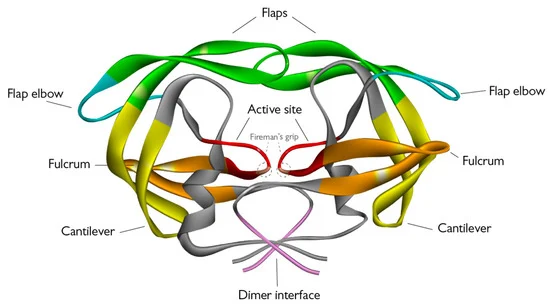
\includegraphics[width=\textwidth]{/Users/enrico/PROTEINS/tesi/immagini_tesi_ingelse/viruses-15-00712-g003-550.png}
    \caption{Structure of HIV Protease.}
    \label{fig:HIV}
\end{figure}



\newpage


\section{PDZ Domain}
\noindent 
In molecular biology, a domain is a specific region of a protein that can perform a structural or functional role independently from the rest of the protein.\cite{ref8} \\
They are tipycally characterized by two main characteristics; the first it is that the domain (as we said a portion of the protein) can fold into a three-dimensional structure on its own, the second is that it can play an indipendent role when it is unit with a protein.
In addition, because it is a modular unit, it is used by other proteins to form more complex structures.\cite{ref8} \\
Proteins often consist of multiple domains arranged in various combinations, creating multifunctional macromolecules capable of complex interactions. 


\subsection{The PDZ Domain}
\noindent The PDZ domain is a well-studied example of a protein domain. 
It is named after the three proteins in which it was first identified (Postsynaptic density protein 95,Drosophila discs large protein, Zona Occludens), it is a modular domain, its function is to organize and stabilize large multiprotein complexes, maintaining cellular architecture and facilitating biochemical signaling pathways. \cite{ref8}\\
The PDZ domain typically consists of 80--90 amino acid; facilitates protein-protein interactions by recognizing specific peptide sequences, often located at the C-terminal region of target proteins; assemble protein complexes at cellular membranes


\subsection{The PDZ Domain in the 3LNX Protein and its structure}

\noindent The 3LNX protein offers important insights into the functioning of these domains.\\
This protein has a hydrophobic pocket that accommodates a external peptide, that binds with the 3LNX.\\
It is constitute from three alpha helix, that we will call alpha-$\alpha$, alpha-$\beta$ and $alpha-\gamma$, and six different beta-sheet, that we will call beta-$\alpha$, beta-$\beta$, $beta-\gamma$,$beta-\delta$, $beta-\epsilon$,$beta-\eta$. \\
\begin{figure}[H]
    \centering
    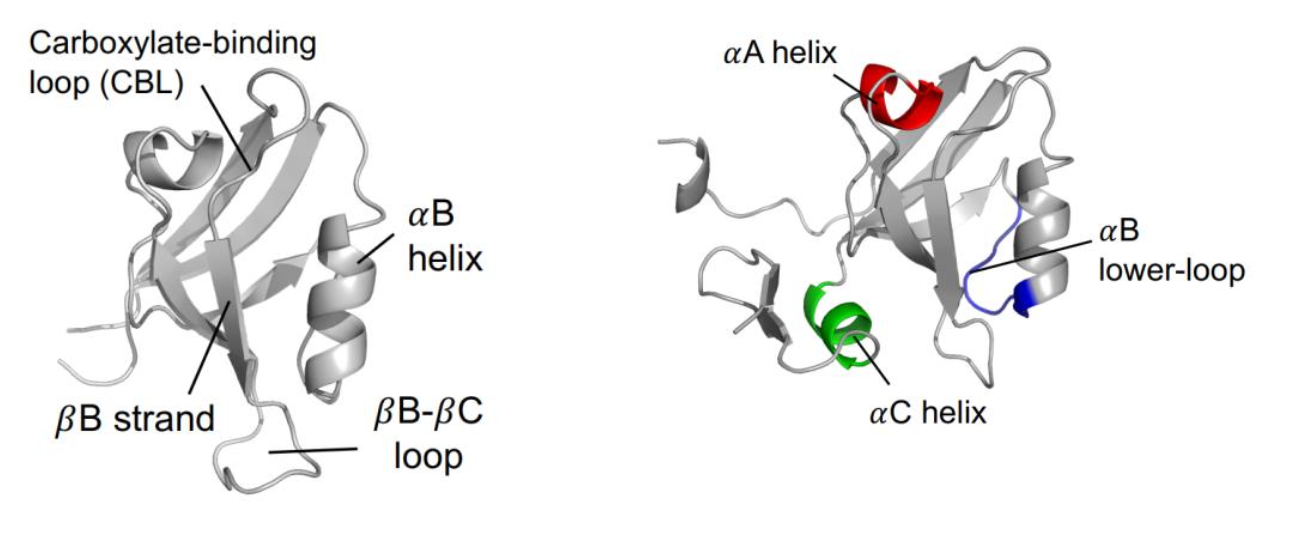
\includegraphics[width=1\textwidth]{/Users/enrico/PROTEINS/tesi/immagini_tesi_ingelse/Screenshot 2024-12-17 at 08.59.09.png}
    \caption{3LNX protein}
\end{figure}
The allosteric mechanism works as follows: a perturbation at one allosteric site propagates a signal towards the hydrophobic pocket, located between the $\beta$-sheet and the $\alpha$-helix. \\
This pocket can transition between open and closed states, which is the essence of allostery, preventing a ligand from binding or unbinding at the active site within the hydrophobic pocket. \\
These allosteric sites do not directly interact with the ligand but are crucial for transmitting structural changes within the protein upon ligand binding. In this study, we will investigate in detail two potential allosteric sites, identified by experimental biologists, located in the $\alpha$-helix and the $\gamma$-helix, as suggested by previous research. \cite{ref15}.\\
So this is the schema of what we expect:


\begin{tikzpicture}[node distance=2cm]

    % Nodes for perturbation and regions
    \node (alphaalpha) [draw, rectangle, text centered, minimum height=1cm, minimum width=2cm] {alpha-$\alpha$ helix};
    \node (alphabeta) [draw, rectangle, text centered, minimum height=1cm, minimum width=2cm, right=of alphaalpha] {alpha-$\gamma$ helix};
    
    % Nodes for regions below alpha-alpha and alpha-gamma, aligned horizontally
    \node (bindingAlphaAlpha) [below of=alphaalpha, draw, rectangle, text centered, minimum height=1cm, minimum width=2.5cm, yshift=-1cm] {Binding Pocket};
    \node (bindingAlphaGamma) [below of=alphabeta, draw, rectangle, text centered, minimum height=1cm, minimum width=2.5cm, yshift=-1cm] {Binding Pocket};
    
    % Draw arrows from alpha-alpha and alpha-gamma to each region
    \draw[->] (alphaalpha) -- (bindingAlphaAlpha);
    \draw[->] (alphabeta) -- (bindingAlphaGamma);

\end{tikzpicture}







\newpage
\chapter{Normal and functional mode Analysis}
\section{Introduction}
\noindent 
Normal Mode Analysis (NMA) is a technique that allows to descibe a system in term of normal modes. These are a quantitative method to express the vibration intensity of every atom that constitutes the system.
The normal modes are collective and can be low or high frequency motions. They come from an harmonic (gaussian) approximation of the system.


\section{Structure--Function--Dynamics Relationship}
\noindent 
Proteins are thermodynamical entities (infact they are immersed in a fluid) that costantly fluctuate around an equilibrium energetic landscape.
This normal mode describe very well the vibrations of each atoms around their equilibrium points. With this tecnique i can identify the modes and the most important sites for allosteric's mechanisms.
Thus, NMA provides a link between structure, function, and dynamics;
infact starting from geometrical structure of the protein we can compute the normal modes and we can use them to study the allostery into the proteins.
So NMA offers a theoretical bridge between the structure and the funciton of a protein.


\section{Introduction to Normal Modes and Their Physical Significance in Proteins}
\noindent As we said normal modes are a powerful tools for understanding protein dynamics. \\
They are derived from the diagonalization of the Hessian matrix \eqref{hessian} of the hamiltonian, \( \mathbf{H} \)
which encapsulates the curvature of the potential energy surface near a local minimum. 
Mathematically normal modes are the eigenvectors \( \mathbf{v}_k \) of the Hessian matrix. 

For every eigenvectors i have an associated eigenvalue \( \lambda_k \) which is proportional to the squared frequencies of these motions (as we will see in few lines):

\begin{equation}
\mathbf{H} \mathbf{v}_k = \lambda_k \mathbf{v}_k. \label{equazione}
\end{equation}

For understanding where that come from, we need to consider the Taylor expansion of the potential energy \( V(\mathbf{x}) \) around a minimum point \( \mathbf{x}_0 \):

\begin{equation}
V(\mathbf{x}) \approx V_0 + \frac{1}{2} \mathbf{x}^T \mathbf{H} \mathbf{x},
\end{equation}

where \( V_0 \) is the potential energy at the minimum, and \( \mathbf{x} \) represents the displacement from equilibrium. This quadratic, so a gaussian, approximation that assumes small displacements, making the system effectively harmonic.
We can write the motion's equation using the hamiltonian (constitute only from the potential energy) , in fact the force \( \mathbf{F} \) is minus the gradient of the potential energy:

\begin{equation}
\mathbf{F} = -\nabla V(\mathbf{x}) = -\mathbf{H} \mathbf{x}.
\end{equation}

So i have:

\begin{equation}
\mathbf{M} \ddot{\mathbf{x}} = -\mathbf{H} \mathbf{x},
\end{equation}
where \( \mathbf{M} \) is the diagonal mass matrix.

Now we normalize the coordinates with a change of variable: \( \mathbf{x}' = \sqrt{M} \mathbf{x}\). \\
So substituting this transformation we obtain:

\begin{equation}
\ddot{\mathbf{x}} = -\mathbf{H} \mathbf{x}.
\end{equation}
The solution of this equation is of the form \( \mathbf{x}(t) = \mathbf{v}_k e^{i \omega_k t} \), where \( \omega_k \) is the angular frequency of the \( k \)-th mode and \( \mathbf{v}_k \) is the corresponding eigenvector. Substituting this into the equation of motion:

\begin{equation}
-\omega_k^2 \mathbf{v}_k = -\mathbf{H} \mathbf{v}_k.
\end{equation}

This equation demonstrates that \( \lambda_k \), the k-th eigenvalue of the Hessian, is related to the angular frequency by, as equation \ref{equazione}:

\begin{equation}
\omega_k^2 = \lambda_k.
\end{equation}

Taking the square root, the normal mode frequencies are given by:

\begin{equation}
\omega_k = \sqrt{\lambda_k}.
\end{equation}

The interpretation of that is that the eigenvectors \( \mathbf{v}_k \) tell us the directions of motion in the space of atomic coordinates and every mode represent a distinct oscillation of every atoms of the protein.\\
In addition the low intensity values of eigenvalues correspond to low frequency modes are usually in literature associate with long range effect and high frequency oscillationa re associated with local effects.
Typically the long range modes are assocaited with functions like the opening and closing of ligand-binding sites which are  allosteric transitions, 


\newpage



\section{Gaussian Network Model}
\noindent
Let's start to model our protein.\\ First we need a Hamiltonian to describe the system:
If the protein is at equilibrium, we expect that the Hamiltonian is a function of a potential that depends on the position of every atom constituting the PDZ-specific domain, from bonding forces between atoms, electrostatic and Van Der Walls interactions, solvent forces and from a lot of additional factors.\\
As it clear it is very complex to develop a real world model in this field, but it is not our goal. Our aim is to understand how much of this physical system is explainable only from its geometric.\\
In this model, we represent the Hamiltonian of the system as H=V(r) where r is the vector containing the positions of all the atoms that make up the protein. This approach is based on the assumption that the protein’s dynamics can be effectively described using only its geometric structure, specifically focusing on the positions of the backbone atoms (alpha-carbons), while neglecting finer details such as side-chain interactions or solvent effects.\\
While this simplification allows for manageable computational complexity, it may overlook important local and long-range interactions.
Due to the complexity of the system, it is not feasible to solve it exactly. Therefore, we rely on approximations, such as the second-order expansion of the potential energy around an equilibrium point, which provides a simplified representation of the protein's behavior. However, this approximation neglects higher-order interactions that could influence the protein’s dynamics, and as a result, it may fail to capture certain intricate behaviors, especially in regions where the protein undergoes significant conformational changes.
The second-order approximation of a function \( V(\mathbf{r}) \), around an equilibrium point \( \mathbf{r}_0 \), can be expressed as:\cite{ref9}

\begin{equation}
V(\mathbf{r}) \approx V(\mathbf{r}_0) + \nabla V(\mathbf{r}_0)^\top (\mathbf{r} - \mathbf{r}_0) + \frac{1}{2} (\mathbf{r} - \mathbf{r}_0)^\top \mathbf{H_V} (\mathbf{r} - \mathbf{r}_0),\label{hessian}
\end{equation}

where:
\begin{itemize}
    \item \( V(\mathbf{r}_0) \) is the value of the function at the equilibrium point \( \mathbf{r}_0 \).
    \item \( \nabla V(\mathbf{r}_0) \) is the gradient of the function, defined as:
    \begin{equation}
    \nabla V(\mathbf{r}) = \frac{\partial V}{\partial \mathbf{r}} \bigg|_{\mathbf{r} = \mathbf{r}_0},
    \end{equation}
    which equals zero if \( \mathbf{r}_0 \) represents a minimum point, corresponding to the equilibrium position.
    \item \( \mathbf{H_V} \) is the \textbf{Hessian matrix} of \( V(\mathbf{r}) \), defined as:
    \begin{equation}
    \mathbf{H_V} = \frac{\partial^2 V}{\partial \mathbf{r}^2} \bigg|_{\mathbf{r} = \mathbf{r}_0},
    \end{equation}
    \[
    \mathbf{H} = \begin{bmatrix}
    \frac{\partial^2 V}{\partial x_1^2} & \frac{\partial^2 V}{\partial x_1 \partial x_2} & \cdots & \frac{\partial^2 V}{\partial x_1 \partial x_{3N}} \\
    \frac{\partial^2 V}{\partial x_2 \partial x_1} & \frac{\partial^2 V}{\partial x_2^2} & \cdots & \frac{\partial^2 V}{\partial x_2 \partial x_{3N}} \\
    \vdots & \vdots & \ddots & \vdots \\
    \frac{\partial^2 V}{\partial x_{3N} \partial x_1} & \frac{\partial^2 V}{\partial x_{3N} \partial x_2} & \cdots & \frac{\partial^2 V}{\partial x_{3N}^2}
    \end{bmatrix}.
    \]
    It is a symmetric matrix that describes the curvature of \( V(\mathbf{r}) \) around \( \mathbf{r}_0 \).
\end{itemize}

It is important to note that the \textbf{Hessian matrix} \( \mathbf{H_V} \) should not be confused with the \textbf{Hamiltonian}, which represents the total energy of a system.  

Thus, apart from constants, the Hamiltonian can be approximated as:
\begin{equation}
V(\mathbf{r}) \approx \frac{1}{2} (\mathbf{r} - \mathbf{r}_0)^\top \mathbf{H_V} (\mathbf{r} - \mathbf{r}_0). \label{1.1}
\end{equation}
This modeling is called Gaussian Network Model (GNM) and is commonly used to study the dynamic of proteins.\\
To reduce the computational complexity of the proble  we will focus solely on the \(\alpha\)-carbon atoms because they form the backbone of the protein and their positions are sufficient to reconstruct the global three-dimensional conformation of the protein.
This model is overall extendable to all other atoms of the protein without a lot of difficulty.\\
So to summarize this is a model which take in consideration only the geometric structure of the protein and no one of the other type of interactions. So it will explain only the effects and allosteric mechanism due to structure.
\newpage



\section{Interpretation of the Taylor Expansion}
\noindent Equation \eqref{1.1} can be interpreted not only as the Hamiltonian of the harmonic oscillator (spring-system) but also as a network model, where every \(\alpha\)-carbon atom is a node interacting with other nodes.\cite{ref9}

\subsubsection{Definition of a Graph}
\noindent 
A graph \( G \) is a mathematical structure used to model pairwise relations between objects.\\ It consists of a set of vertices \( V \) (also called nodes) and a set of edges \( E \), where each edge connects a pair of vertices.
Graphs can be directed or undirected, weighted or unweighted, depending on the nature of the relationships they represent.\cite{ref11}\\

\begin{figure}[h]
    \centering
    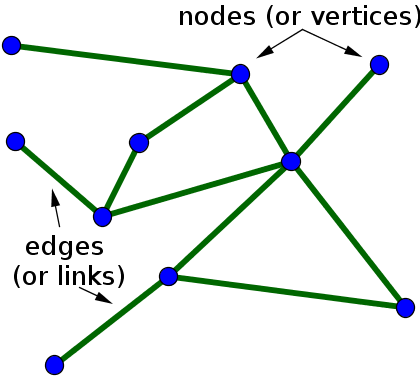
\includegraphics[width=\textwidth]{/Users/enrico/PROTEINS/tesi/immagini_tesi_ingelse/small_undirected_network_labeled-2.png}

    \caption{Schematic representation of a Network.}
    \label{fig:Network}
\end{figure}

\subsubsection{Kirchhoff Matrix (Laplacian Matrix)}
\noindent The Kirchhoff matrix is a matrix that represent the connection between nodes in a graph, avoiding to encode informations about its structure.\\
For a graph \( G \) with \( n \) vertices, the Laplacian matrix \( L \) is defined as:\cite{ref11}
\begin{equation}
    L = D - A \label{Kirchhoff}
\end{equation}
Where \( D \) is the degree matrix, a diagonal matrix defined as:
\begin{equation}
    D_{ij} = 
    \begin{cases} 
      \deg(v_i) & \text{if } i = j, \\
      0 & \text{if } i \neq j,
    \end{cases}
\end{equation}
where \( \deg(v_i) \) is the degree of vertex \( v_i \), the number of edges connected to vertex (nodes) \( i \);  and \( A \) is the adjacency matrix, a square matrix defined as:
\begin{equation}
    A_{ij} = 
    \begin{cases} 
      1 & \text{if there is an edge between vertices } v_i \text{ and } v_j, \\
      0 & \text{otherwise}.
    \end{cases}
\end{equation}

By the property of simmetry of \( L \)  it follows that it is diagonalizable, it is positive semi-definiteness, and its smallest eigenvalue is always 0.
Causa it is semidefinite positive we can't have the inverse but we can obtain the pseudo-inverse which is the matrix \( L^+ \) that minimize the following equation: 
\[
L^+ L = L L^+ = I - \frac{1}{n} \mathbf{1} \mathbf{1}^\top
\]
where \( n \) is the number of nodes and \( \mathbf{1} \) is a vector of all ones.




\newpage
\section{Gaussian Network Model (GNM)}
\noindent Now that i know what the Kirchoff matrix is we can express the Hamiltonian of the system, following \eqref{1.1}, as:\cite{ref12}
\begin{equation}
    H(\mathbf{r}) \approx \frac{1}{2} (\mathbf{r} - \mathbf{r}_0)^\top \mathbf{K} (\mathbf{r} - \mathbf{r}_0),
\end{equation}
where \( \mathbf{K} \) is the Laplacian matrix. For simplicity, we can rewrite it as:
\begin{equation}
    H(\mathbf{r}) \approx \frac{1}{2} \mathbf{r}^\top \mathbf{K} \mathbf{r},
\end{equation}
or, in components:
\begin{equation}
    H(\mathbf{r}) \approx \frac{1}{2} \sum_{i,j} r_i K_{ij} r_j.
\end{equation}
Here, \(\mathbf{r}\) represents the displacement vector of atoms from their equilibrium positions.\\
For simplicity we can assume isotropy and from now \(\mathbf{r}\) will be one dimensional.

From this simple formulation of the system we can derive some statistical properties.

Initially, the probability density at equilibrium is given by:\cite{ref12}
\begin{equation}
    P(\mathbf{r}) = \frac{1}{Z} e^{-\beta H(\mathbf{r})},
\end{equation}
where the partition function \(Z\) is:
\begin{equation}
    Z = \int e^{-\beta H(\mathbf{r})} \, d\mathbf{r}.
\end{equation}

Defined it i can derive a lot of information in addition of my system like:

\subsubsection{Mean displacement}
\noindent The mean position \(\langle \mathbf{r} \rangle\) can be calculated as:\cite{ref12}
\begin{equation}
    \langle \mathbf{r} \rangle = \int \mathbf{r} P(\mathbf{r}) \, d\mathbf{r},
\end{equation}
where:
\begin{equation}
    P(\mathbf{r}) = \frac{1}{Z} e^{-\frac{\beta}{2} \mathbf{r}^\top \mathbf{K} \mathbf{r}},
\end{equation}
and the partition function is:\cite{ref12}
\begin{equation}
    Z = \int e^{-\frac{\beta}{2} \mathbf{r}^\top \mathbf{K} \mathbf{r}} \, d\mathbf{r}.
\end{equation}

Substituting \(P(\mathbf{r})\) into the expression for \(\langle \mathbf{r} \rangle\), we obtain:
\begin{equation}
    \langle \mathbf{r} \rangle = \frac{1}{Z} \int \mathbf{r} e^{-\frac{\beta}{2} \mathbf{r}^\top \mathbf{K} \mathbf{r}} \, d\mathbf{r}.
\end{equation}

Since the integrand \(\mathbf{r} e^{-\frac{\beta}{2} \mathbf{r}^\top \mathbf{K} \mathbf{r}}\) is symmetric with respect to \(\mathbf{r}\), and there are no linear terms in the Hamiltonian, the Gaussian distribution is centered at \(\mathbf{r} = 0\). Therefore:\cite{ref12}
\begin{equation}
    \langle \mathbf{r} \rangle = 0.
\end{equation}

\subsubsection{Covariance}
\noindent The covariance between \(r_i\) and \(r_j\) is defined as:\cite{ref12}
\begin{equation}
    \text{Cov}(r_i, r_j) = \langle r_i r_j \rangle - \langle r_i \rangle \langle r_j \rangle.
\end{equation}

Since \(\langle r_i \rangle = 0\), it simplifies to:
\begin{equation}
    \text{Cov}(r_i, r_j) = \langle r_i r_j \rangle.
\end{equation}

Using the Boltzmann distribution:
\begin{equation}
    P(\mathbf{r}) = \frac{1}{Z} e^{-\frac{\beta}{2} \mathbf{r}^\top \mathbf{K} \mathbf{r}},
\end{equation}
we calculate:
\begin{equation}
    \langle r_i r_j \rangle = \frac{1}{Z} \int r_i r_j e^{-\frac{\beta}{2} \mathbf{r}^\top \mathbf{K} \mathbf{r}} \, d\mathbf{r}.
\end{equation}

For a Gaussian distribution, the covariance matrix is given by:
\begin{equation}
    \bm{\Sigma} = \beta^{-1} \mathbf{K}^{-1} = \langle r_i r_j \rangle,
\end{equation}
where \((\mathbf{K}^{-1})_{ij}\) represents the \((i,j)\)-th element of \(\mathbf{K}^{-1}\). Thus:
\begin{equation}
    \text{Cov}(r_i, r_j) = \frac{1}{\beta} (\mathbf{K}^{-1})_{ij}.
\end{equation}

\subsection{Derivation of diffraction intensity with atomic vibrations}
\noindent The diffraction intensity in crystallography and biology is influenced by the atomic vibrations around their mean positions.\\
These vibrations are characterized by the mean squared displacement, denoted as $\langle r^2 \rangle$.
The thermal motion leads to a modification of the scattering factor:
\[
f(\mathbf{q}) = f_0(\mathbf{q}) \cdot e^{-2\pi i \mathbf{q} \cdot \mathbf{u}}
\]
where $f_0(\mathbf{q})$ is thescattering factor for a stationary atom, $\mathbf{q}$ is the scattering vector and $\mathbf{u}$ is the displacement from the mean position.


The observed intensity $I(\mathbf{q})$ is proportional to the squared magnitude of the structure factor $F(\mathbf{q})$:
\[
I(\mathbf{q}) \propto |F(\mathbf{q})|^2 e^{-8\pi^2 \langle r^2 \rangle |\mathbf{q}|^2}.
\]

The factor $B = 8\pi^2 \langle r^2 \rangle$ emerges naturally, leading to:
\[
I(\mathbf{q}) \propto |F(\mathbf{q})|^2 e^{-B |\mathbf{q}|^2}.
\]
This factor $B$ is called beta-factor and i can write it as a function of covaricne/variance:
$B_i = 8\pi^2 \langle C_{i,i} \rangle$ 

This is an important metric in biology and in crystallographic because it describe how much disorder there is in the protein and for evaluating the model.


\section{Model Evaluation: RMSE and MAE }\label{sec:Evaluation}
Some of common metrics to evaluate a model are the RMSE and the MAE. 
\subsection{RMSE: Root Mean Square Error}
\noindent The formula for RMSE is:
\[
\text{RMSE} = \sqrt{\frac{1}{n} \sum_{i=1}^n (y_i - \hat{y}_i)^2}
\]
Where \(y_i\) are observed values, \(\hat{y}_i\) are predicted values.

\subsection{MAE: Mean Absolute Error}
\noindent The formula for MAE is:
\[
\text{MAE} = \frac{1}{n} \sum_{i=1}^n |y_i - \hat{y}_i|
\]
Where as before \(y_i\) are observed values, \(\hat{y}_i\) are predicted values.


\newpage

\section{Stochastic Processes}  \label{sec:stochastic_processes}
A stochastic process is a mathematical framework used to describe systems that evolve over time in a probabilistic manner.\\
We will use this mathematical tool to model the oscillation around the equilibrium position of each atom which constitutes the protein.\\
Such processes are essential in modeling phenomena in physics, biology, finance, and many other fields, where uncertainty and noise play significant roles.
In general, the evolution of termodinamical system can be expressed as:
\begin{equation}
    \gamma\frac{dX_t}{dt} = -\nabla H(X_t) + \sqrt{2 \gamma k_B T} \eta_t,
\end{equation}
where \( X_t \) represents the state of the system at time \( t \), \( H(X_t) \) is the Hamiltonian function, which dictates the deterministic behavior, \( \nabla H(X_t) \) is the gradient of the Hamiltonian, the force, describing the deterministic direction of motion, \( \nabla H(X_t) \) is the gradient of the Hamiltonian, the force, describing the deterministic direction of motion, \( \eta_t \) is a stochastic noise term, modeled as Gaussian white noise with zero mean and variance \( \sigma^2 \),  \( \langle \eta_t \eta_{t'} \rangle = \sigma^2 \delta(t-t') \), \( \gamma \) is the friction coefficient, which represents the dissipative interaction with the environment, \( k_B \) is the Boltzmann constant, a fundamental physical constant relating temperature and energy, is the Boltzmann constant and finally \( T \) is the temperature of environment,.
For simplicity, we set \( \gamma = 1 \, \text{s}^{-1} \), \( k_B = 0.5 \, \text{J/K} \), and \( T = 1 \, \text{K} \).
So it becomes:
\begin{equation}
    \frac{dX_t}{dt} = -\nabla H(X_t) + \eta_t,
\end{equation}
Now substituting the gradient into the general stochastic equation, using \eqref{1.1} we obtain:
\begin{equation}
\frac{d\mathbf{r}_t}{dt} = -\mathbf{K} \mathbf{r}_t + \boldsymbol{\eta}_t,
\end{equation}
where \( \mathbf{r}_t \) is the state vector at time \( t \), \( -\mathbf{K} \mathbf{r}_t \) is the deterministic term driving the system towards equilibrium, \( \boldsymbol{\eta}_t \) is a vector of independent Gaussian noise components.\\
Otherwise we can express it also in component form:
\begin{equation}
    \frac{d r_{i,t}}{dt} = -\sum_j K_{ij} r_{j,t} + \eta_{i,t}.
\end{equation}
The described dynamics correspond to a multidimensional Ornstein-Uhlenbeck process, which is the simplest continuous-time Gaussian process with a mean-reverting property.\\
Since \(\mathbf{K}\) is symmetric, it can be diagonalized:
\[
\mathbf{K} = \mathbf{U} \boldsymbol{\Lambda} \mathbf{U}^\dagger,
\]
where  \(\mathbf{U}\) is the orthogonal matrix of eigenvectors (\(\mathbf{U}^\dagger = \mathbf{U}^{-1}\)) and \(\boldsymbol{\Lambda} = \text{diag}(\lambda_1, \lambda_2, \dots, \lambda_N)\) is the diagonal matrix of eigenvalues.\\
By changing variables to the eigenbasis:
\[
\tilde{\mathbf{r}}(t) = \mathbf{U}^\dagger \mathbf{r}(t),
\]
the equation becomes:
\[
\frac{d \tilde{\mathbf{r}}(t)}{dt} = -\boldsymbol{\Lambda} \tilde{\mathbf{r}}(t) + \tilde{\boldsymbol{\eta}}(t),
\]
where \(\tilde{\boldsymbol{\eta}}(t) = \mathbf{U}^\dagger \boldsymbol{\eta}(t)\).\\
Since the transformation is orthogonal, \(\tilde{\boldsymbol{\eta}}(t)\) remains Gaussian white noise with the same properties as \(\boldsymbol{\eta}(t)\).

The diagonalization decouples the system into independent equations for each mode \(k\):
\[
\frac{d \tilde{r}_k(t)}{dt} = -\lambda_k \tilde{r}_k(t) + \tilde{\eta}_k(t),
\]
where \(\tilde{r}_k(t)\) is the \(k\)-th component of \(\tilde{\mathbf{r}}(t)\), \(\lambda_k\) is the \(k\)-th eigenvalue, and \(\tilde{\eta}_k(t)\) is the \(k\)-th component of the transformed noise.

The solution to the Ornstein-Uhlenbeck equation for each mode is:
\[
\tilde{r}_k(t) = \tilde{r}_k(0) e^{-\lambda_k t} + \int_0^t e^{-\lambda_k (t-s)} \tilde{\eta}_k(s) \, ds.
\]
Returning to the original variables:
\[
\mathbf{r}(t) = \mathbf{U} \tilde{\mathbf{r}}(t),
\]
we can write the solution as:
\[
\mathbf{r}(t) = \mathbf{U} \left[ \tilde{\mathbf{r}}(0) e^{-\boldsymbol{\Lambda} t} + \int_0^t e^{-\boldsymbol{\Lambda} (t-s)} \tilde{\boldsymbol{\eta}}(s) \, ds \right].
\]










































\newpage
\chapter{Introduction to causality and causality in allosteric mechanisms of proteins}
\noindent Our primary aim, as we just said, is to identify  the allosteric propagation of the signal from allosteric sites to other sites of the protein.\\
To understand the propagation of the signal we need to have a cause (the sorgent of the signal, in our case the allosteric site) and an effect (the dynamical changing in the protein).\\
So we need a causal mechanism e we have to indagate it; to reveal causality we saw only one useful indicator: the covariance/correlation.\\
But we know that correlation does not imply causation, so in the following pages we will discover new causal indicators.

\begin{figure}[h]
    \centering
    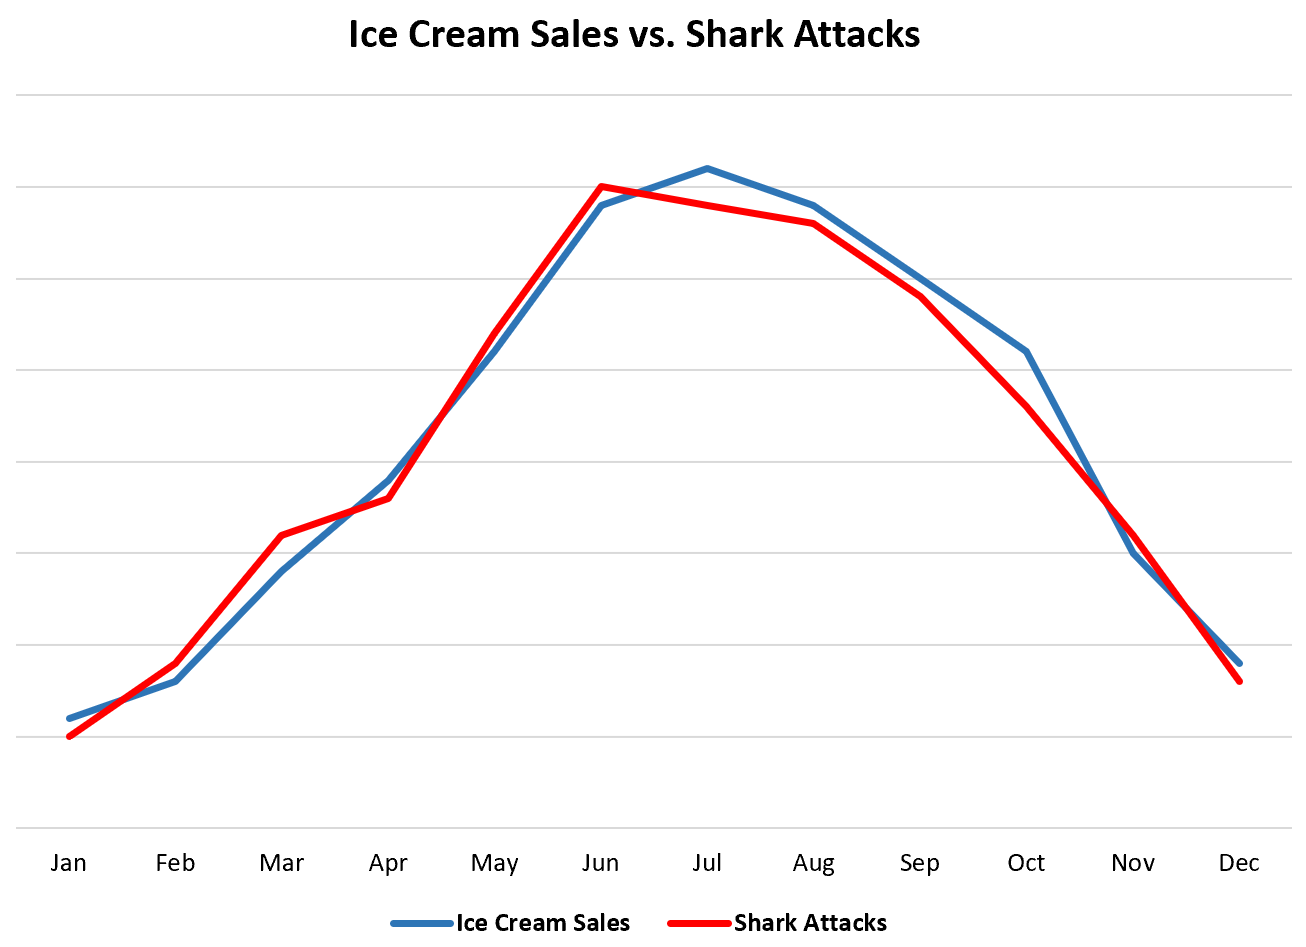
\includegraphics[width=\textwidth]{/Users/enrico/PROTEINS/tesi/immagini_tesi_ingelse/corrCause1.png}    
    \caption{Correlation is not causation.}
    \label{fig:Correlation is not causation}
\end{figure}


\newpage
\section{Deterministic and Stochastic Causality}
\noindent Causality refers to the relationship between causes and effects, where one event (the cause) directly influences or produces another event (the effect), so it implies a directional influence.
Mathematically causal relationships are often modeled as:\cite{ref14}
\[
B = f(A, \text{other factors}),
\]
where \( f \) describes how \( A \) and other factors jointly determine \( B \). 


Causality can be classified into two main types: deterministic and stochastic.

\subsection{Deterministic Causality}

\noindent Deterministic causality implies that a specific cause invariably leads to a specific effect. If an event \( A \) causes an event \( B \), then \( B \) always occurs whenever \( A \) occurs. \\
This relationship can be expressed as \( A \implies B \), meaning \( A \) is both necessary and sufficient for \( B \). \\
Deterministic causality is observed in systems governed by precise physical laws, such as classical mechanics, where given initial conditions and forces, trajectories are entirely predictable.

\subsection{Stochastic Causality}

\noindent Stochastic causality acknowledges that many causal relationships are probabilistic rather than absolute. 
Here, the occurrence of \( A \) increases the likelihood of \( B \), but \( B \) does not always follow \( A \). \\
This is expressed probabilistically as \( P(B|A) > P(B|\neg A) \), indicating that \( A \) raises the probability of \( B \). \\
Stochastic causality is prevalent in complex systems like biology or social sciences, where multiple interacting factors and inherent randomness influence outcomes. 
For example, smoking increases the probability of lung cancer, though not all smokers develop the disease.

\subsection{Causality and the Shannon Entropy}
\noindent This idea relates to Shannon entropy, defined as:
\[
H(X) = -\sum_{i} P(x_i) \log P(x_i),
\]
where \( X \) is a random variable with possible states \( x_i \), and \( P(x_i) \) is the probability of \( x_i \).\\
 When \( P(x_i) = \delta(x_i) \) -> \( H(X) = 0 \), the system has no uncertainty, indicating complete predictability.\\
So if my target variable has the distribution of the delta function, the entropy is zero, so the system is deterministic.\\
So the distribution width of the \( x_i \) determines how much my system is predictable. 
We will use this concept later.



\newpage
\section{Correlation}
\subsection{Correlation Between Fluctuations}
\noindent
The correlation between two variables, such as the fluctuations in the positions of particles \( i \) and \( j \), provides insight into how these components of the system interact.\\
The correlation function is defined as:\cite{ref13}
\begin{equation}
    C_{ij} = \langle \delta \mathbf{r}_i \cdot \delta \mathbf{r}_j \rangle, \label{correlation}
\end{equation}
where \( \delta \mathbf{r}_i = \mathbf{r}_i - \langle \mathbf{r}_i \rangle \) is the deviation of the position of particle \( i \) from its equilibrium value and \( \langle \cdot \rangle \) denotes an ensemble average.\\
The correlation \( C_{ij} \) quantifies the degree to which the positions of particles \( i \) and \( j \) are linearly related at equilibrium.\\
The correlation \( C_{ij} \) reflects how strongly two particles are connected in the system; if we have a positive correlation it indicates that fluctuations in \( \mathbf{r}_i \) and \( \mathbf{r}_j \) tend to occur in the same direction, suggesting cooperative behavior or a direct connection, if it is negative so fluctuations in \( \mathbf{r}_i \) and \( \mathbf{r}_j \) tend to occur in opposite direction, and finally a correlation of 0 indicates no linear relationship between the fluctuations, suggesting either independence or non-linear interactions.\\

\subsection{Why Correlation Alone is Not Causation}
\noindent While correlations reveal interactions, they do not establish a causal relationship.\\
In fact correlation is symmetric (\( C_{ij} = C_{ji} \)), where causality is not. \\
In addition correlation can reflect indirect interactions o can arise due to common causes. Or maybe can be also a statistical fluctuation.\\
In summary correlation is necessary but not sufficient to find causality.

\section{Linear Response Theorem}

\noindent The linear response theorem describes how the average position of a particle $i$, denoted as $\langle \mathbf{r}_i \rangle$, responds to a perturbation applied to another particle $j$ through an external force $f_j$. The response is given by:
\begin{equation}
R_{ij} = \frac{\partial \langle \mathbf{r}_i \rangle}{\partial f_j},
\end{equation}
where  $\mathbf{r}_i$ is the position of particle $i$ relative to its equilibrium position, $f_j$ is an external force applied to particle $j$ and $\langle \mathbf{r}_i \rangle$ is the average position of particle $i$.


\subsection{Derivation and Relation to Correlations}

\noindent To derive the connection between the response and the correlations of position fluctuations, consider the Hamiltonian of the system under a small external perturbation:
\begin{equation}
\mathcal{H} = \mathcal{H}_0 - \sum_j f_j \mathbf{r}_j,
\end{equation}
where $\mathcal{H}_0$ is the unperturbed Hamiltonian and $-f_j \mathbf{r}_j$ is the interaction term between the external force and the position of particle $j$.\\
The average position of particle $i$ in the perturbed system is given by:
\begin{equation}
\langle \mathbf{r}_i \rangle = \frac{\int \mathbf{r}_i e^{-\beta \mathcal{H}} \, d\mathbf{r}}{\int e^{-\beta \mathcal{H}} \, d\mathbf{r}},
\end{equation}
where $\beta = \frac{1}{k_B T}$ is the inverse thermal energy, $k_B$ is the Boltzmann constant, and $T$ is the temperature.\\
Expanding the exponential $e^{-\beta \mathcal{H}}$ to first order in the perturbation $f_j$:
\begin{equation}
e^{-\beta \mathcal{H}} \approx e^{-\beta \mathcal{H}_0} \left( 1 + \beta f_j \mathbf{r}_j \right),
\end{equation}
and substituting this expansion into the expression for $\langle \mathbf{r}_i \rangle$:
\begin{equation}
\langle \mathbf{r}_i \rangle \approx \langle \mathbf{r}_i \rangle_0 + \beta f_j \langle \delta \mathbf{r}_i \cdot \delta \mathbf{r}_j \rangle,
\end{equation}
where $\langle \mathbf{r}_i \rangle_0$ is the average position of particle $i$ in the absence of perturbation, $\delta \mathbf{r}_i = \mathbf{r}_i - \langle \mathbf{r}_i \rangle_0$ is the fluctuation of the position relative to its equilibrium value and finally $\langle \delta \mathbf{r}_i \cdot \delta \mathbf{r}_j \rangle$ is the scalar product of position fluctuations between particles $i$ and $j$.\\
Taking the derivative of $\langle \mathbf{r}_i \rangle$ with respect to $f_j$ gives the response:
\begin{equation}
R_{ij} = \frac{\partial \langle \mathbf{r}_i \rangle}{\partial f_j} = \beta \langle \delta \mathbf{r}_i \cdot \delta \mathbf{r}_j \rangle. \label{response}
\end{equation}
This result shows that the response $R_{ij}$ is directly proportional to the equilibrium correlation between the fluctuations of the positions of particles $i$ and $j$, a manifestation of the fluctuation-dissipation theorem.

\subsection{Why is Linear Response an Indicator of Causality?}
\noindent The linear response \(R_{ij}\) can be interpreted as an indicator of causality because it measures the direct influence of a change in parameter \(j\), due to an external force, on variable \(i\). \\
So it measure explicitly quantifies how a perturbation \(f_j\) applied to \(j\) influences the behavior of \(i\).\\
In summary, the linear response is a quantitative framework to understand how perturbations propagate through a system, reflecting causal influences between different components.


\newpage
\section{Transfer Entropy: Formula, Proof, and Causality}
\noindent The Transfer Entropy (TE) measures the directional flow of information from a source variable \(x_j\) to a target variable \(x_i\).\\
It quantifies how much the knowledge of past states of \(x_j\) improves the prediction of future states of \(x_i\), beyond what is already provided by the past states of \(x_i\) itself. \\
The TE is defined as:\cite{ref13}

\[
TE_{j \to i}(t) = H[x_i(t + \tau) \mid x_i(\tau)] - H[x_i(t + \tau) \mid x_i(\tau), x_j(\tau)]
\]
where \(H[a \mid b]\) is the conditional Shannon entropy of variable \(a\) given \(b\), \(x_i(t + \tau)\): State of \(x_i\) at time \(t + \tau\), \(x_i(\tau), x_j(\tau)\) are the state of \(x_i\) and \(x_j\) at time \(\tau\).



\subsection{Definition of Transfer Entropy for gaussian systems}
\noindent Transfer Entropy (TE) is a powerful measure of directed information transfer between stochastic processes.\\
For stationary Gaussian processes, TE can be computed analytically using the covariance matrices of the processes involved. \\
The TE from \(x_j\) to \(x_i\) at a time lag \(t\) is given by:\cite{ref13}
\begin{equation}
TE_{j \to i}(t) = -\frac{1}{2} \ln{1 - \frac{\alpha_{ij}(t)}{\beta_{ij}(t)}}=TE_{i,j},\label{TE}
\end{equation}
where:
\begin{equation}
\alpha_{ij}(t) = \left[C_{ii}(0)C_{ij}(t) - C_{ij}(0)C_{ii}(t)\right]^2,\label{alpha}
\end{equation}
\begin{equation}
\beta_{ij}(t) = \left[C_{ii}(0)C_{jj}(0) - C_{ij}^2(0)\right]\left[C_{ii}^2(0) - C_{ii}^2(t)\right].\label{beta}
\end{equation}
Here \(C_{ij}(t)\) is the time-lagged cross-correlation between \(x_i\) and \(x_j\) and \(C_{ii}(0)\) and \(C_{jj}(0)\) are the variances of \(x_i\) and \(x_j\), respectively.

\subsection{Derivation of transfer entropy for Gaussian system}

The derivation of Transfer Entropy (TE) for Gaussian systems leverages the fact that the entropy of a multivariate Gaussian distribution depends only on the determinant of its covariance matrix.\\
This section provides a step-by-step explanation of the derivation for \( TE_{j \to i}(t) \).\cite{ref13}
Consider a system described by the variables \(x_i(t)\), \(x_i(0)\), and \(x_j(0)\). The joint covariance matrix of these variables is:
\[
\Omega = \begin{bmatrix}
C_{ii}(0) & C_{ii}(t) & C_{ij}(t) \\
C_{ii}(t) & C_{ii}(0) & C_{ij}(0) \\
C_{ij}(t) & C_{ij}(0) & C_{jj}(0)
\end{bmatrix},
\]
where \(C_{ii}(0)\) and \(C_{jj}(0)\) are the variances of \(x_i\) and \(x_j\), respectively, \(C_{ii}(t)\) is the autocovariance of \(x_i\) at time lag \(t\), \(C_{ij}(t)\) is the cross-covariance between \(x_i(t)\) and \(x_j(0)\), \(C_{ij}(0)\) is the instantaneous cross-covariance between \(x_i(0)\) and \(x_j(0)\).\\
The entropy of a multivariate Gaussian distribution is given by:
\[
H(\mathbf{x}) = \frac{1}{2} \ln{[(2\pi e)^n \det(\Sigma)]},
\]
where \(n\) is the dimensionality of \(\mathbf{x}\), and \(\Sigma\) is its covariance matrix.\\
For the variables \([x_i(t), x_i(0), x_j(0)]\), the entropy is:
\[
H(x_i(t), x_i(0), x_j(0)) = \frac{1}{2} \ln{[(2\pi e)^3 \det(\Omega)]}.
\]
The conditional entropy of \(x_i(t)\) given \([x_i(0), x_j(0)]\) is computed using the Schur complement.\\
For a covariance matrix partitioned as:
\[
\Omega = \begin{bmatrix}
A & B \\
B^\top & C
\end{bmatrix},
\]
the Schur complement of \(C\) in \(\Omega\) is:
\[
\Sigma_{x_i(t) | x_i(0), x_j(0)} = A - B C^{-1} B^\top.
\]

In our case, the conditional covariance matrix for \(x_i(t)\) given \(x_i(0)\) and \(x_j(0)\) is:
\[
\Sigma_{x_i(t) | x_i(0), x_j(0)} = C_{ii}(0) - \begin{bmatrix}
C_{ii}(t) & C_{ij}(t)
\end{bmatrix}
\begin{bmatrix}
C_{ii}(0) & C_{ij}(0) \\
C_{ij}(0) & C_{jj}(0)
\end{bmatrix}^{-1}
\begin{bmatrix}
C_{ii}(t) \\
C_{ij}(t)
\end{bmatrix}.
\]

The entropy is then:
\[
H(x_i(t) | x_i(0), x_j(0)) = \frac{1}{2} \ln{[2\pi e \det\left(\Sigma_{x_i(t) | x_i(0), x_j(0)}\right)]}.
\]

Similarly, the conditional covariance matrix for \(x_i(t)\) given \(x_i(0)\) is:
\[
\Sigma_{x_i(t) | x_i(0)} = C_{ii}(0) - \frac{C_{ii}^2(t)}{C_{ii}(0)}.
\]

The entropy is:
\[
H(x_i(t) | x_i(0)) = \frac{1}{2} \ln{[2\pi e \det\left(\Sigma_{x_i(t) | x_i(0)}\right)]}.
\]


Transfer Entropy is defined as:
\[
TE_{j \to i}(t) = H(x_i(t) | x_i(0)) - H(x_i(t) | x_i(0), x_j(0)).
\]

Substituting the expressions for the conditional entropies:
\[
TE_{j \to i}(t) = \frac{1}{2} \ln{[\frac{\det{(\Sigma_{x_i(t) | x_i(0)})}}{\det{(\Sigma_{x_i(t) | x_i(0), x_j(0)})}}]}.
\]

Using the determinant properties of Gaussian covariance matrices and after algebraic manipulation, this simplifies to:
\[
TE_{j \to i}(t) = -\frac{1}{2} \ln {(1 - \frac{\alpha_{ij}(t)}{\beta_{ij}(t)})},
\]
where:
\[
\alpha_{ij}(t) = \left[C_{ii}(0)C_{ij}(t) - C_{ij}(0)C_{ii}(t)\right]^2,
\]
\[
\beta_{ij}(t) = \left[C_{ii}(0)C_{jj}(0) - C_{ij}^2(0)\right]\left[C_{ii}^2(0) - C_{ii}^2(t)\right].
\]

This is the analytical formula for Transfer Entropy in Gaussian systems.\\
The final expression reveals how the directed information transfer from \(x_j\) to \(x_i\) depends on the time-lagged cross-correlation \(C_{ij}(t)\), the variances \(C_{ii}(0)\) and \(C_{jj}(0)\), the instantaneous cross-correlation \(C_{ij}(0)\) and from the autocovariance \(C_{ii}(t)\).\\
This formula captures the influence of \(x_j\) on \(x_i\) while accounting for their shared history, providing a rigorous measure of causality.

\subsection{Causality and Transfer Entropy}
\noindent Transfer Entropy is widely regarded as an indicator of causality because it quantifies directed information flow between variables. \\
Unlike correlation, TE is asymmetric (\(TE_{j \to i} \neq TE_{i \to j}\)), explicitly incorporates time-lagged variables, TE captures the dynamic influence of \(x_j\) on \(x_i\), conditioned on their past states. \\
This conditioning eliminates spurious correlations arising from common drivers or indirect interactions.

\subsection{Relation of Transfer Entropy to Correlation and Response Functions and Correlation}
\noindent Respect to correlation the transfer entropy is directional (as we just said), TE can identify directed influences and it is useful also in non linear system.\\
We can see transfer entropy as a probabilistic extension of correlation.\\
So combing of these indicators we can have a well idea of the causal mechanism inside the protein.\\
Now let's calculate them in the stochastic process.

\section{Causality indicators in the stochastic process}
\noindent In the stochastic process, we can calculate the correlation, the linear response and the transfer entropy for our specific aim.\\
So now we will use the generical forumulas derived in this chapter to calculate these indicators in our system.\\
\subsection {Covariance}
The covariance of \(\mathbf{r}(t)\) is defined as:
\[
\mathbf{C}(t) = \langle \mathbf{r}(t) \mathbf{r}^\top(0) \rangle,
\]
where \(\mathbf{r}(t) = \mathbf{U} \tilde{\mathbf{r}}(t)\). Substituting this into the definition:
\[
\mathbf{C}(t) = \mathbf{U} \langle \tilde{\mathbf{r}}(t) \tilde{\mathbf{r}}^\top(0) \rangle \mathbf{U}^\top.
\]

The solution for \(\tilde{\mathbf{r}}(t)\) is:
\[
\tilde{\mathbf{r}}(t) = \tilde{\mathbf{r}}(0) e^{-\boldsymbol{\Lambda} t} + \int_0^t e^{-\boldsymbol{\Lambda} (t-s)} \tilde{\boldsymbol{\eta}}(s) \, ds.
\]

Substituting this into the covariance:
\[
\langle \tilde{\mathbf{r}}(t) \tilde{\mathbf{r}}^\top(0) \rangle = \langle \tilde{\mathbf{r}}(0) e^{-\boldsymbol{\Lambda} t} \tilde{\mathbf{r}}^\top(0) \rangle + \left\langle \left( \int_0^t e^{-\boldsymbol{\Lambda} (t-s)} \tilde{\boldsymbol{\eta}}(s) \, ds \right) \tilde{\mathbf{r}}^\top(0) \right\rangle.
\]

For the first term:
\[
\langle \tilde{\mathbf{r}}(0) e^{-\boldsymbol{\Lambda} t} \tilde{\mathbf{r}}^\top(0) \rangle = e^{-\boldsymbol{\Lambda} t} \langle \tilde{\mathbf{r}}(0) \tilde{\mathbf{r}}^\top(0) \rangle.
\]

In the stationary regime:
\[
\langle \tilde{r}_k(0) \tilde{r}_l(0) \rangle = \delta_{kl} \frac{k_B T}{\lambda_k}.
\]
Thus:
\[
\langle \tilde{\mathbf{r}}(0) \tilde{\mathbf{r}}^\top(0) \rangle = \boldsymbol{\Lambda}^{-1} \cdot k_B T.
\]

Substitute this into Term 1:
\[
\langle \tilde{\mathbf{r}}(0) e^{-\boldsymbol{\Lambda} t} \tilde{\mathbf{r}}^\top(0) \rangle = e^{-\boldsymbol{\Lambda} t} \cdot \boldsymbol{\Lambda}^{-1} \cdot k_B T.
\]

For the second term:
\[
\left\langle \left( \int_0^t e^{-\boldsymbol{\Lambda} (t-s)} \tilde{\boldsymbol{\eta}}(s) \, ds \right) \tilde{\mathbf{r}}^\top(0) \right\rangle = 0,
\]
because \(\tilde{\boldsymbol{\eta}}(s)\) is uncorrelated with \(\tilde{\mathbf{r}}(0)\).
Thus, the stochastic contribution vanishes.\\
The covariance in the eigenbasis is:
\[
\langle \tilde{\mathbf{r}}(t) \tilde{\mathbf{r}}^\top(0) \rangle = e^{-\boldsymbol{\Lambda} t} \cdot \boldsymbol{\Lambda}^{-1} \cdot k_B T.
\]

Transform back to the original basis:
\[
\mathbf{C}(t) = \mathbf{U} \langle \tilde{\mathbf{r}}(t) \tilde{\mathbf{r}}^\top(0) \rangle \mathbf{U}^\top.
\]

Substitute the eigenbasis covariance:
\[
\mathbf{C}(t) = \mathbf{U} \left( e^{-\boldsymbol{\Lambda} t} \cdot \boldsymbol{\Lambda}^{-1} \cdot k_B T \right) \mathbf{U}^\top.
\]


In components, the covariance matrix is:
\[
C_{ij}(t) = \sum_{k=1}^N u_{ik} u_{jk} \frac{k_B T}{\lambda_k} e^{-\lambda_k t},
\]
where \(u_{ik}\) is the \(i\)-th component of the \(k\)-th eigenvector and \(\lambda_k\) is the \(k\)-th eigenvalue of \(\mathbf{K}\).\\
The covariance matrix in component form is:
\[
C_{ij}(t) = \sum_{k=1}^N \frac{k_B T}{\lambda_k} u_{ik} u_{jk} e^{-\lambda_k t}.
\]



\subsection {Response Function}
The response function \(R_{ij}(t)\) is defined,following \eqref{response}, as:\cite{ref13}
\begin{equation}
    R_{\beta\gamma}(t) = \frac{C_{\beta\gamma}(t)}{C_{\beta\gamma}(0)},
\end{equation}
    
So it is completely determined by the correlation.\\
Substituting these into the correlation function:
\[
R_{\beta\gamma}(t) = \frac{\sum_{k=1}^N \frac{k_B T}{\lambda_k} u_{\beta k} u_{\gamma k} e^{-\lambda_k t}}{\sum_{k=1}^N \frac{k_B T}{\lambda_k} u_{\beta k} u_{\gamma k}}.
\]

The factors \(k_B T\) cancel out, so the final expression for \(R_{\beta\gamma}(t)\) is:
\[
R_{\beta\gamma}(t) = \frac{\sum_{k=1}^N \frac{1}{\lambda_k} u_{\beta k} u_{\gamma k} e^{-\lambda_k t}}{\sum_{k=1}^N \frac{1}{\lambda_k} u_{\beta k} u_{\gamma k}}.
\]


\subsection{Transfer Entropy}

The transfer entropy \(TE_{j \to i}(t)\) is defined, following \eqref{TE}, as:
\[
TE_{j \to i}(t) = -\frac{1}{2} \ln{\left(1 - \frac{\alpha_{ij}(t)}{\beta_{ij}(t)}\right)},
\]
so it is completely determined by the correlation.

Using the derived correlation function:
\[
C_{ij}(t) = \sum_{k=1}^N \frac{1}{\lambda_k} u_{ik} u_{jk} e^{-\lambda_k t},
\]
and the initial correlation:
\[
C_{ij}(0) = \sum_{k=1}^N \frac{1}{\lambda_k} u_{ik} u_{jk},
\]
we substitute these into \(\alpha_{ij}(t)\) and \(\beta_{ij}(t)\).

For \(\alpha_{ij}(t)\), substitute \(C_{ii}(0)\), \(C_{ij}(t)\), and \(C_{ij}(0)\):
\[
\alpha_{ij}(t) = \frac{C_{ij}(t)^2}{C_{ii}(0) C_{jj}(0)}.
\]

Using the expressions for \(C_{ij}(t)\) and \(C_{ij}(0)\), we substitute:
\[
C_{ij}(t) = \sum_{k=1}^N \frac{1}{\lambda_k} u_{ik} u_{jk} e^{-\lambda_k t}, \quad
C_{ij}(0) = \sum_{k=1}^N \frac{1}{\lambda_k} u_{ik} u_{jk}.
\]

For \(C_{ii}(0)\) and \(C_{jj}(0)\), set \(\beta = i\) or \(j\) in \(C_{ii}(0)\):
\[
C_{ii}(0) = \sum_{k=1}^N \frac{1}{\lambda_k} u_{ik}^2, \quad
C_{jj}(0) = \sum_{k=1}^N \frac{1}{\lambda_k} u_{jk}^2.
\]

Thus:
\[
\alpha_{ij}(t) = \frac{\left(\sum_{k=1}^N \frac{1}{\lambda_k} u_{ik} u_{jk} e^{-\lambda_k t}\right)^2}
{\left(\sum_{k=1}^N \frac{1}{\lambda_k} u_{ik}^2\right)\left(\sum_{k=1}^N \frac{1}{\lambda_k} u_{jk}^2\right)}.
\]

For \(\beta_{ij}(t)\), the definition is:
\[
\beta_{ij}(t) = \frac{C_{ii}(0) C_{jj}(0) - C_{ij}(t)^2}{C_{ii}(0) C_{jj}(0)}.
\]

Substituting the expressions for \(C_{ii}(0)\), \(C_{jj}(0)\), and \(C_{ij}(t)\), we get:
\[
\beta_{ij}(t) = 1 - \frac{\left(\sum_{k=1}^N \frac{1}{\lambda_k} u_{ik} u_{jk} e^{-\lambda_k t}\right)^2}
{\left(\sum_{k=1}^N \frac{1}{\lambda_k} u_{ik}^2\right)\left(\sum_{k=1}^N \frac{1}{\lambda_k} u_{jk}^2\right)}.
\]

Substituting \(\alpha_{ij}(t)\) and \(\beta_{ij}(t)\) into the formula for \(TE_{j \to i}(t)\):
\[
TE_{j \to i}(t) = -\frac{1}{2} \ln{\left(1 - \frac{\frac{\left(\sum_{k=1}^N \frac{1}{\lambda_k} u_{ik} u_{jk} e^{-\lambda_k t}\right)^2}
{\left(\sum_{k=1}^N \frac{1}{\lambda_k} u_{ik}^2\right)\left(\sum_{k=1}^N \frac{1}{\lambda_k} u_{jk}^2\right)}}
{1 - \frac{\left(\sum_{k=1}^N \frac{1}{\lambda_k} u_{ik} u_{jk} e^{-\lambda_k t}\right)^2}
{\left(\sum_{k=1}^N \frac{1}{\lambda_k} u_{ik}^2\right)\left(\sum_{k=1}^N \frac{1}{\lambda_k} u_{jk}^2\right)}}\right)}.
\]







\chapter{Experimental Set-up and Results}
\section{Detailed Presentation of Dataset 3LNX}
\noindent As we said before we will concentrate on 3LNX protein. \\
When we have a signal on the allosteric sites we expect that the signal propagates along the protein structure to reach the active sites.\\
\begin{figure}[h!]
    \centering
    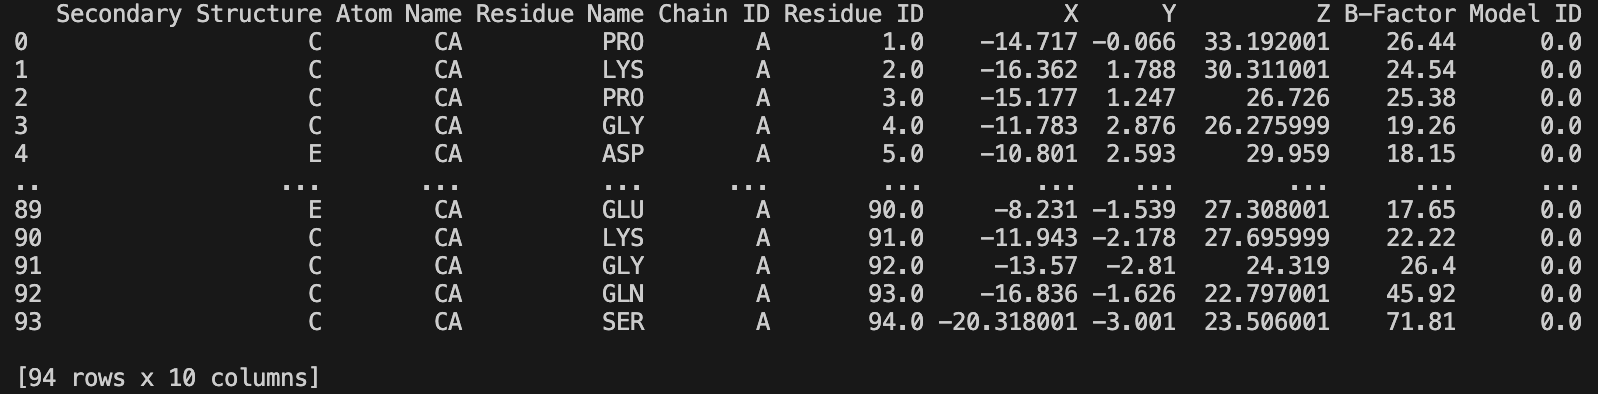
\includegraphics[width=0.8\textwidth]{/Users/enrico/PROTEINS/tesi/immagini_tesi_ingelse/Screenshot 2024-12-11 at 12.00.12.png
    }
    \caption{Dataset of 3LNX.}
\end{figure}
We would expect that the allosteric sites are connected with the binding pocket, the region of the protein which is involved in the binding of the ligand.\\
So perturbing allosteric sites, that are in alpha-$\alpha$ we will observe a response around ligand site.\\ 
The movement that we expect in that region is a closing of the "two hands" of the protein, between beta-$\beta$ and alpha-$\alpha$.\\
So the complete dynamics expected is the following:\\
We have a signal in the allosteric sign, thus the protein, for example, open its hands, so the ligand can bind to the binding pocket.\\
Now the carboxylate binding loop bloch another protein that is coming and after that we expected another signal from the allosteric site that close the hands of the protein.\\



\newpage
\section{Connection Radius}\label{connection_radius}
\noindent A critical aspect of analyzing 3LNX’s structural data is the choice of the connection radius when constructing the Kirchhoff matrix, so the question is:\\
For composing the graph how long shuld i consider the interaction radius between the residues?\\
Obviosly if i choose a too short connection radius, i will lose the long-range interactions between the residues, if i choose a too long connection radius, i will lose the local interactions between the residues.\\
So i would like to select an appropriate connection radius, one captures both local and long-range interactions between residues, ensuring that the resulting network accurately reflects the protein’s mechanical and dynamic properties.
\begin{figure}[h!]
    \centering
    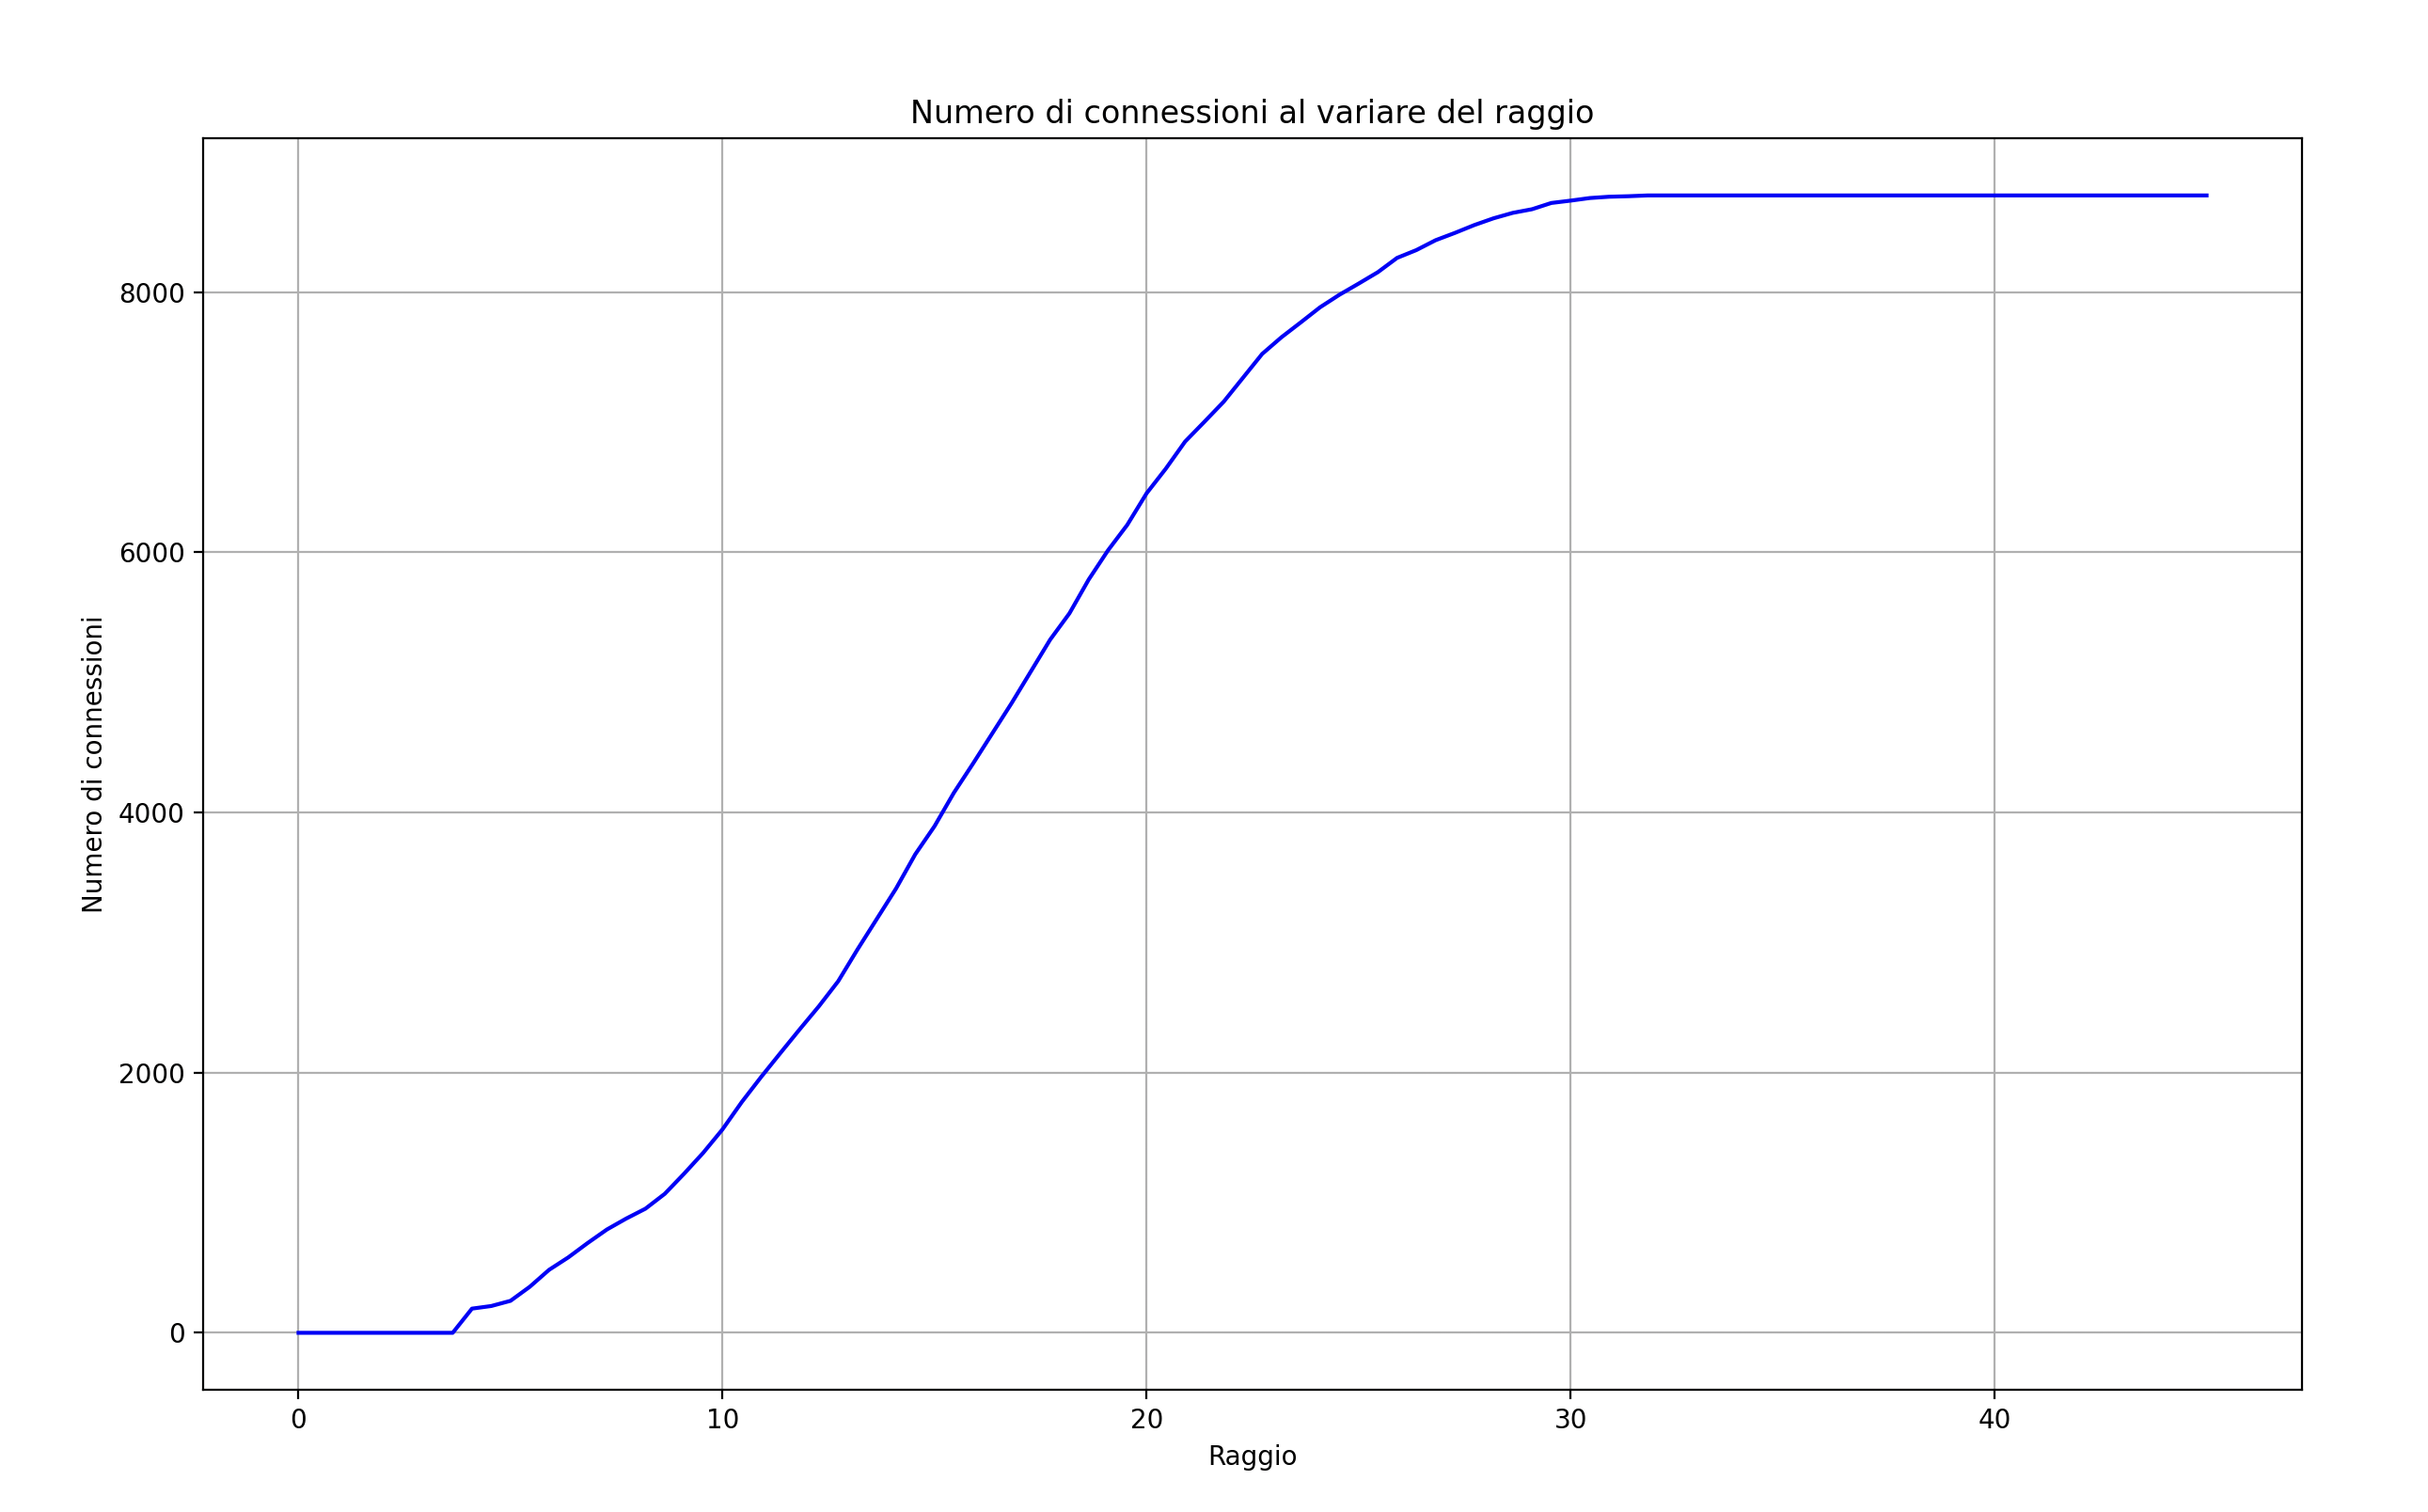
\includegraphics[width=0.8\textwidth]{/Users/enrico/PROTEINS/tesi/immagini_tesi_ingelse/Screenshot 2024-12-08 at 11.54.32.png}
    \caption{Number of links in function of the connection radius.}
\end{figure}

It is common in literature to take a value for the connection radius $\tilde{x} \approx \frac{1}{2} x^*, \text{ dove } x^* \text{ è tale che } f''(x) \big|_{x = x^*}$ = 0.\\
In our case we took the value of 8.0 nm.\\
\begin{figure}[h!]
    \centering
    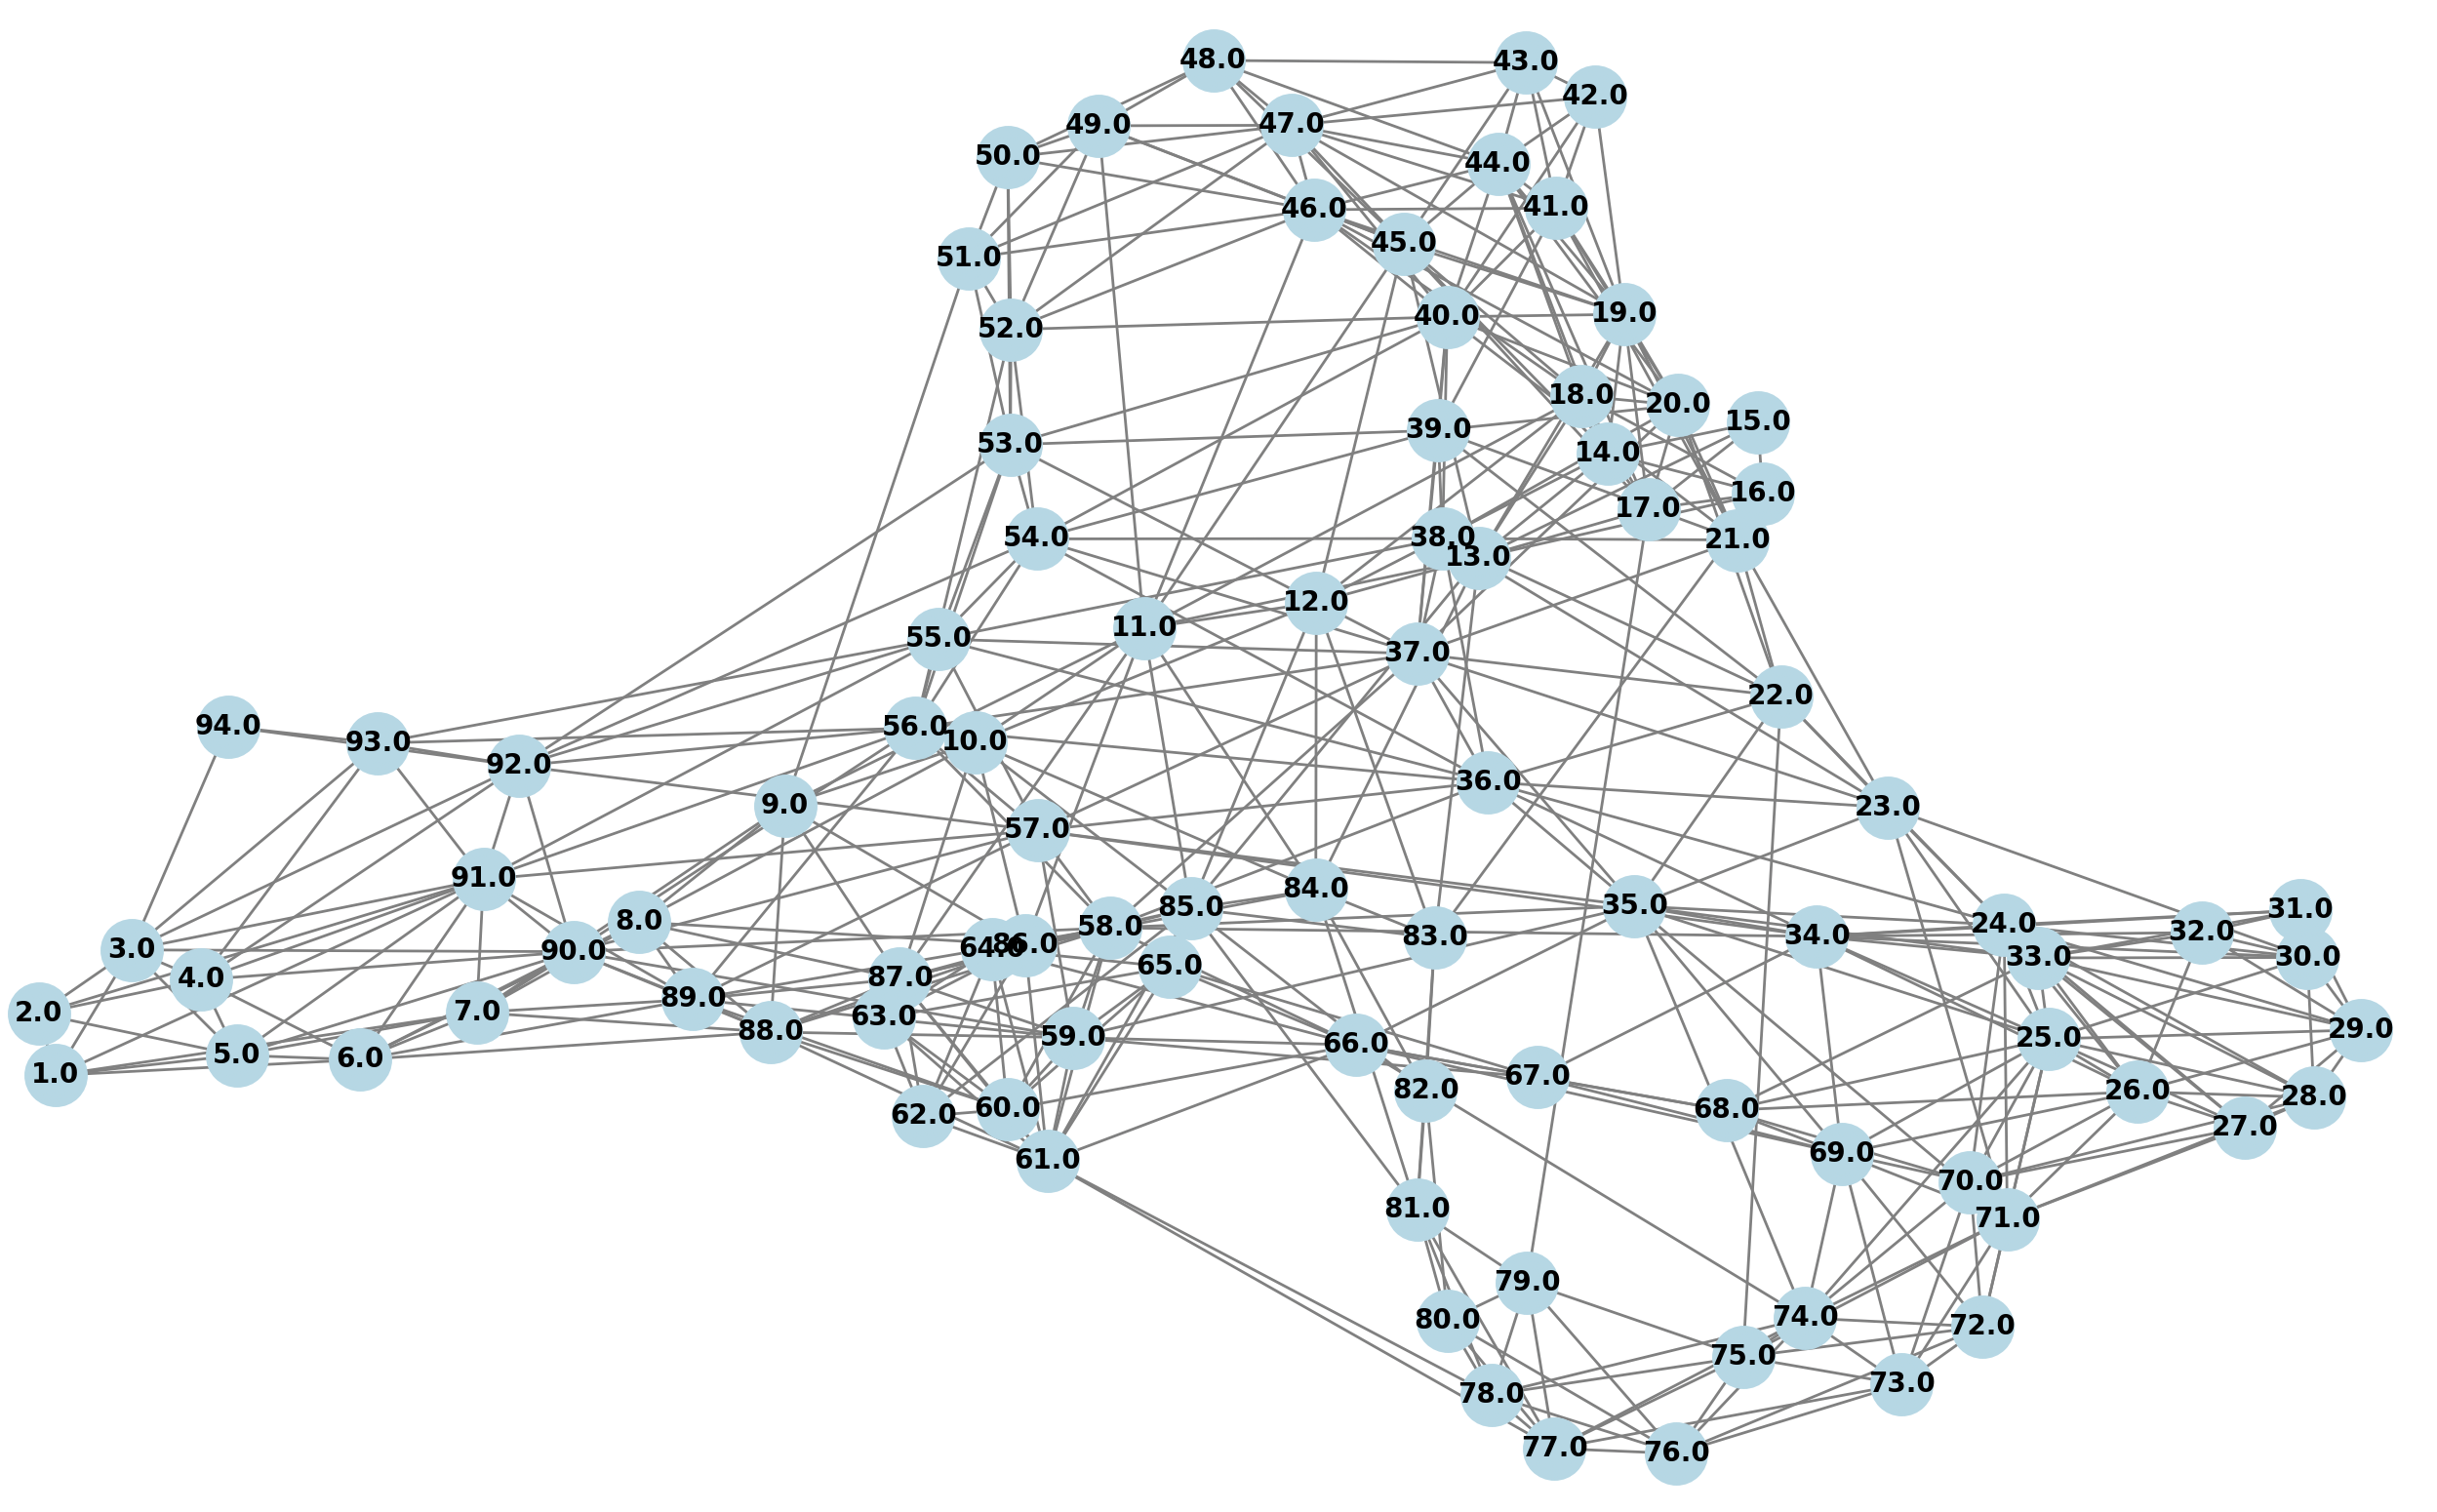
\includegraphics[width=0.8\textwidth]{/Users/enrico/PROTEINS/tesi/immagini_tesi_ingelse/Screenshot 2024-12-11 at 11.59.21.png}
    \label{fig:grafo_connessione}
    \caption{Bidirectional Graph obtained with radius of 8.0 .}
\end{figure}
Using that connection radius we obtain the following graph \figref{grafo_connessione}.
\newpage

\section{Kirchhoff Matrix}\label{Kirchhoff_paragraph}
\noindent 
By applying the Kirchhoff matrix \eqref{Kirchhoff} formulation to the protein structure, we derive the matrix K, which captures the connectivity between residues and provides insights into the protein’s dynamic properties.\\
The Kirchhoff matrix is a simplification that models the protein as a network of interactions, where the weights of the links represent the strength of the coupling between residues. However, this approximation assumes that the protein’s interactions can be described as a network of pairwise connections, ignoring more complex interactions such as solvation effects or multi-body interactions, which may also play a role in determining the protein’s overall behavior.\\
As we just said this matrix captures the connectivity between residues and provides insights into the protein's structural dynamics. \\
Now we can choose the weights of the links between the residues and in our case we choose to put the value of the link between two native pair (near neighbor), equal to 20, otherwise the link is equal to 1.\\
This is because typically the near neighbors are connected by strong covalent bonds (300–400 kJ/mol), or stabilized by dense non-covalent interactions (van der Waals forces, hydrogen bonds). 
These are typically 20 times grater than the intensity of connection between distant pairs of residues.\\
So, formally, i can write:
Let \( G = (V, E) \) be a graph where \( V \) is the set of vertices and \( E \) is the set of edges. Define the weight of the link between two vertices \( i \) and \( j \) as \( w(i, j) \).
We assign weights as follows:
\[
w(i, j) =
\begin{cases}
20, & \text{if } i \text{ and } j \text{ are near neighbors}, \\
1, & \text{otherwise}.
\end{cases}
\]

\begin{figure}[h!]
    \centering
    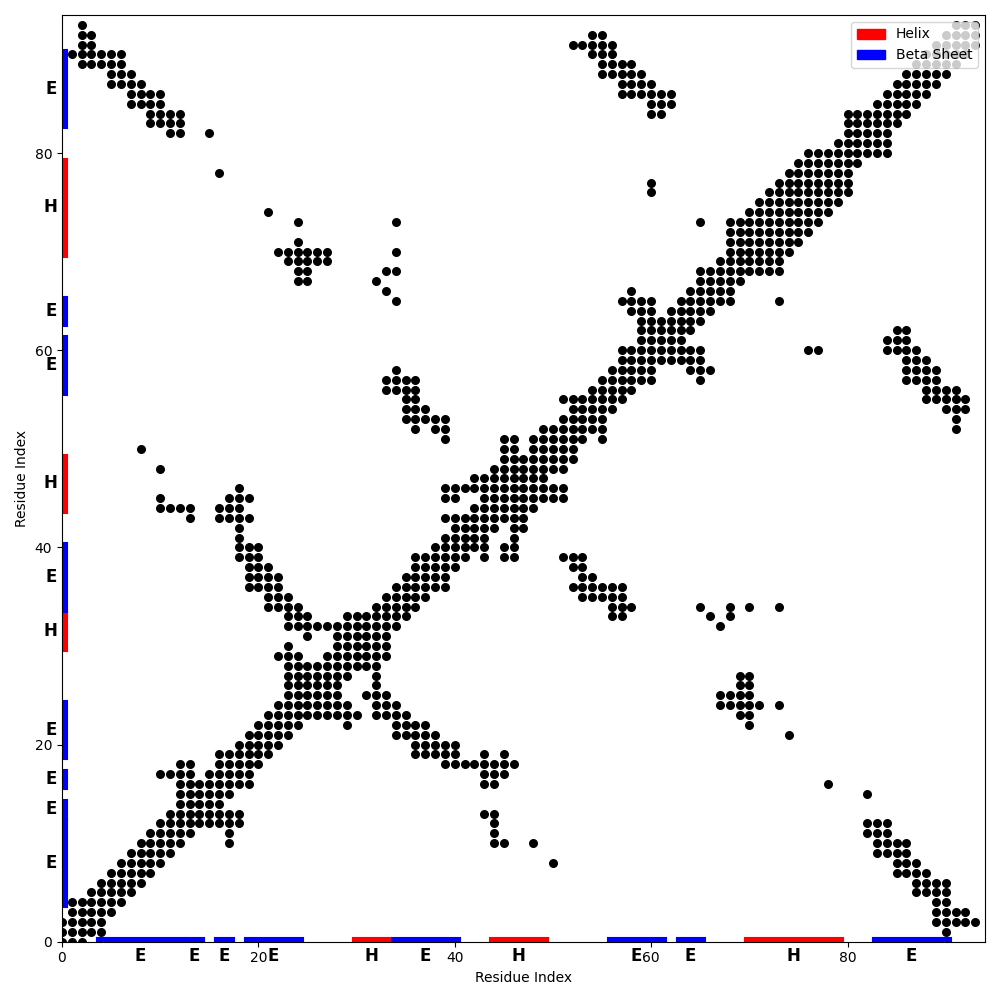
\includegraphics[width=0.8\textwidth]{/Users/enrico/PROTEINS/tesi/immagini_tesi_ingelse/Matrice di Kirchhoff della Proteina.png}\label{fig:kirchoff}
    \caption{Kirchoff Matrix.}
\end{figure}
And this is the representation of the Kirchhoff matrix of the protein structure \ref{kirchoff}.\\
\\\\\\\\\\\\\\
We notice first that as expected the Kirchhoff matrix is symmetric and that the diagonal elements are all negative. \\
This is consistent with the physical interpretation of the matrix, where the diagonal elements represent the sum of the coupling strengths between a residue and all other residues in the protein. The negative sign indicates that the interactions are stabilizing, as expected in a protein structure. The off-diagonal elements represent the coupling between pairs of residues, reflecting the network of interactions that stabilize the protein's structure.\\
It is important to notice also that most of the links are between near residues, but we have also some cluster of links between distant residues. This is important because it means that the protein is not a simple chain of residues but it is a complex network of interactions.
\newpage
\section{Covariance Matrix}
\noindent The two figures illustrate the covariance matrices obtained from the protein structure, one only plotting the positive covariance and the other only plotting the negative covariance.\\
The correlation matrix as we said before is defined as:
\[
C_{ij}(t) = \sum_{k=1}^N \frac{k_B T}{\lambda_k} u_{ik} u_{jk} e^{-\lambda_k t}.
\]
and so a time 0:\\
\[
C_{ij}(t) = \sum_{k=1}^N \frac{k_B T}{\lambda_k} u_{ik} u_{jk}.
\]
In the following figures we plot also the secondary structure (Helices: red; Beta Sheets: blue) and the kirchoff matrix.\\
\begin{figure}[h!]
    \centering
    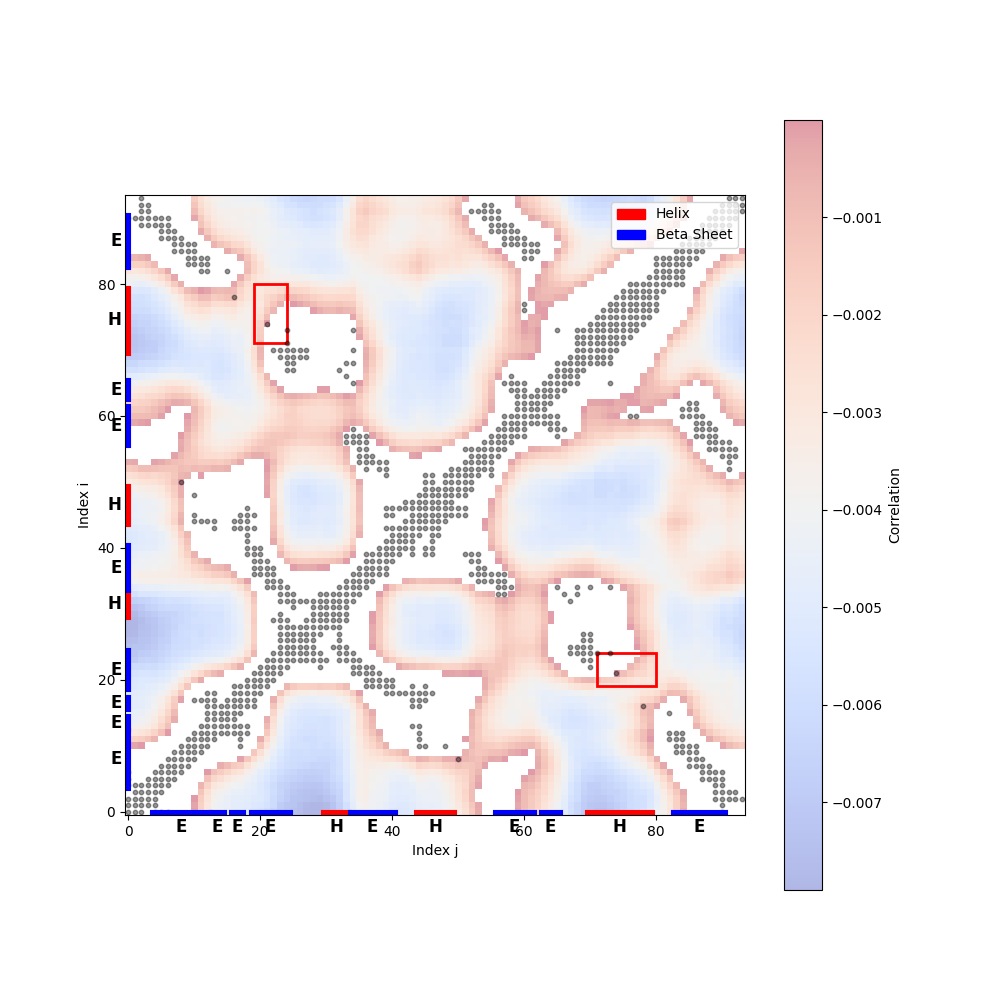
\includegraphics[width=0.8\textwidth]{/Users/enrico/PROTEINS/tesi/immagini_tesi_ingelse/Correlation_MatrixNan_False.png}
    \caption{Negative covariance between residues at time 0.}
    \label{fig:correlation_negative_figo}
\end{figure}

\begin{figure}[h!]
    \centering
    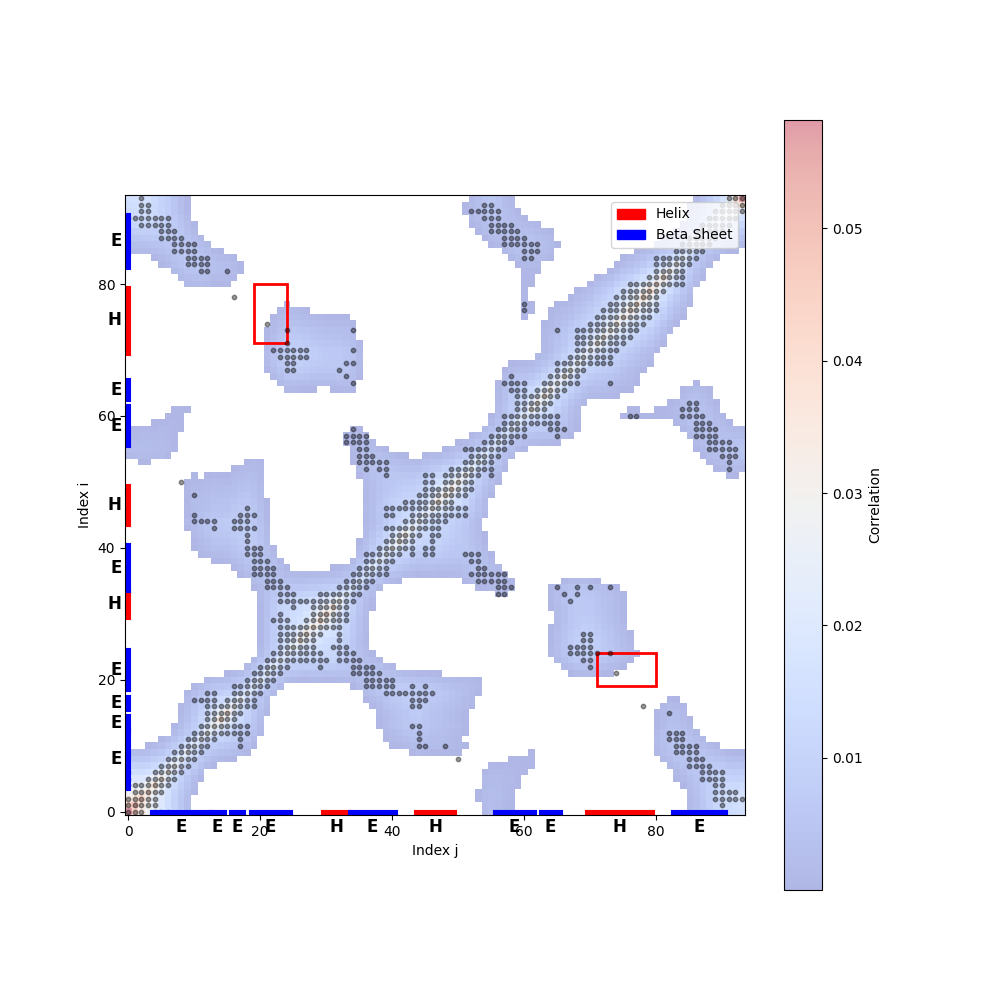
\includegraphics[width=0.8\textwidth]{/Users/enrico/PROTEINS/tesi/immagini_tesi_ingelse/Correlation_MatrixNan_True.png}
    \caption{Positive covariance between residues at time 0.}
    \label{fig:correlation_positive_figo}
\end{figure}
In these images we notice that we have positive correlation where we have residues and negative correlation where we don't have residues.
More distant is a region from the residues more negative will be the correlation.\\
We can see also a cluster of the most postive corerlation along the diagonal.\\
So the Kirchhoff matrix directly influences the correlation matrices by encoding the connectivity between residues. 

\newpage
\section{Beta Factors}
\noindent The plot above compares the experimental \( B \)-factors (blue curve), as we said in \eqref{beta} $B_i = 8\pi^2 C_{ii}$, with the predicted \( B \)-factors (red curve) along the residue index. \\
The \( B \)-factors represents the atomic displacement so they are a critical measure of the dynamic behavior of the protein structure. \\
They are also useful for testing the quality of the model.\\
\begin{figure}[h!]
    \centering
    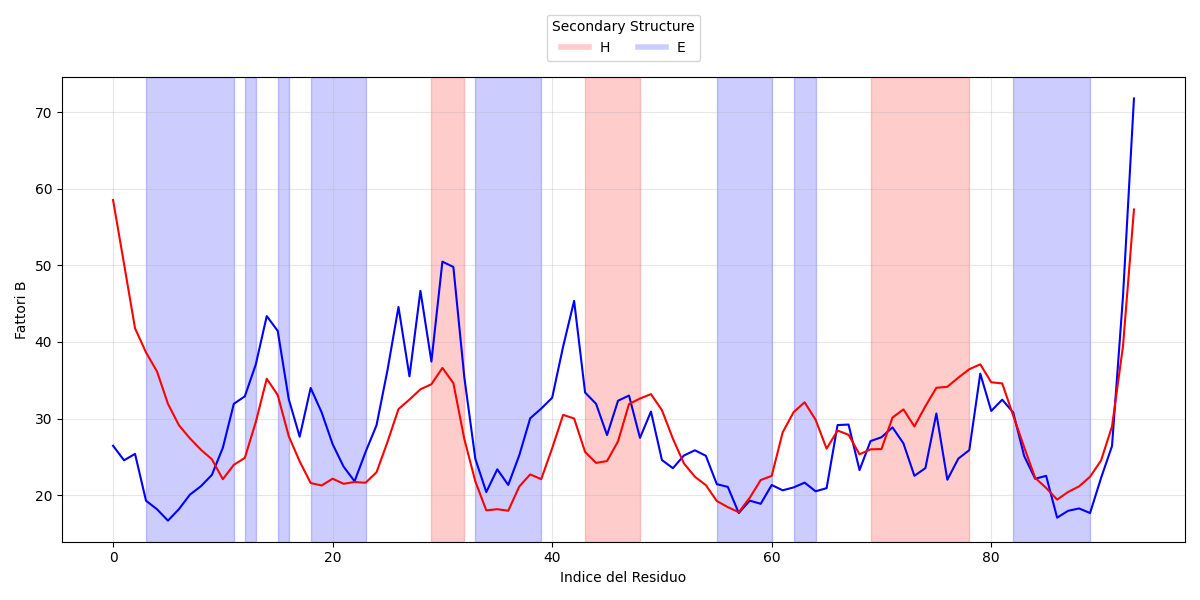
\includegraphics[width=0.8\textwidth]{/Users/enrico/PROTEINS/images/3LNX/beta_factors/Confronto_con_Struttura_Secondaria.png
    }
    \caption{Beta factors.}
\end{figure}
We see that the predicted \( B \)-factors generally follow the experimental trend, demonstrating the effectiveness of the model in capturing the dynamics of the protein.\\
Discrepancies between the predicted and experimental curves are visible in certain regions; these deviations may be due to limitations in the Kirchhoff matrix approximation or oversimplified assumptions in the modeling process.\\
Using formula of section \ref{sec:Evaluation}, we can evaluate the model performance by calculating the Root Mean Squared Error (RMSE) and Mean Absolute Error (MAE) between the predicted and experimental \( B \)-factors so we can have a quantitative measure of the model accuracy in capturing the protein's dynamic behavior.\\
\begin{table}[h!]
    \centering
    \begin{tabular}{|c|c|}
    \hline
    \textbf{Metric} & \textbf{Value} \\ \hline
    RMSE & 8.5200 \\ \hline
    MAE  & 6.4146 \\ \hline
    \end{tabular}
    \caption{Model Performance Metrics}
    \label{tab:model_metrics}
\end{table}
It is clear that we can improve the model and it is possible to obtain more accurate predictions.\\
Now let's valuate if the model can catch the allosteric dynamics of the protein.\\
\newpage
\section{Causal indicators in time}
\noindent Now we can plot the causal indicators in time.
\subsection{Correlation in time}
\noindent Let's start with the correlation in time, as we said before the correlation is defined as:
\[
C_{ij}(t) = \sum_{k=1}^N \frac{k_B T}{\lambda_k} u_{ik} u_{jk} e^{-\lambda_k t}.
\]
\begin{figure}[h!]
    \centering
    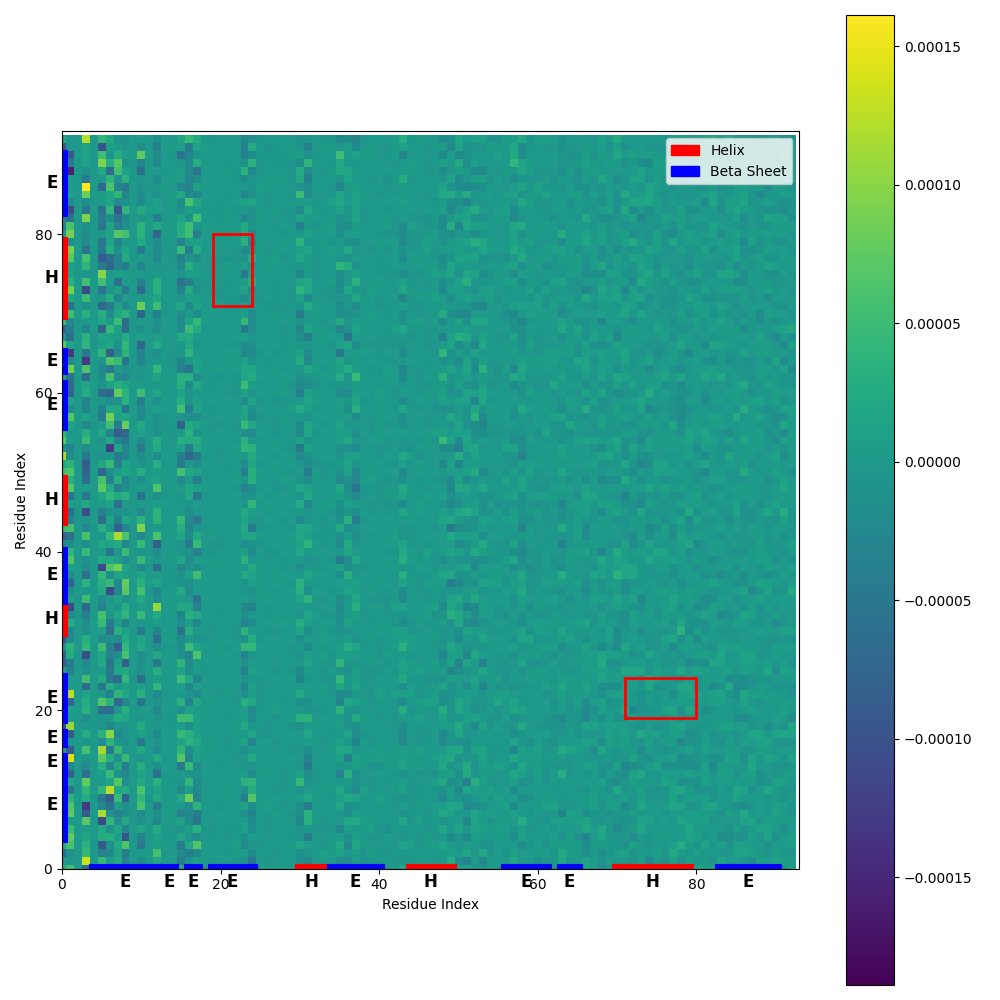
\includegraphics[width=0.8\textwidth]{/Users/enrico/PROTEINS/images/3LNX/Multiple_time_correlation/correlation.png}    
    \caption{Correlations in time.}
\end{figure}
This behavior is coherent with what expected, the correlation decay over time, indicating a loss of direct dynamic influence as time progresses.\\
Moreover correlation values vary significantly between residue pairs, reflecting differences in their initial dynamic coupling.\\
Finally residue pairs closer in space tend to show higher initial correlations compared to more distant pairs.

\subsection{Response in time}
\noindent The response in time is defined as we said before as:
\[
R_{\beta\gamma}(t) = \frac{\sum_{k=1}^N \frac{1}{\lambda_k} u_{\beta k} u_{\gamma k} e^{-\lambda_k t}}{\sum_{k=1}^N \frac{1}{\lambda_k} u_{\beta k} u_{\gamma k}}.
\]

\begin{figure}[h!]
    \centering
    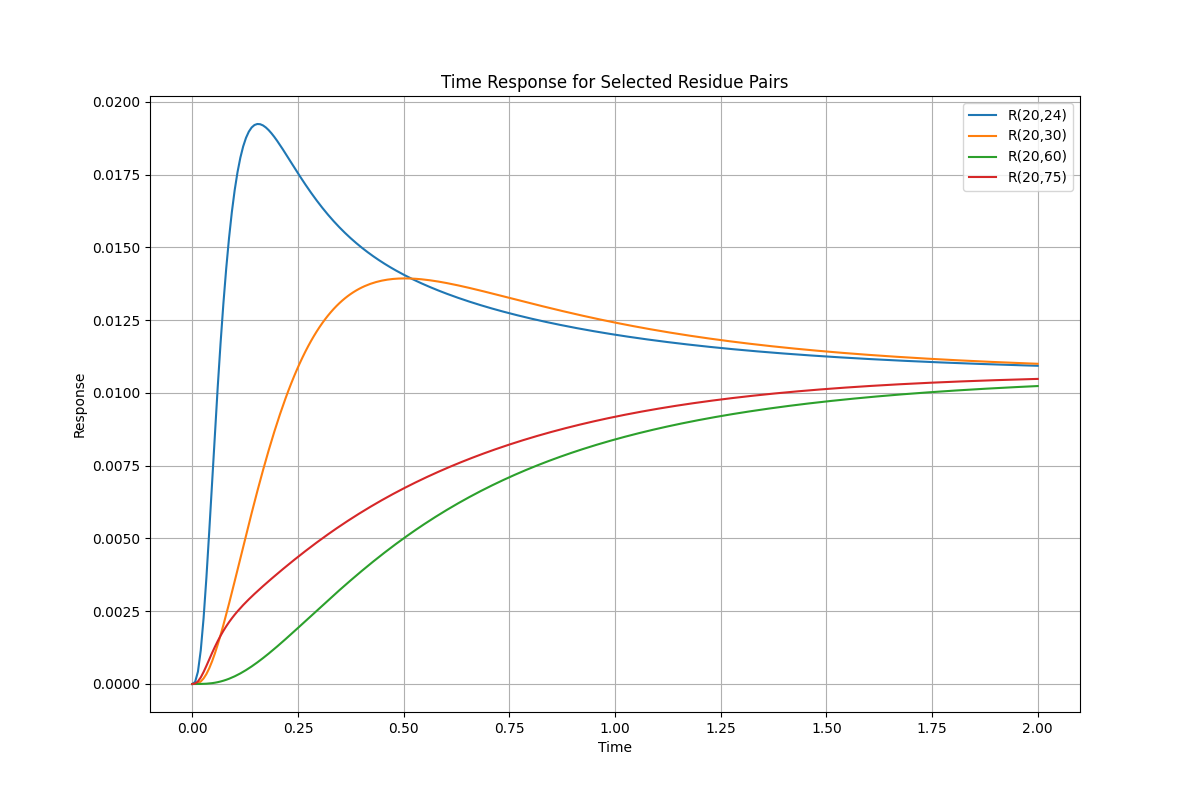
\includegraphics[width=0.8\textwidth]{/Users/enrico/PROTEINS/images/3LNX/Multiple_time_resposne/risposte.png}    
    \caption{Responses in time.}
\end{figure}

This behavior is coherent with what expected, the correlation decay over time, indicating a loss of direct dynamic influence as time progresses.\\
Also we notice that when correlation can be positive or negative, the response is always positive, starting from 0 and reaching the value of 1/N\\
The responses exhibit a sharp rise initially, which is then followed by a gradual decay.
residue pairs closer to the source of perturbation (likely spatially proximal) show a more pronounced and faster response.
A peak is observed at an intermediate time point for most residue pairs, indicating a time of maximum information transfer.
        

\subsection{Transfer entropy in time}
\noindent In this image we see that a peak is observed at an intermediate time point for most residue pairs, indicating a time of maximum information transfer, in addition the magnitude of transfer entropy varies, reflecting differences in the strength of directional coupling between pairs and residue pairs with high initial connectivity (likely closer in the protein structure) exhibit stronger peaks compared to those that are more distant.\\
\begin{figure}[h!]
    \centering
    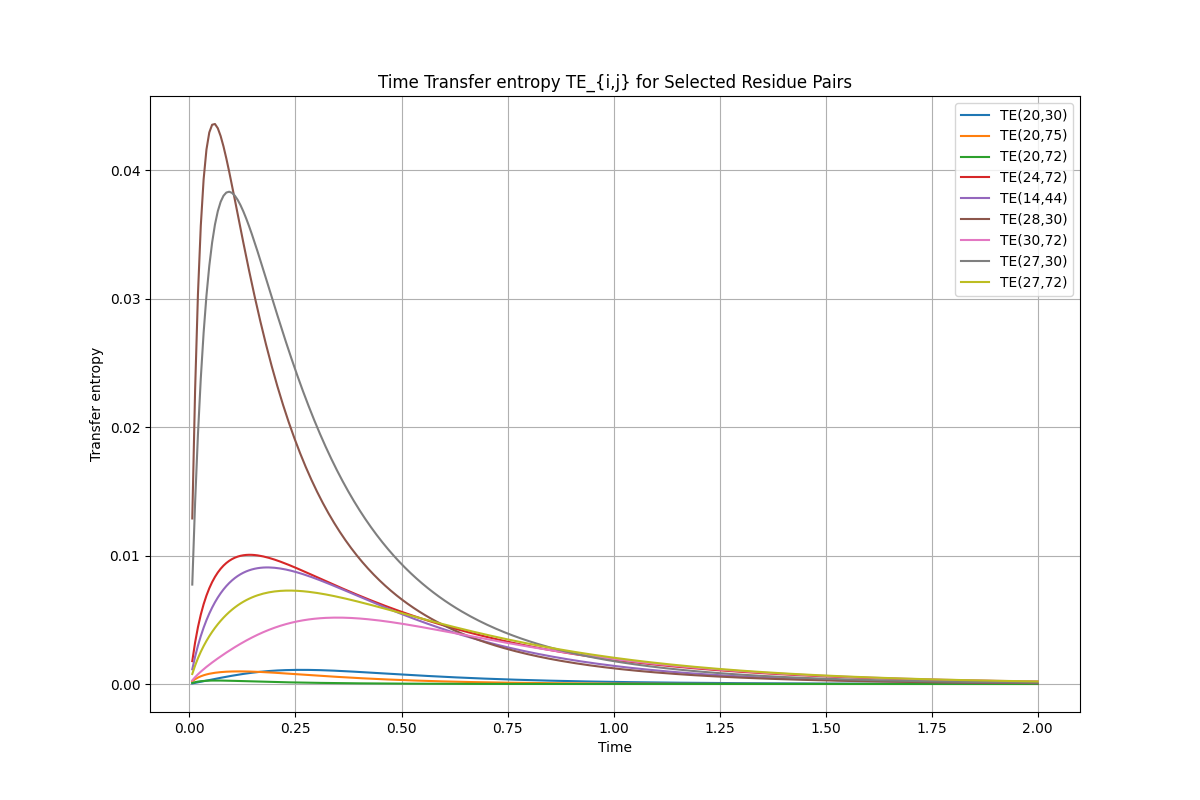
\includegraphics[width=0.8\textwidth]{/Users/enrico/PROTEINS/images/3LNX/Multiple_time_correlation/entropy.png}    
    \caption{Transfer entropy  in time.}
\end{figure}


\newpage

\section{Causal indicators between residues}
\subsection{Introduction}
\noindent In this section we will focus on the causal indicators between residues.\\ 
This is the main section of our work in which we will try to understand the allosteric mechanism of the protein and understand for real if the model explain in a good way the protein dynamics.\\
As we said before if the graph of the proteins were random we will expected random interaction.\\ 
For seeing if our model is in according with the real world results if we perturb the allosteric sites, situated in according with paper \cite{ref15} in all the alpha-$\alpha$ and alpha-$\gamma$ helices, we will expected that the signal will propagate along the protein structure for reaching the active sites, around beta-$\beta$ and Alpha-$\alpha$.\\

\subsection{characteristic time determination}
\noindent To analyze our system, it is essential to focus on timescales around the characteristic time \(\tau\). \\
In fact if the time \(t\), in which we analyze the system, is too short so we don't see in a right way the propagation, in other hand if the time is too long we don't see the relaxation of the system.\\
So to determine the characteristic time \(\tau\) of the system, we have to analyze the autocorrelation function \(C_{i,i}(t)\) between all residues for all relevant times \(t\). \\
The idea is that the mean of typical decay time is the characteristic time \(\tau\) of my system.\\
Mathematically for each index \(i\)  will take the autocorrelations \(C_{i,i}(t)\) when they are equal to \(e^{-1}\) of their initial values. These times are the \(t_i\) for every residues.\\
Now i have an histogram of times and taking the mean of this vlaues i will obtain my characteristic time \(\tau\).\\
\begin{figure}[h!]
    \centering
    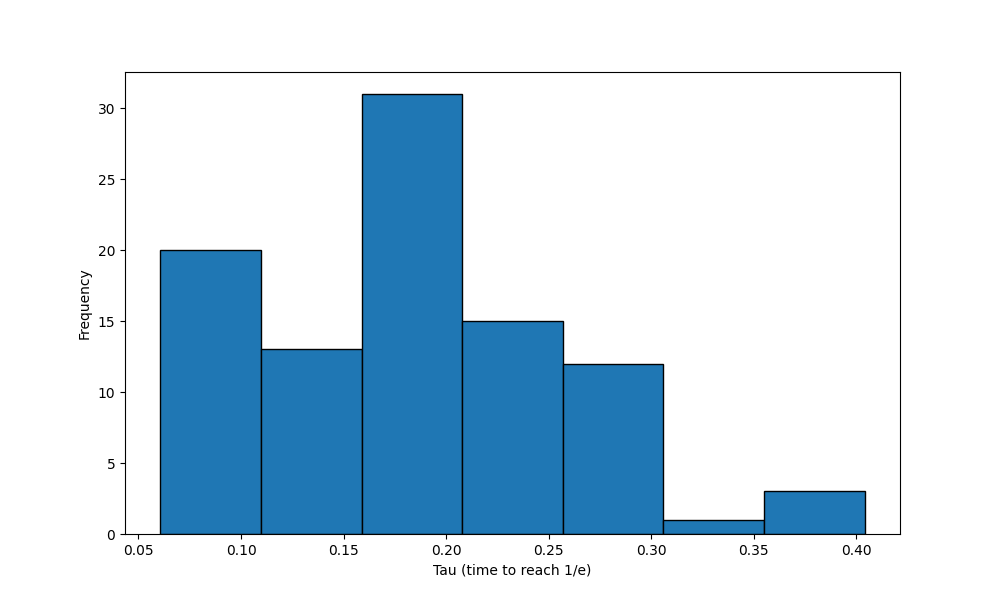
\includegraphics[width=0.8\textwidth]{/Users/enrico/PROTEINS/images/3LNX/2_temperature_cutoff/Stima_tau/tau_histogram.png}
    \caption{Hisotgram of \(t_i\).}
\end{figure} 

\begin{figure}[h!]
    \centering
    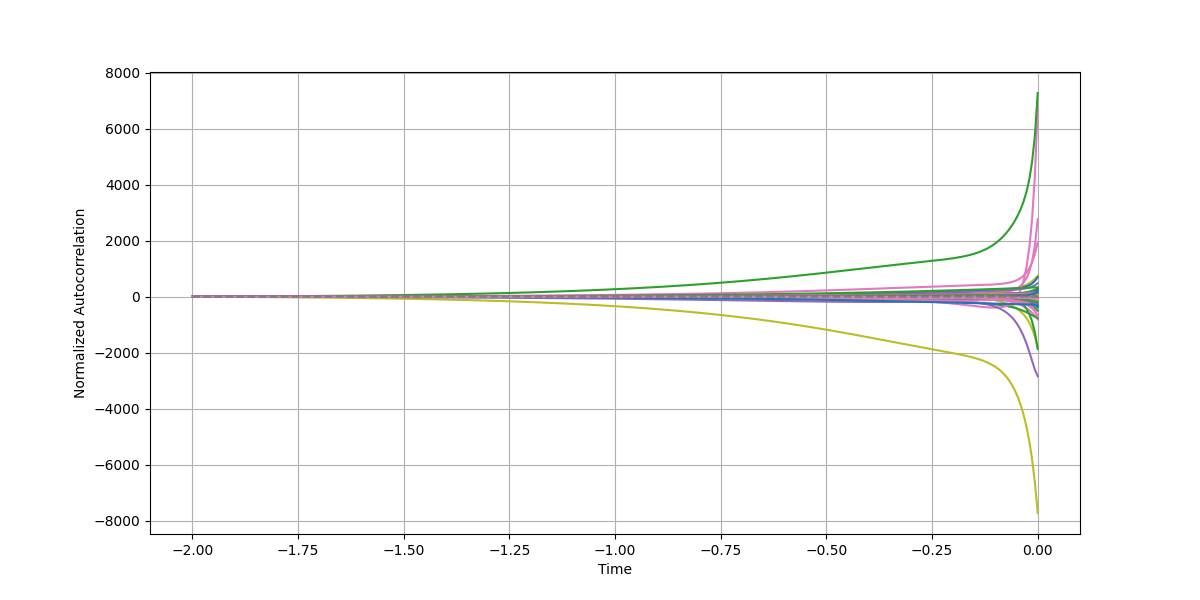
\includegraphics[width=0.8\textwidth]{/Users/enrico/PROTEINS/images/3LNX/Stima_tau/autocorrelation_fits.png}
    \caption{Fit of tau.}
\end{figure}
We estimated a time \(\tau\) of 0.1842 ns.\\



All the following analysis will be done around the characteristic time \(\tau\), specifically at [\(\tau\)-0.5*\(\tau\),\(\tau\),\(\tau\)+0.5*\(\tau\)].
\newpage
\subsection{Correlation between residues}
\noindent We plotted here the correlation between one specific residues at time \(\tau\) and all the residues.\\
\begin{figure}[h!]
    \centering
    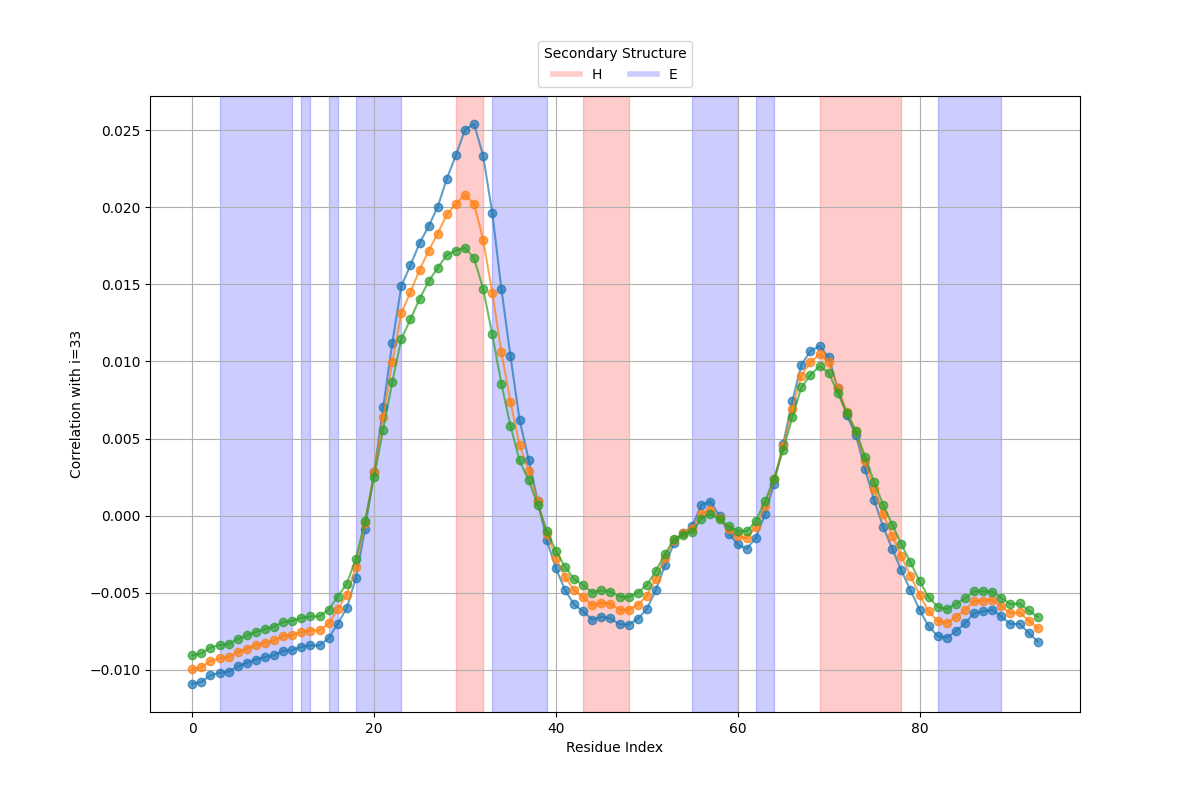
\includegraphics[width=0.8\textwidth]{/Users/enrico/PROTEINS/images/3LNX/Time_indicators/Residual Correlation C_ij for i=33 as a function of j at time index 0.png}
    \caption{Correlation of 34-th residue}
    \label{fig:Correlation of 34-th residue}
\end{figure}
\begin{figure}[h!]
    \centering
    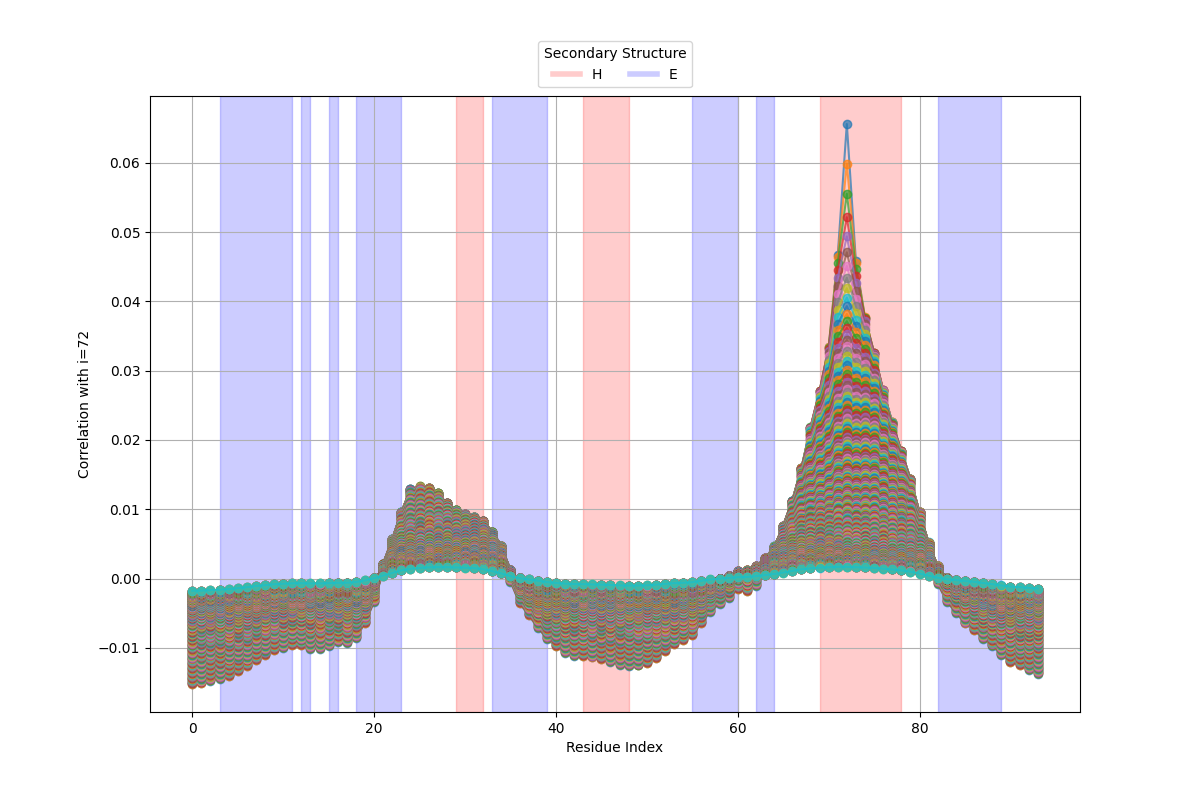
\includegraphics[width=0.8\textwidth]{/Users/enrico/PROTEINS/images/3LNX/Time_indicators/Residual Correlation C_ij for i=72 as a function of j at time index 0.png}
    \caption{Correlation of 73-th residue}
    \label{fig:Correlation of 73-th residue}
\end{figure}


\subsubsection{Results and Discussion}
\noindent Considering image \figref{Correlation of 34-th residue} we see that the correlation with i=34 has a clear and well-defined local correlation peak emerges around residue i=34.\\
As we expected, and we are happy about it, we observe a high correlation in modules in the region of the binding pocket, between alpha-$\alpha$ and beta-$\beta$, and in the other allosteric site in the alpha-$\gamma$ helix, that represents a comunication between allosteric regions.\\
There are also moderate responses observed in the alpha-$\beta$-helix region. \\
\\\\\\\\\
\begin{tikzpicture}[node distance=2cm]

    % Nodes for perturbation and regions
    \node (alphaalpha) [draw, rectangle, text centered, minimum height=1cm, minimum width=2cm] {Perturbazione alpha-$\alpha$ helix};
    
    % Nodes for regions below alpha-alpha, aligned horizontally with extra spacing
    \node (binding) [below of=alphaalpha, draw, rectangle, text centered, minimum height=1cm, minimum width=2.5cm, xshift=-6cm, yshift=-1cm] {Binding Pocket}; 
    \node (alphaGamma) [below of=alphaalpha, draw, rectangle, text centered, minimum height=1cm, minimum width=2.5cm, xshift=-3cm, yshift=-1cm] {alpha-$\gamma$};
    
    % Optional: add head and tail nodes if needed
    \node (head) [below of=alphaalpha, draw, rectangle, text centered, minimum height=1cm, minimum width=2.5cm, xshift=3cm, yshift=-1cm] {Head};
    \node (tail) [below of=alphaalpha, draw, rectangle, text centered, minimum height=1cm, minimum width=2.5cm, xshift=6cm, yshift=-1cm] {Tail};

    % Draw arrows from alpha-alpha to each region
    \draw[->] (alphaalpha) -- (head);
    \draw[->] (alphaalpha) -- (tail);
    \draw[->] (alphaalpha) -- (binding);
    \draw[->] (alphaalpha) -- (alphaGamma);

\end{tikzpicture}


Now conisdering image \figref{Correlation of 73-th residue} we notice that there is a correlation peak for the correlation with i=73.\\
A dynamic relationship between the alpha-$\beta$-helix and the binding pocket is highlighted by the clear responses that take place in the binding pocket areas, such as the bet-$\beta$-strand and alpha$\alpha$-helix. 
So now we have the necessary relations for the causal relation between the allosteric site and the binding pocket.\\
Now let's indagate further.\\\\
\begin{tikzpicture}[node distance=2cm]

    % Nodes for perturbation and regions
    \node (alphaalpha) [draw, rectangle, text centered, minimum height=1cm, minimum width=2cm] {Perturbazione alpha-$\gamma$ helix};
    
    % Nodes for regions below alpha-alpha, aligned horizontally with extra spacing
    \node (binding) [below of=alphaalpha, draw, rectangle, text centered, minimum height=1cm, minimum width=2.5cm, xshift=-6cm, yshift=-1cm] {Binding Pocket}; 
    \node (alphaGamma) [below of=alphaalpha, draw, rectangle, text centered, minimum height=1cm, minimum width=2.5cm, xshift=-3cm, yshift=-1cm] {alpha-$\alpha$};
    
    % Optional: add head and tail nodes if needed
    \node (head) [below of=alphaalpha, draw, rectangle, text centered, minimum height=1cm, minimum width=2.5cm, xshift=3cm, yshift=-1cm] {Head};
    \node (tail) [below of=alphaalpha, draw, rectangle, text centered, minimum height=1cm, minimum width=2.5cm, xshift=6cm, yshift=-1cm] {Tail};

    % Draw arrows from alpha-alpha to each region
    \draw[->] (alphaalpha) -- (head);
    \draw[->] (alphaalpha) -- (tail);
    \draw[->] (alphaalpha) -- (binding);
    \draw[->] (alphaalpha) -- (alphaGamma);

\end{tikzpicture}







\subsection{Response between residues}
\begin{figure}[h!]
    \centering
    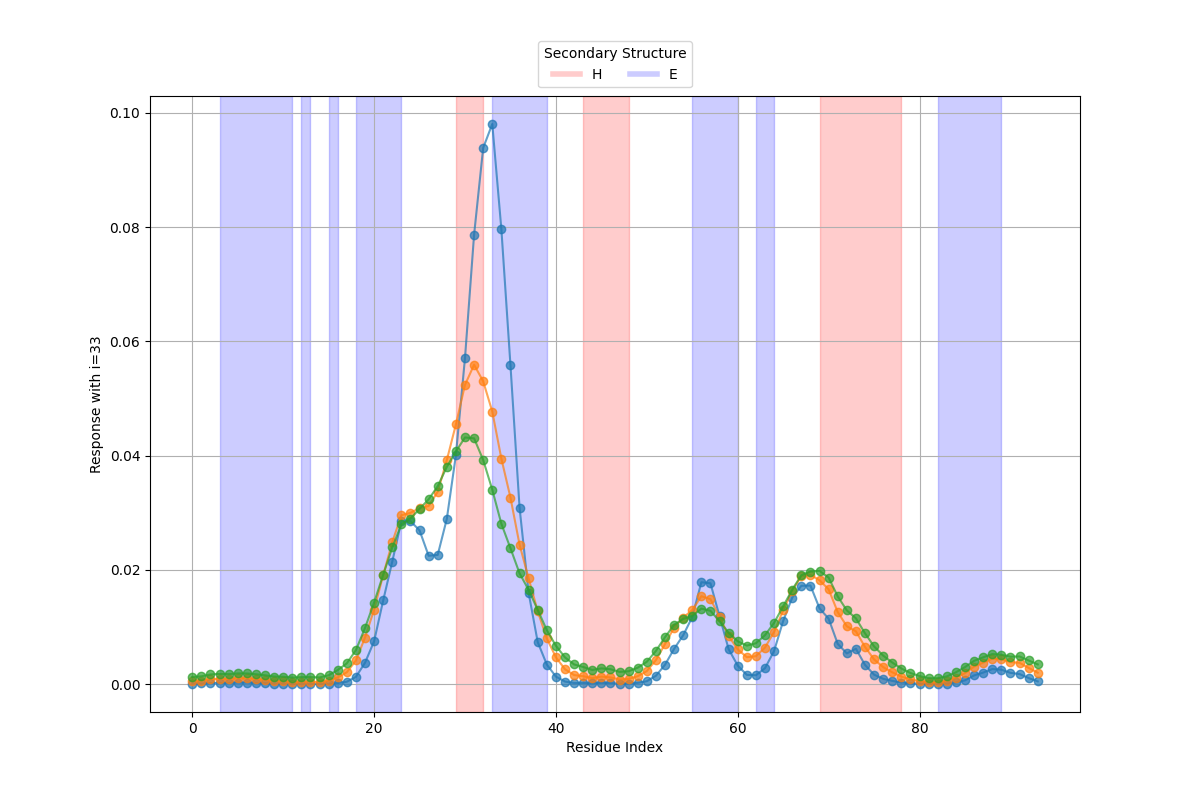
\includegraphics[width=0.8\textwidth]{/Users/enrico/PROTEINS/images/3LNX/Time_indicators/Time Response R_ij for i=33 as a function of j at time index 0.png}
    \caption{Response perturbating 34-th residue.}
    \label{fig:resp34}
\end{figure}



Pertubating the 34-th residue we see a clear response \figref{resp34} in the beta-$\beta$, in beta-$\delta$ and alpha-$\alpha$ helix, so we have a clear propagation of the signal from the allosteric site to the binding pocket.\\
This is good because it exludes the precedent hypotesis of the signals in the head and in the tail of the protein, where we had a high covariance.\\
Because we don't have a covariance signals in beta-$\delta$ we can't speak about causality. 
So excluding from the causal graph the non causal interaction we have this new representation:\\




\begin{tikzpicture}[node distance=2cm]

    % Nodes for perturbation and regions
    \node (alphaalpha) [draw, rectangle, text centered, minimum height=1cm, minimum width=2cm] {Perturbazione alpha-$\alpha$ helix};
    
    % Nodes for regions below alpha-alpha, aligned horizontally with extra spacing
    \node (binding) [below of=alphaalpha, draw, rectangle, text centered, minimum height=1cm, minimum width=2.5cm, xshift=-6cm, yshift=-1cm] {Binding Pocket}; 
    \node (alphaGamma) [below of=alphaalpha, draw, rectangle, text centered, minimum height=1cm, minimum width=2.5cm, xshift=6cm, yshift=-1cm] {alpha-$\gamma$};
    
    
    % Draw arrows from alpha-alpha to each region
    
    \draw[->] (alphaalpha) -- (binding);
    \draw[->] (alphaalpha) -- (alphaGamma);

\end{tikzpicture}


\\\\\\\\\\\\\\\\\\
\begin{figure}[h!]
    \centering
    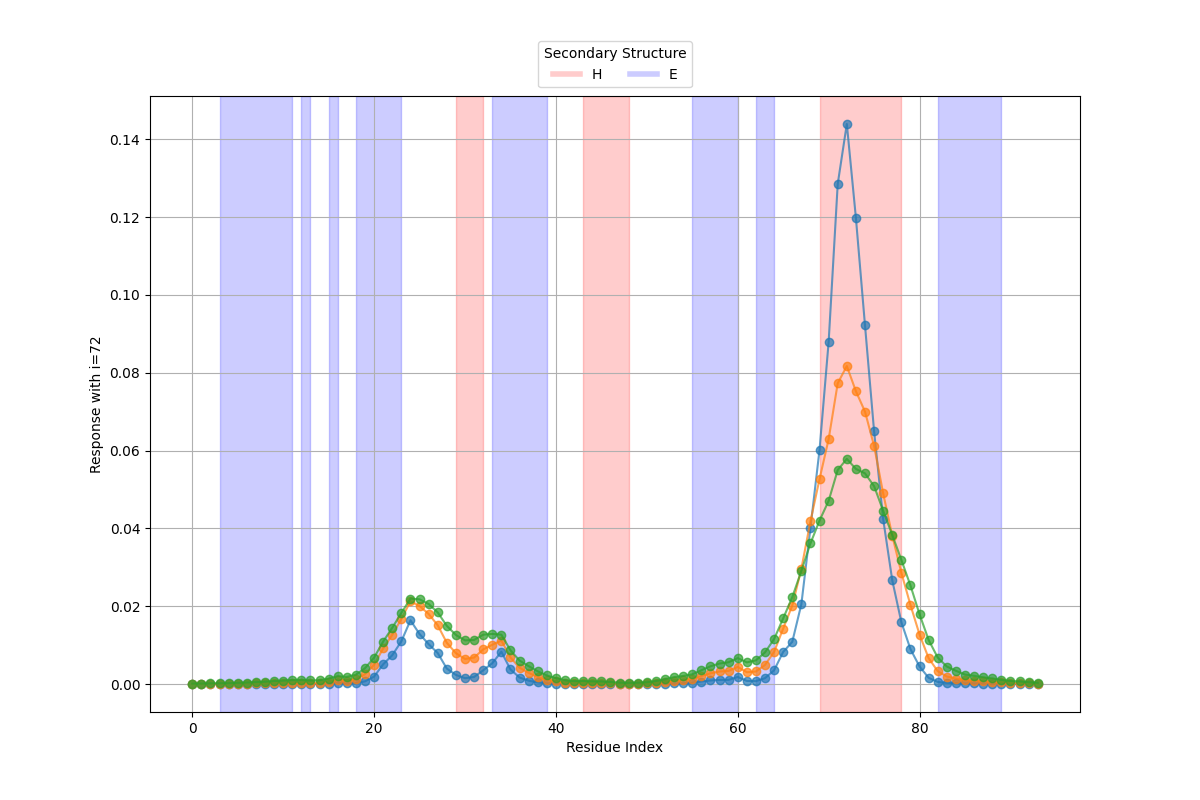
\includegraphics[width=0.8\textwidth]{/Users/enrico/PROTEINS/images/3LNX/Time_indicators/Time Response R_ij for i=72 as a function of j at time index 0.png}
    \caption{Response perturbating 73-th residue.}
    \label{fig:resp73}
\end{figure}\\\\\\\\\\

Now Pertubating the 73-th residue we see a clear response \figref{resp73} in the binding pocket, in the alpha-$\beta$ and a little bit in the beta-$\gamma$.
So now we have:
\begin{tikzpicture}[node distance=2cm]

    % Nodes for perturbation and regions
    \node (alphaalpha) [draw, rectangle, text centered, minimum height=1cm, minimum width=2cm] {Perturbazione alpha-$\gamma$ helix};
    
    % Nodes for regions below alpha-alpha, aligned horizontally with extra spacing
    \node (binding) [below of=alphaalpha, draw, rectangle, text centered, minimum height=1cm, minimum width=2.5cm, xshift=-6cm, yshift=-1cm] {Binding Pocket}; 
    \node (alphaGamma) [below of=alphaalpha, draw, rectangle, text centered, minimum height=1cm, minimum width=2.5cm, xshift=6cm, yshift=-1cm] {alpha-$\alpha$};
    
    
    % Draw arrows from alpha-alpha to each region
    
    \draw[->] (alphaalpha) -- (binding);
    \draw[->] (alphaalpha) -- (alphaGamma);

\end{tikzpicture}


\newpage
\subsection{Active Transfer entropies between residues}
\begin{figure}[h!]
    \centering
    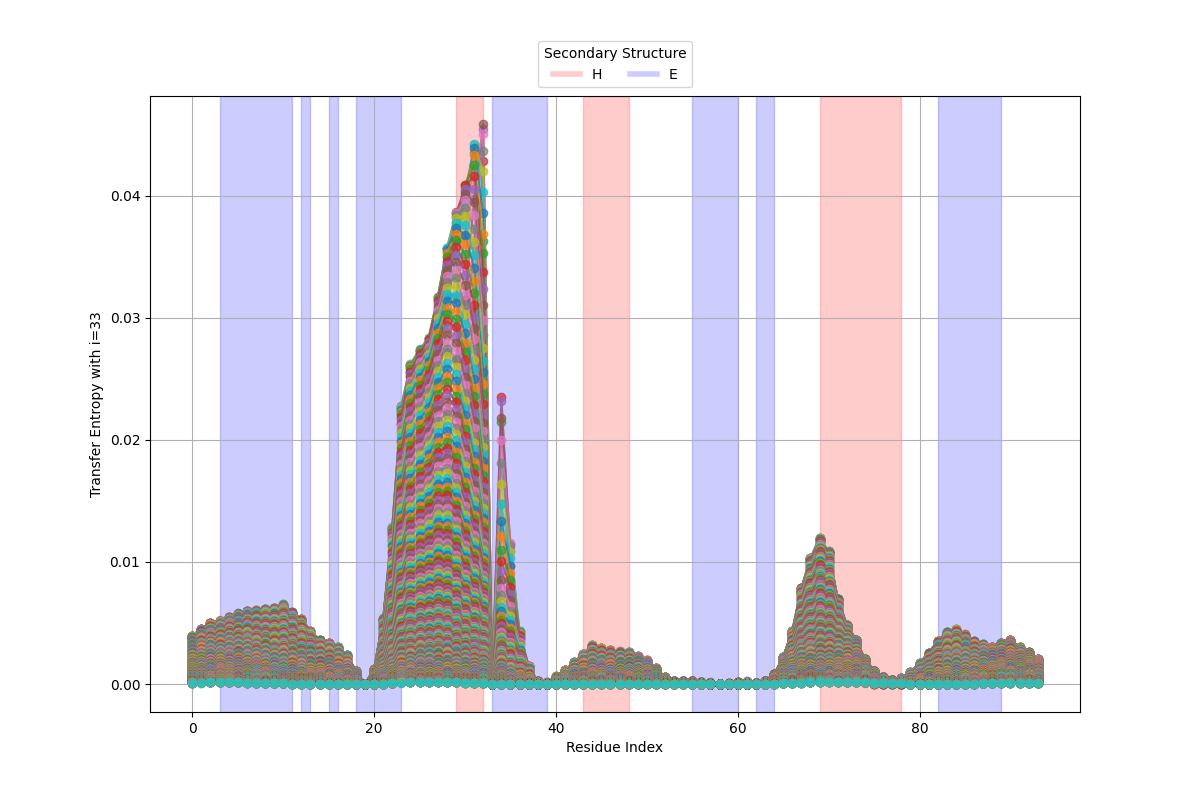
\includegraphics[width=0.8\textwidth]{/Users/enrico/PROTEINS/images/3LNX/Time_indicators/Transfer Entropy TE_ij for i=33 as a function of j at time index 0.png}
    \caption{Transfer Entropy j->34 (T_{34,j}).}
    \label{fig:TE34}
\end{figure}
We can see that the signal is propagated in the binding pocket and in the alpha-$\gamma$ helix.\\
It is a pattern vey similar to the response, suggesting a strong but not complete linear relation in the signal propagation.\\
So the graph of the causal relation remain the following:\\
\begin{tikzpicture}[node distance=2cm]

    % Nodes for perturbation and regions
    \node (alphaalpha) [draw, rectangle, text centered, minimum height=1cm, minimum width=2cm] {Perturbazione alpha-$\alpha$ helix};
    
    % Nodes for regions below alpha-alpha, aligned horizontally with extra spacing
    \node (binding) [below of=alphaalpha, draw, rectangle, text centered, minimum height=1cm, minimum width=2.5cm, xshift=-6cm, yshift=-1cm] {Binding Pocket}; 
    \node (alphaGamma) [below of=alphaalpha, draw, rectangle, text centered, minimum height=1cm, minimum width=2.5cm, xshift=6cm, yshift=-1cm] {alpha-$\gamma$};
    
    
    % Draw arrows from alpha-alpha to each region
    
    \draw[->] (alphaalpha) -- (binding);
    \draw[->] (alphaalpha) -- (alphaGamma);

\end{tikzpicture}




\begin{figure}[h!]
    \centering
    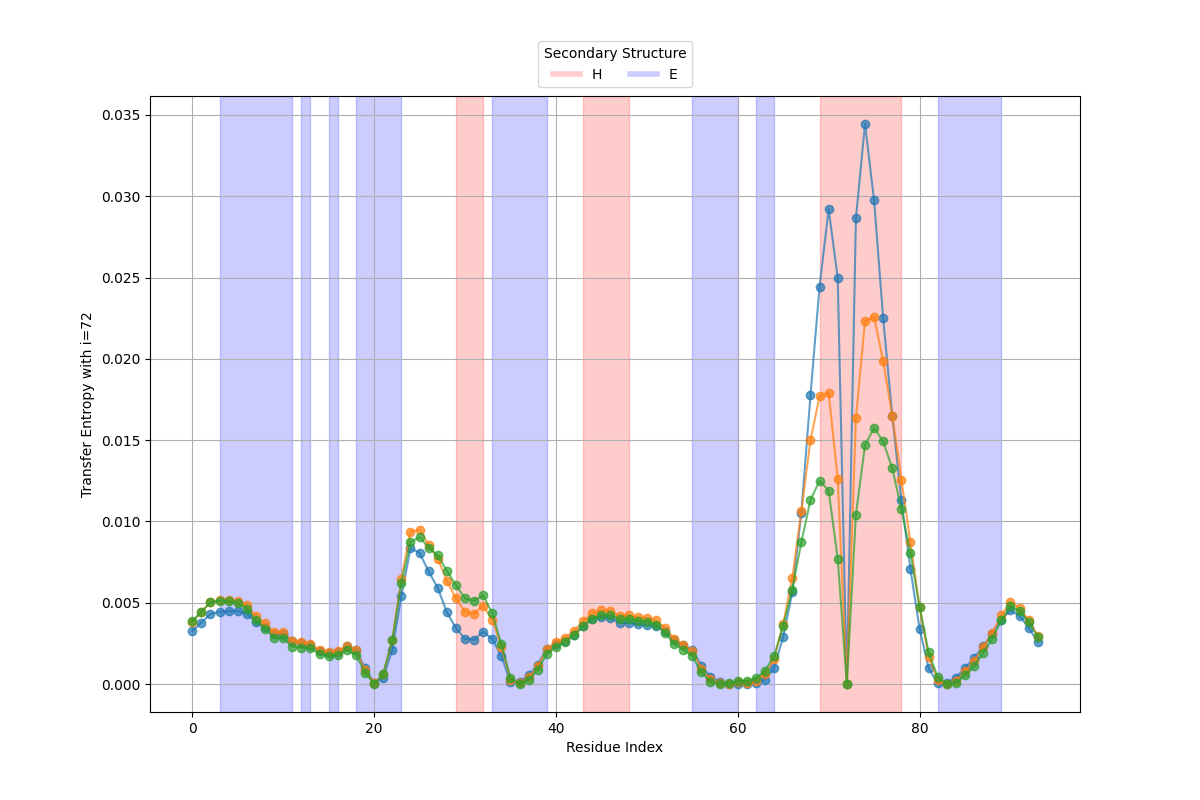
\includegraphics[width=0.8\textwidth]{/Users/enrico/PROTEINS/images/3LNX/Time_indicators/Transfer Entropy TE_ij for i=72 as a function of j at time index 0.png}
    \caption{Transfer Entropy j->73 (T_{73,j}).}
    \label{fig:TE73}
\end{figure}

The same argument of the previous case can be done for the 73-th residue.\\
\begin{tikzpicture}[node distance=2cm]

    % Nodes for perturbation and regions
    \node (alphaalpha) [draw, rectangle, text centered, minimum height=1cm, minimum width=2cm] {Perturbazione alpha-$\gamma$ helix};
    
    % Nodes for regions below alpha-alpha, aligned horizontally with extra spacing
    \node (binding) [below of=alphaalpha, draw, rectangle, text centered, minimum height=1cm, minimum width=2.5cm, xshift=-6cm, yshift=-1cm] {Binding Pocket}; 
    \node (alphaGamma) [below of=alphaalpha, draw, rectangle, text centered, minimum height=1cm, minimum width=2.5cm, xshift=6cm, yshift=-1cm] {alpha-$\alpha$};
    
    
    % Draw arrows from alpha-alpha to each region
    
    \draw[->] (alphaalpha) -- (binding);
    \draw[->] (alphaalpha) -- (alphaGamma);

\end{tikzpicture}
\newpage
\subsection{Passive Transfer entropies between residues }

\begin{figure}[h!]
    \centering
    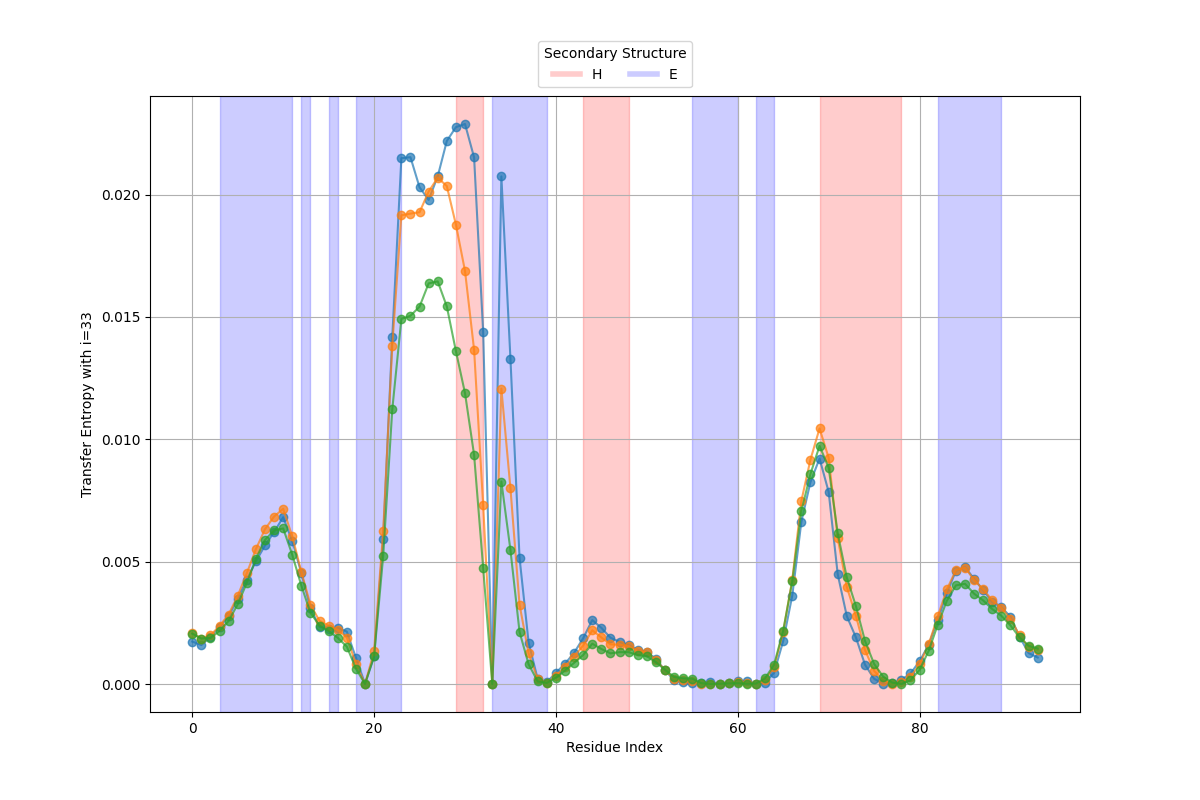
\includegraphics[width=0.8\textwidth]{/Users/enrico/PROTEINS/images/3LNX/Time_indicators/Transfer Entropy TE_ji for i=33 as a function of j at time index 0.png}
    \caption{Transfer Entropy 34->i (T_{i,34}).}
    \label{fig:TE34_pass}
\end{figure}

\begin{figure}[h!]
    \centering
    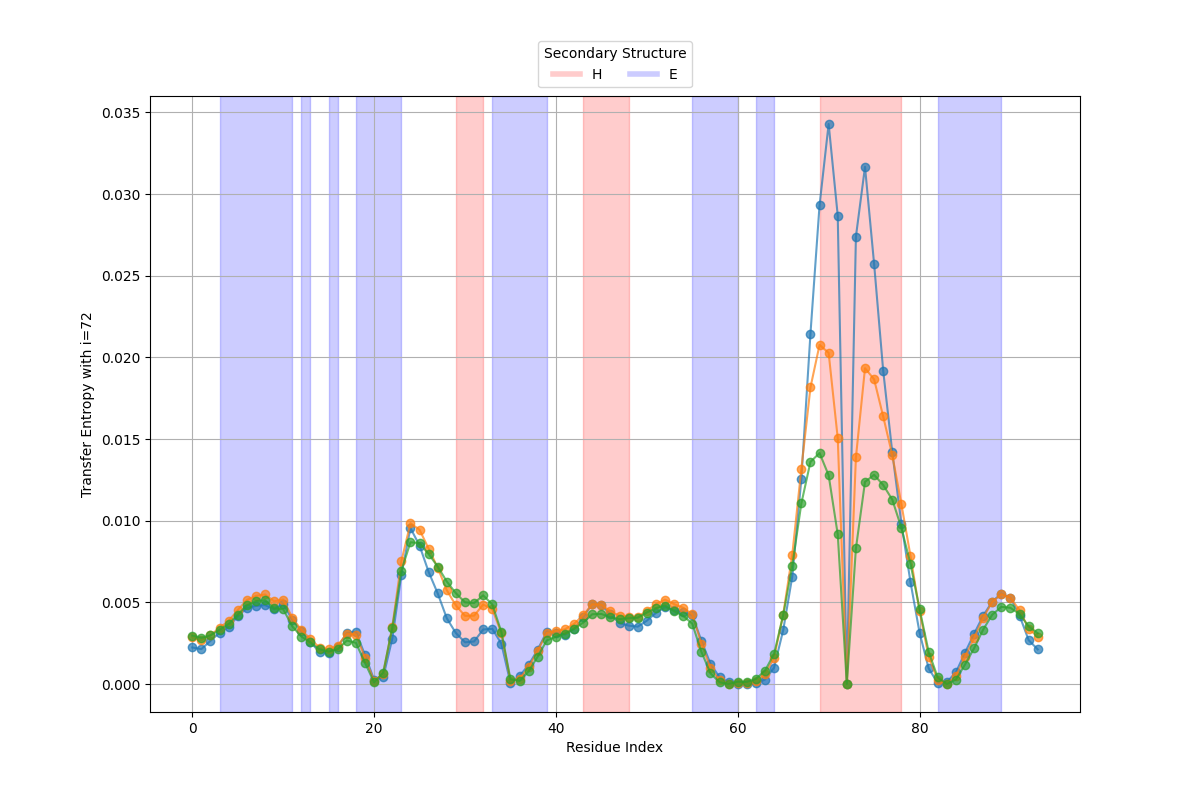
\includegraphics[width=0.8\textwidth]{/Users/enrico/PROTEINS/images/3LNX/Time_indicators/Transfer Entropy TE_ji for i=72 as a function of j at time index 0.png}
    \caption{Transfer Entropy 73->i (T_{i,73}).}
    \label{fig:TE73_pass}
\end{figure}

We can also analyze the vice versa transfer entropies obtaining the same results.\\



\newpage
\newpage

\newpage
\section{Conclusions of equlibrium stochastic process}
\noindent The analysis of residue correlations, dynamic responses, and transfer entropy not only provides a detailed description of internal dynamic interactions but also highlights critical elements of allostery and key residues that govern protein function.
These observations shed light on the functional interplay between the main secondary structural regions:  the binding pocket and the alpha helixs.
The analysis demonstrates that the geomtric strucutrue of the protein is so important that is sufficent to explain mathamically the allosteric propagation of the protein.\\
So this method can be used to predict the allosteric sites of a protein and to understand the mechanism of the protein, helping the experimental biologysts to stufy allostery.\\
In addition this analysis suggest that not only there is a comunication between allosteric sites and active sites in protein, but also there is a comunication between allosteric sites.\\


\newpage
\chapter{Out-of-Equilibrium Stochastic Processes Induced by Heat Gradients}
\noindent The first out-of-equilibrium condition for studying the protein is induced by a heat gradient.\\
In practice, what we will do is place the residues at two different temperatures based on their relative positions in the protein.\\
Infact it is imaginable that atoms inside the protein are more strongly bound and thus fluctuate less.\\
We introduced this heat gradient because we believe that allostery is often thought to emerge predominantly under non-equilibrium conditions.\\


\newpage
\section{Stochastic Dynamics Under a Heat Gradient}
\noindent In the equilibrium phase, as discussed in Chapter~\ref{sec:stochastic_processes}, the evolution of a system can be described by the following stochastic differential equation:
\begin{equation}
    \gamma \frac{dX_t}{dt} = -\nabla H(X_t) + \sqrt{2 \gamma k_B T} \eta_t.
\end{equation}

In a system subjected to a heat gradient, the temperature varies spatially across the protein structure, with each residue experiencing a local temperature \( T(x) \) that depends on its position.
This introduces a non-equilibrium condition driven by spatially dependent thermal fluctuations.\\ 
Consequently, the motion equation is modified to account for this temperature gradient:
\begin{equation}
    \gamma \frac{dX_t}{dt} = -\nabla H(X_t) + B \eta_t, \label{out_eq}
\end{equation}
where \( B \) is a diagonal matrix that incorporates the temperature of each residue. Specifically, \( B = \sqrt{2 \gamma k_B T(x)} \), making the noise term position-dependent.\\ 
For simplicity, let us assume the following parameter values:
\( \gamma = 1 \, \text{s}^{-1} \), \( k_B = 0.5 \, \text{J/K} \), and \( T(x) \) takes only two discrete values, representing two distinct thermal states.\\
Under these assumptions, the equation simplifies to:
\begin{equation}
    \frac{dX_t}{dt} = -K X_t + B \eta_t,
\end{equation}
where \( B \) is a diagonal matrix further refined to account for the discrete temperature values by incorporating a Kronecker delta function:\\
\begin{equation}
    B_{i,j} = \delta_{i,j} \cdot \sqrt{T(x)}.
\end{equation}
This model enables a detailed exploration of the stochastic dynamics of proteins under non-equilibrium conditions, offering a framework to quantify how spatial thermal gradients impact their structural and functional behavior.
\newpage
\section{Solution stochastic dynamics under a heat gradient}
We start from the original equation:
\[
\frac{dX_t}{dt} = -K X_t + B \eta_t.
\]
Substituting \(X_t = U Q_t\), we obtain:
\[
\frac{d(U Q_t)}{dt} = -K (U Q_t) + B \eta_t.
\]
Expanding the left-hand side:
\[
\frac{d(U Q_t)}{dt} = U \frac{dQ_t}{dt},
\]
because \(U\) is constant.\\
Substituting \(K = U \Lambda U^\top\), the term \(-K(U Q_t)\) becomes:
\[
-K(U Q_t) = -U \Lambda U^\top (U Q_t).
\]
Since \(U^\top U = I\) (orthogonality of \(U\)), the term simplifies to:
\[
- U \Lambda Q_t.
\]
The equation becomes:
\[
U \frac{dQ_t}{dt} = -U \Lambda Q_t + B \eta_t.
\]
Multiplying both sides by \(U^\top\) (to return to the eigenvector space):
\[
\frac{dQ_t}{dt} = -\Lambda Q_t + U^\top B \eta_t.
\]
We write this equation in components. For each component \(i\), we have:
\[
\frac{dQ_{i,t}}{dt} = -\lambda_i Q_{i,t} + \sum_j U_{ji}^\top B_{jj} \eta_{j,t}.
\]
The deterministic term \(-\lambda_i Q_{i,t}\) describes the evolution of the components \(Q_{i,t}\) under the influence of the eigenvalue \(\lambda_i\).\\
The stochastic term \(\sum_j U_{ji}^\top B_{jj} \eta_{j,t}\) represents the effect of noise transformed in the eigenvector space, with residual couplings arising from \(B\) and \(U\).\\
Now integrating both sides from \(-\infty\) to \(t\), we have:
\[
Q_{i,t} = \int_{-\infty}^t \left( -\lambda_i Q_{i,\tau} + \sum_j U_{ji}^\top B_{jj} \eta_{j,\tau} \right) d\tau.
\]
Using an integrating factor \(e^{\lambda_i t}\), the equation becomes:
\[
e^{\lambda_i t} Q_{i,t} = \int_{-\infty}^t e^{\lambda_i \tau} \sum_j U_{ji}^\top B_{jj} \eta_{j,\tau} \, d\tau.
\]
Simplifying, the solution is:
\[
Q_{i,t} = \int_{-\infty}^t e^{-\lambda_i (t - \tau)} \sum_j U_{ji}^\top B_{jj} \eta_{j,\tau} \, d\tau.
\]
We now compute the correlation:
\[
\langle Q_i(t) Q_j(s) \rangle = \left\langle \int_{-\infty}^t e^{-\lambda_i (t - \tau)} \sum_k U_{ki}^\top B_{kk} \eta_{k,\tau} \, d\tau \, \int_{-\infty}^s e^{-\lambda_j (s - \tau')} \sum_l U_{lj}^\top B_{ll} \eta_{l,\tau'} \, d\tau' \right\rangle.
\]
Expanding, we get:
\[
\langle Q_i(t) Q_j(s) \rangle = \int_{-\infty}^t \int_{-\infty}^s e^{-\lambda_i (t - \tau)} e^{-\lambda_j (s - \tau')} \sum_k \sum_l U_{ki}^\top B_{kk} U_{lj}^\top B_{ll} \langle \eta_{k,\tau} \eta_{l,\tau'} \rangle \, d\tau \, d\tau'.
\]
The noise term \(\langle \eta_{k,\tau} \eta_{l,\tau'} \rangle\) satisfies:
\[
\langle \eta_{k,\tau} \eta_{l,\tau'} \rangle = \delta_{kl} \delta(\tau - \tau'),
\]
which simplifies the double integral:
\[
\langle Q_i(t) Q_j(s) \rangle = \int_{-\infty}^{\min(t,s)} e^{-\lambda_i (t - \tau)} e^{-\lambda_j (s - \tau)} \sum_k (U_{ki}^\top B_{kk} U_{kj}^\top B_{kk}) \, d\tau.
\]
Factor out the exponential terms:
\[
\langle Q_i(t) Q_j(s) \rangle = \sum_k (U_{ki}^\top B_{kk}) (U_{kj}^\top B_{kk}) \int_{-\infty}^{\min(t,s)} e^{-\lambda_i (t - \tau)} e^{-\lambda_j (s - \tau)} \, d\tau.
\]
Simplify the exponential combination:
\[
e^{-\lambda_i (t - \tau)} e^{-\lambda_j (s - \tau)} = e^{-(\lambda_i t + \lambda_j s)} e^{(\lambda_i + \lambda_j) \tau}.
\]
The integral becomes:
\[
\int_{-\infty}^{\min(t,s)} e^{-(\lambda_i t + \lambda_j s)} e^{(\lambda_i + \lambda_j) \tau} \, d\tau.
\]
Evaluating the integral:
\[
\int_{-\infty}^{\min(t,s)} e^{-(\lambda_i t + \lambda_j s)} e^{(\lambda_i + \lambda_j) \tau} \, d\tau = \frac{e^{-(\lambda_i t + \lambda_j s)}}{\lambda_i + \lambda_j} \left[ e^{(\lambda_i + \lambda_j) \min(t,s)} \right].
\]
Substitute back:
\[
\langle Q_i(t) Q_j(s) \rangle = \sum_k \frac{(U_{ki}^\top B_{kk}) (U_{kj}^\top B_{kk})}{\lambda_i + \lambda_j} e^{-\lambda_i t - \lambda_j s} \left( e^{(\lambda_i + \lambda_j) \min(t,s)} \right).
\]
Simplify further:
\[
\langle Q_i(t) Q_j(s) \rangle = \sum_k \frac{(U_{ki}^\top B_{kk}) (U_{kj}^\top B_{kk})}{\lambda_i + \lambda_j} e^{-\lambda_i |t-s|}.
\]
So:
\[
\langle X_i(t) X_j^\top(s) \rangle = \sum_k \sum_p \sum_m \frac{U_{ik} U_{jp} (U_{mk}^\top B_{mm}^2 U_{mp}^\top)}{\lambda_k + \lambda_p} e^{-\lambda_k |t-s|}.
\]
The formula describes the temporal correlation between the components \( X_i(t) \) and \( X_j(s) \) in a stochastic system under the influence of noise. Each term in the formula has a specific role, in fact, the coupling through Eigenvectors (\( U_{ik} \) and \( U_{jp} \)) project the system's dynamics into the eigenbasis of the matrix \( \mathbf{K} \), capturing how the eigenmodes contribute to the observed correlations between \( i \) and \( j \), the diagonal matrix \( B_{mm}^2 \) introduces temperature-dependent scaling of the stochastic noise.\\
This reflects the local intensity of fluctuations at mode \( m \), the product of \( U_{mk}^\top \) and \( U_{mp}^\top \) determines how noise from mode \( m \) couples different eigenmodes \( k \) and \( p \), weighted by the structure of the eigenvectors, the term \( e^{-\lambda_k |t-s|} \) encapsulates the temporal decay of the correlation, governed by the eigenvalue \( \lambda_k \).\\ 
Larger eigenvalues correspond to faster decay, indicating less persistent correlations over time.
The denominator ensures that the contributions from eigenmodes are properly weighted by their respective damping rates \( \lambda_k \) and \( \lambda_p \), balancing the dynamic interactions between modes.

As before the transfer entropy it is completely determined by the correlation.
Otherwise define the linear response out of equilibrium is not possible.


\newpage
\section{Temperature determination}
\noindent As we said, we set two distinct temperature regimes.\\
One temperature is fixed at \( T = 1 \), representing a high-energy state, while the other temperature varies between \( T = 0 \) and \( T = 1 \) for each experiment, so it is \( T = 1 - \epsilon,\),
where \( \epsilon = \{1.0, 0.9, 0.8, 0.7, 0.6, 0.5, 0.4, 0.3, 0.2, 0.1, 0.0\} \) for a total of 11 experiments (Note that when  \( epsilon = 0 \) we are in the equilibrium case as before, so the results must be the same).\\
This configuration allows us to drive the system out of equilibrium and study the allosteric behavior under non-equilibrium conditions.\\
The temperature assigned to a given residue is determined based on its connectivity within the protein structure. Specifically, if a residue has five or more connections, it is assigned a temperature of \( T = 1 - \epsilon,\)  (varying temperature);
otherwise, it is assigned \( T = 1 \). This methodology links the temperature directly to the residue's position and role within the protein network.

Residues located near the center of the protein typically exhibit a higher number of connections due to their central role in maintaining structural integrity. These residues tend to fluctuate less and are therefore associated with lower effective temperatures. Conversely, residues with fewer connections, often found on the periphery, are more flexible and are assigned higher temperatures.\\
By combining fixed and variable temperature conditions, this approach enables a deeper understanding of the relationship between protein topology, residue connectivity, and dynamic behavior under non-equilibrium states. The differential temperature settings also provide a framework to explore how structural positions influence allosteric signaling and energy distribution across the protein.\\
\begin{figure}[h!]
    \centering
    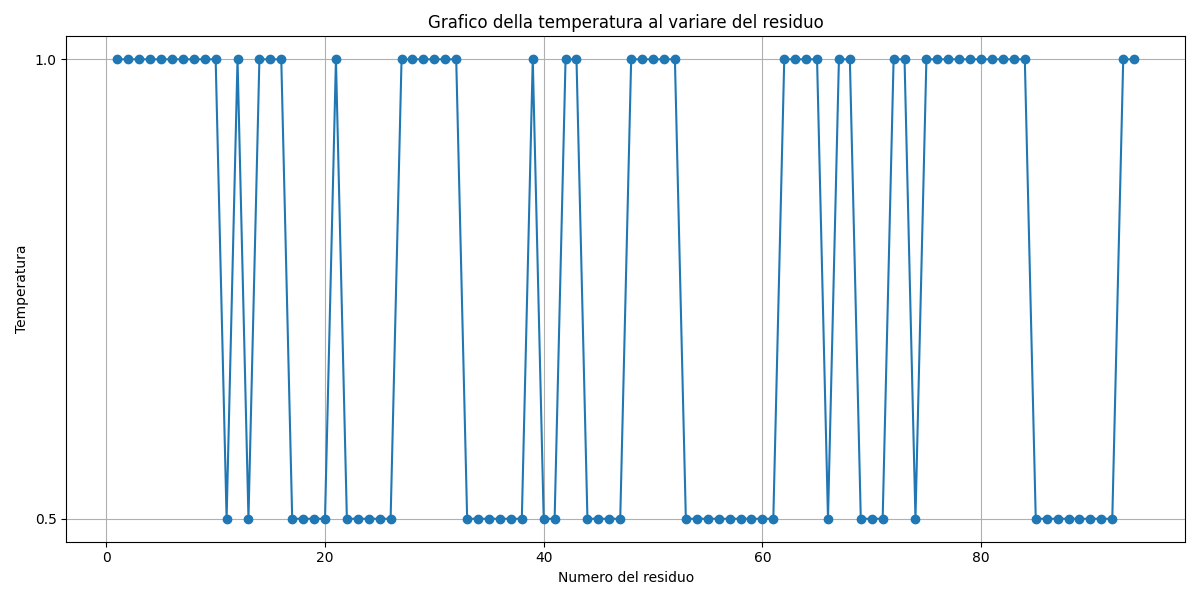
\includegraphics[width=0.8\textwidth]{/Users/enrico/PROTEINS/images/3LNX/2_temperature_cutoff/temperatures.png}
    \caption{Temperature vs residue number}
\end{figure}
What we can see is that in the beta sheet regions residues tend to have higher connectivity due to their compact and stabilizing arrangement in the protein's core, otherwhise in the Alpha helix regions typically exhibit intermediate levels of connectivity.\\
Finally residues located in loops or on the protein's surface generally have fewer connections, as these regions are more exposed and less structurally integrated.
This lower connectivity results in higher assigned temperatures

\newpage
\chapter{Experimental results non equilibrium dynamic}
In this chapter we will expose the reseults obtain for the non-equilibrium stochastic process describing the oscilaltions of atoms in the protein under a heat gradient.\\
For the connection radius and for the Kirchhoff matrix are valid the precedence arguments respectively in sections \ref{connection_radius} and \ref{Kirchhoff_paragraph}.\\
In addition we used the same characteristic time finded in the equilibrium case: .\\
\section{Correlation Matrix}
\noindent 
The two figures illustrate the correlation matrices obtained from the protein structure. The elements of the matrix represent correlations between residues \(i\) and \(j\), derived from the dynamics and structure of the system.\\
Overlaying the secondary structure (Helices: red; Beta Sheets: blue) helps to contextualize the correlations within structural motifs. The Kirchhoff matrix was used to compute these correlations.
\begin{figure}[h!]
    \centering
    \begin{minipage}{0.49\textwidth}
        \centering
        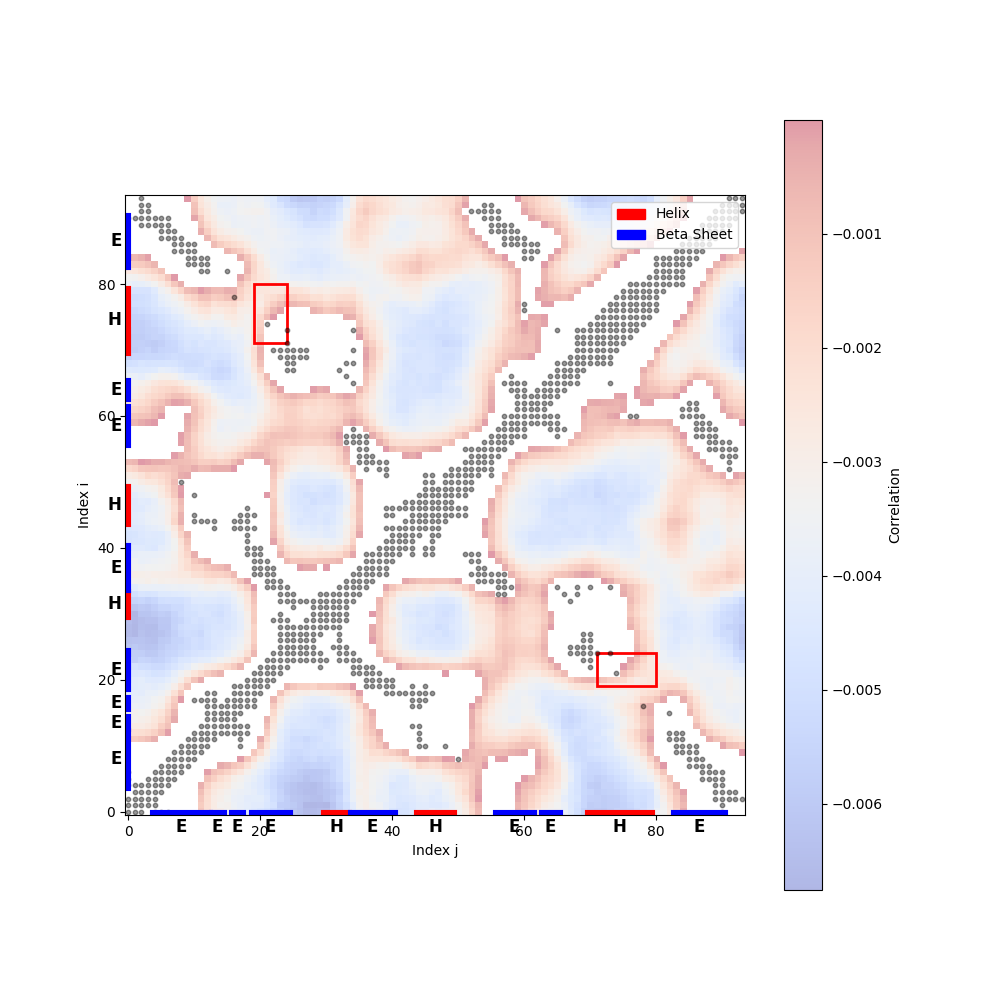
\includegraphics[width=\textwidth]{/Users/enrico/PROTEINS/images/3LNX/2_temperature_cutoff/Matrici_Correlazione/Correlation_MatrixNan_False_0.5.png}
        \caption{Negative covariance between residues at time 0 with $max \Delta T = 0.5$.}
    \end{minipage}
    \hfill
    \begin{minipage}{0.49\textwidth}
        \centering
        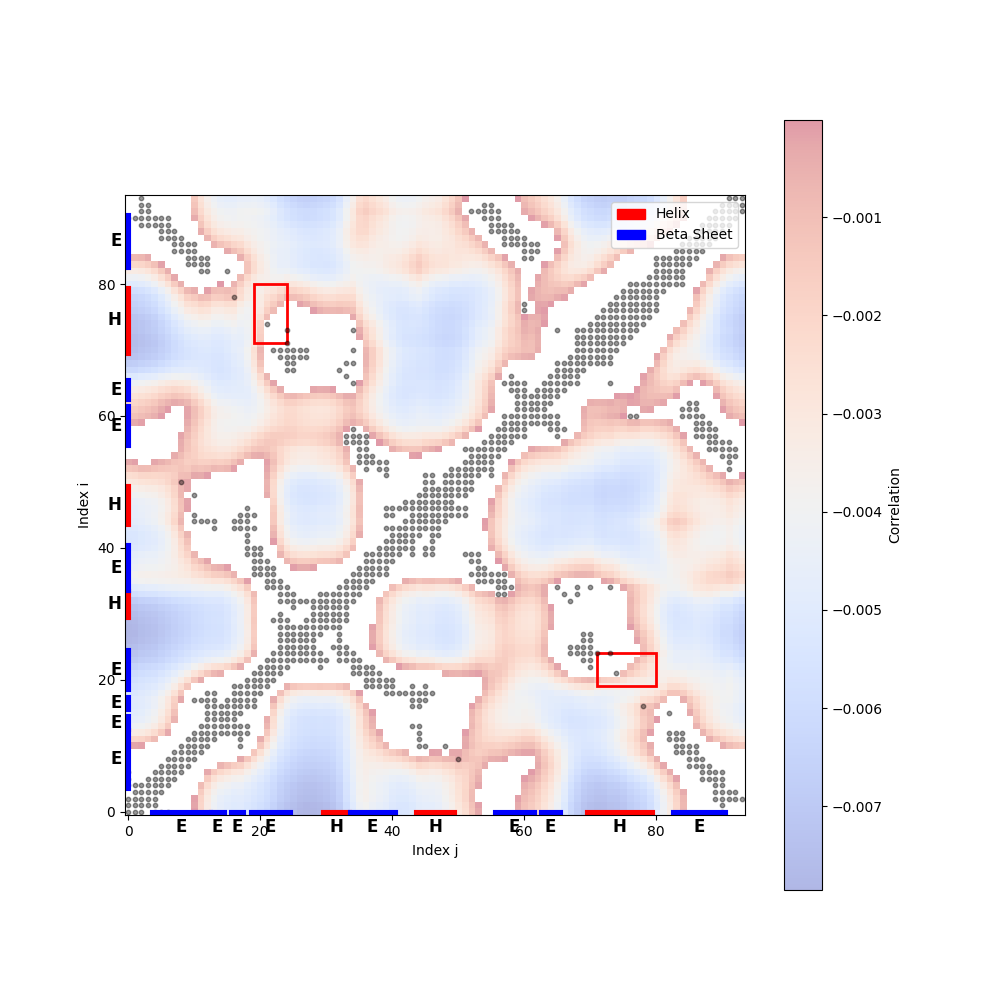
\includegraphics[width=\textwidth]{/Users/enrico/PROTEINS/images/3LNX/2_temperature_cutoff/Matrici_Correlazione/Correlation_MatrixNan_False_1.png}
        \caption{Negative covariance between residues at time 0 with $max \Delta T = 1$.}
    \end{minipage}
    \caption{Comparison of negative covariances between residues at time 0 for different $max \Delta T$ values.}
    \label{fig:correlation_comparison_out}

\end{figure}


\begin{figure}[h!]
    \centering
    \begin{minipage}{0.49\textwidth}
        \centering
        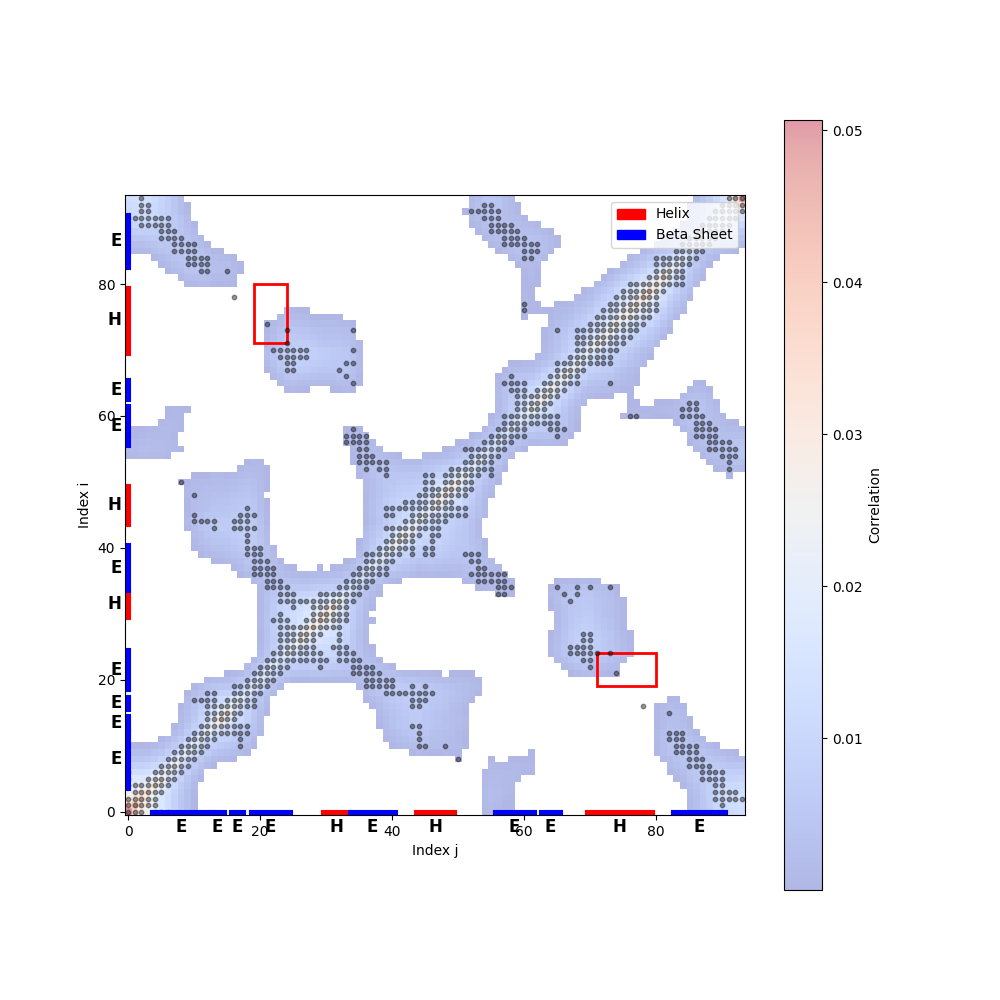
\includegraphics[width=\textwidth]{/Users/enrico/PROTEINS/images/3LNX/2_temperature_cutoff/Matrici_Correlazione/Correlation_MatrixNan_True_0.5.png}
        \caption{Positive covariance between residues at time 0 with $max \Delta T = 0.5$.}
        
    \end{minipage}
    \hfill
    \begin{minipage}{0.49\textwidth}
        \centering
        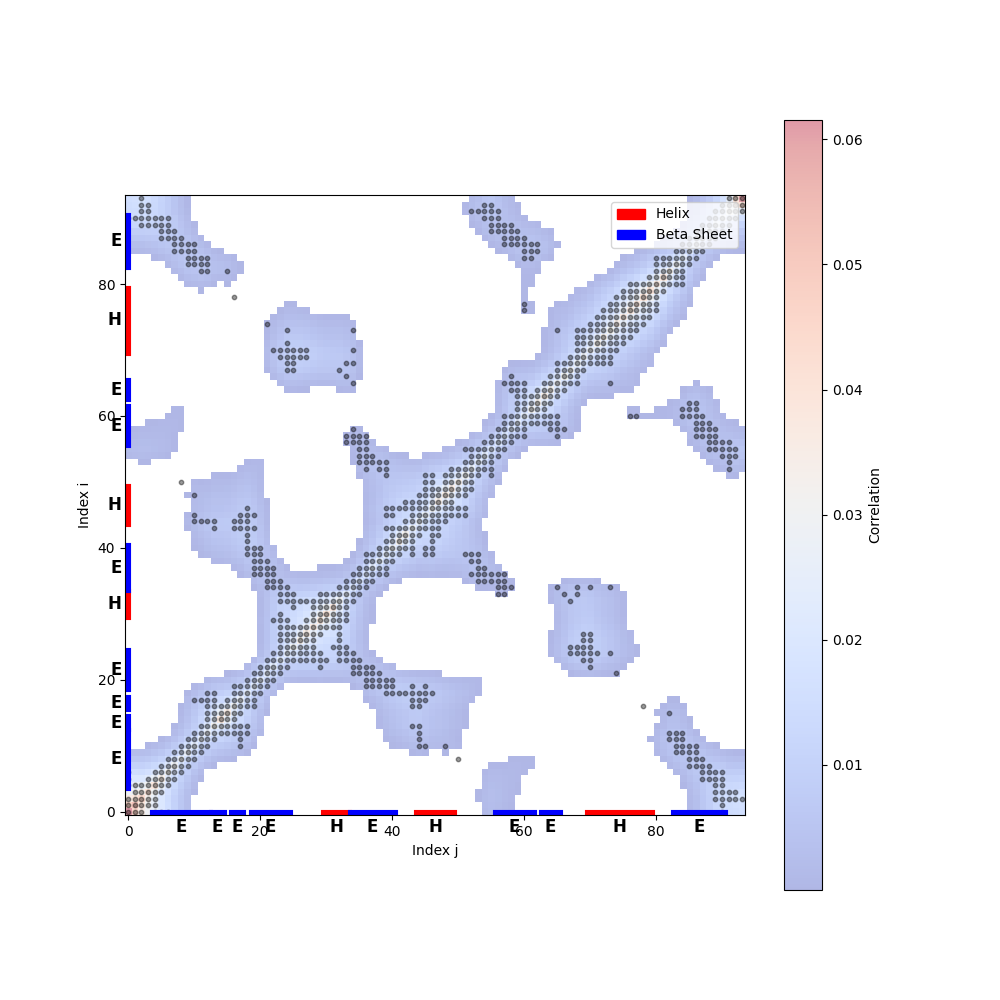
\includegraphics[width=\textwidth]{/Users/enrico/PROTEINS/images/3LNX/2_temperature_cutoff/Matrici_Correlazione/Correlation_MatrixNan_True_1.png}
        \caption{Positive covariance between residues at time 0 with $max \Delta T = 1$.}
        
    \end{minipage}
    \caption{Comparison of positive covariances between residues at time 0 for different $max \Delta T$ values.}
    \label{fig:correlation_positive_comparison_out}
\end{figure}



In the image \ref{fig:correlation_comparison_out} it is represents the negative part of the correlation matrix at two different temperature.\\
The left matrix (\(max \Delta T = 0.5\)) shows finer structural detail with localized negative covariance patterns, particularly within the secondary structure regions.\\
Instead the right matrix (\(max \Delta T = 1\)) exhibits smoother covariance patterns, possibly due to increased flexibility or averaging effects with a higher temperature range.\\
Differences between the two matrices emphasize how temperature cutoffs influence residue correlation patterns and reflect the sensitivity of structural motifs to dynamic conditions.

Instead the image \ref{fig:correlation_positive_comparison_out} it is represents the positive part of the correlation matrix at two different temperature.\\
At \(max \Delta T = 0.5\), the correlation patterns are more localized, capturing finer structural detail and tighter residue coupling.\\
At \(max \Delta T = 1\), the correlations are more diffuse, suggesting increased flexibility or dynamic averaging effects.\\
The comparison highlights how increasing the temperature cutoff alters the correlation landscape, reflecting changes in the dynamic behavior of the protein.

\newpage
\newpage




\section{Beta Factors}
\noindent The plot above compares the experimental \( B \)-factors (blue curve), where \eqref{beta} $B_i = 8\pi^2 C_{ii}$, with the predicted \( B \)-factors (red curve) along the residue index. 

These metrics provide a quantitative assessment of the model's accuracy in capturing the protein's dynamic behavior.
\begin{table}[ht]
    \centering
    \begin{tabular}{|c|c|c|}
        \hline
        $\Delta T$ & MAE & RMSE \\ \hline
        $T=1$ & 6.4146 &  8.5200 \\ \hline
        $T=0.9$ & 6.3206 &  8.4244 \\ \hline
        $T=0.8$ & 6.2239 &  8.3239 \\ \hline
        $T=0.7$ & 6.1239 &  8.2191 \\ \hline
        $T=0.6$ & 6.0212 &  8.1107\\ \hline
        $T=0.5$ & 5.9457 &  8.0004 \\ \hline
        $T=0.4$ & 5.8701 &  7.8913 \\ \hline
        $T=0.3$ & 5.8117 &  7.7885 \\ \hline
        $T=0.2$ & 5.7542 &  7.7003 \\ \hline
        $T=0.1$ & 5.7030 &  7.6413 \\ \hline
        $T=0.0$ & 5.6775 &  7.6349 \\ \hline
    \end{tabular}
    \caption{Errors of MAE and RMSE for different values of $\Delta T$}
    \label{tab:mae_rmse}
\end{table}


\begin{figure}[h!]
    \centering
    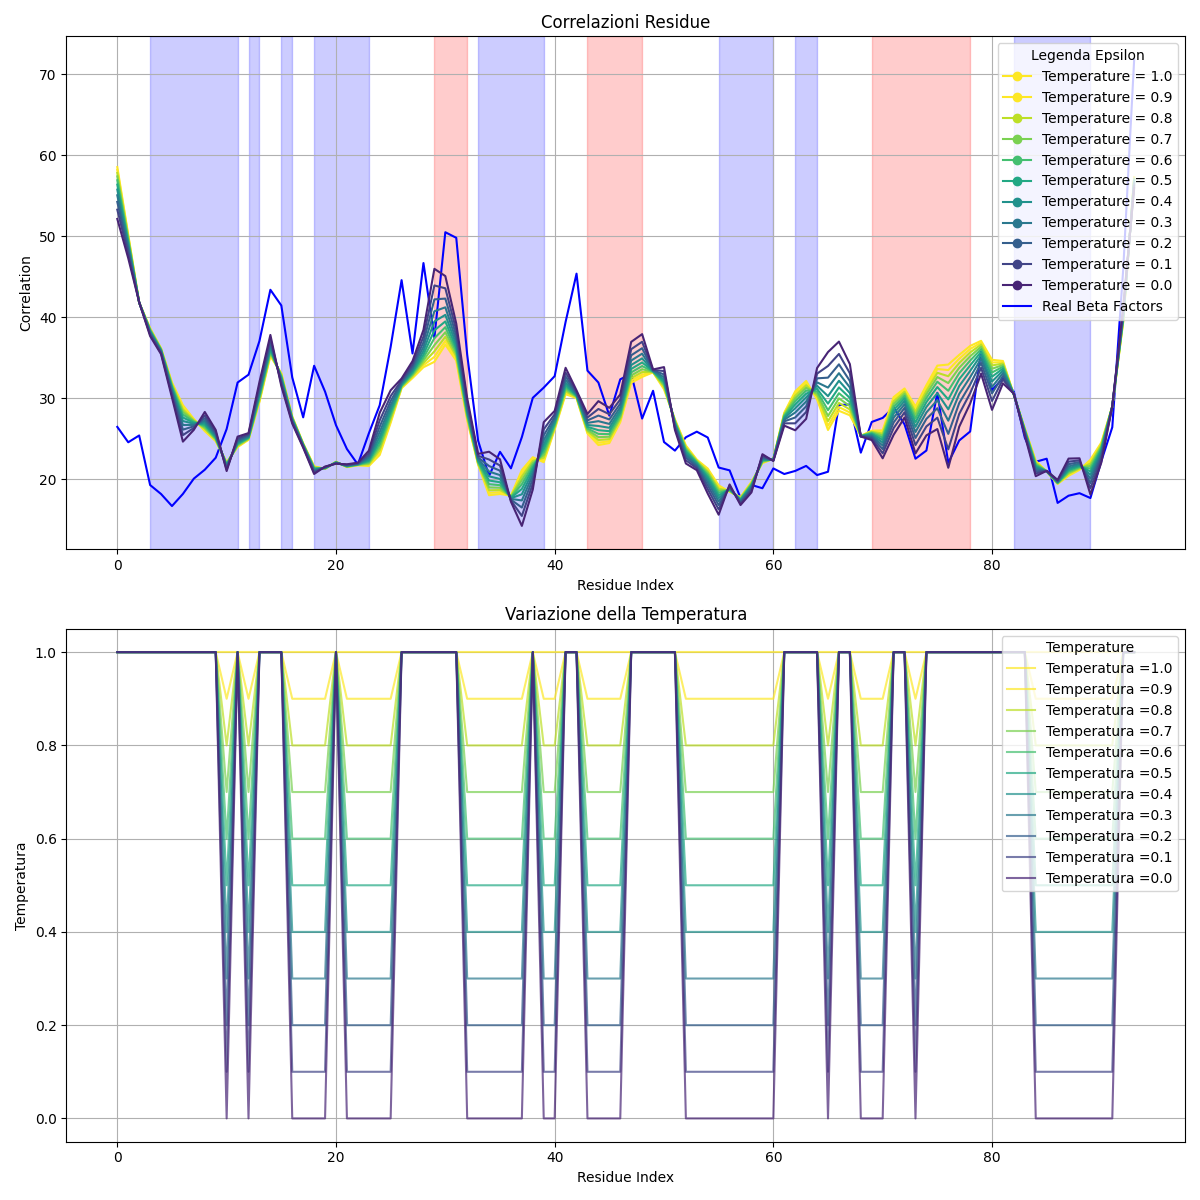
\includegraphics[width=0.8\textwidth]{/Users/enrico/PROTEINS/images/3LNX/2_temperature_cutoff/beta_factors/beta.png}
    \caption{Beta factors with different $\Delta T$.}
\end{figure}


The results showcase how varying the applied temperature difference (\(\Delta T\)) affects the predictive accuracy of \( B \)-factors, which represent atomic displacement or flexibility of residues in the protein structure. \\
The blue curve represents the experimental \( B \)-factors, and the red curve represents the predicted values:
The predicted \( B \)-factors align closely with the experimental values across much of the residue index, suggesting that the system's response to a larger temperature gradient is more structured and predictable.

By analyzing \(\Delta T = 1\) and \(\Delta T = 1 - \epsilon \), we observe that the system driven out of equilibrium (\(\Delta T = 1\)) exhibits more predictable dynamics, resulting in lower error metrics and better alignment between predicted and experimental \( B \)-factors. \\
In the bottom plot as before there are the different temperatures.\\

These findings highlight an important principle: systems driven out of equilibrium exhibit more structured and predictable behavior. 

\newpage
\section{Causal indicators in time}
\noindent Now we will see the cross covariance in time and the transfer entropy in time.\\
We will attend a non simmetric funcitonal form backward and forward.



\subsection{Cross covariance in time}
\begin{figure}[h!]
    \centering
    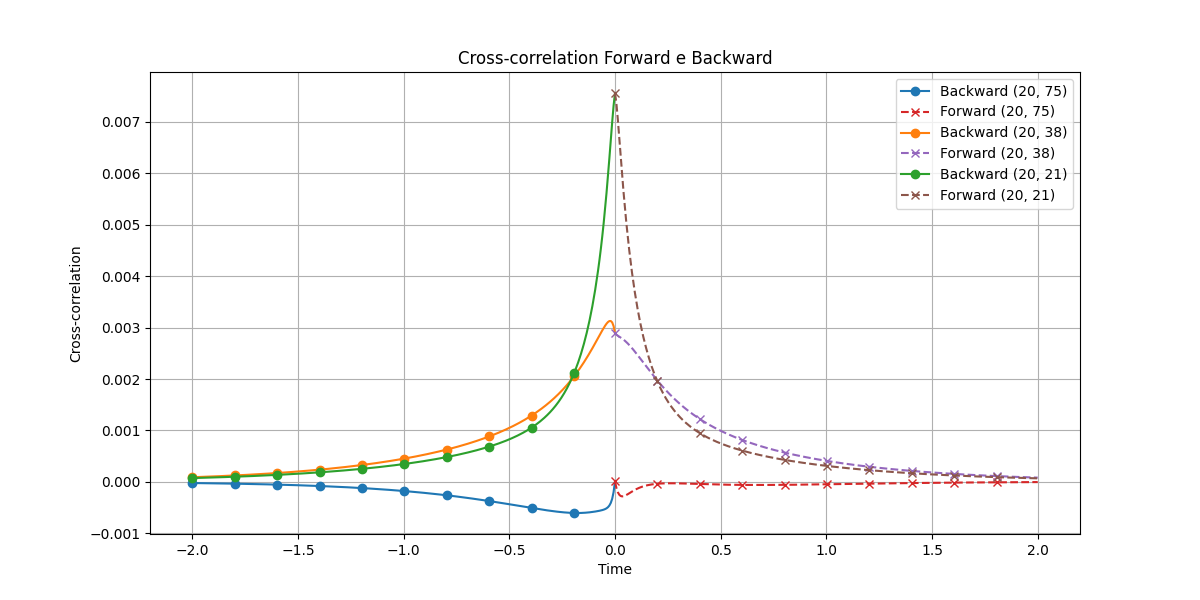
\includegraphics[width=0.8\textwidth]{/Users/enrico/PROTEINS/images/3LNX/2_temperature_cutoff/Time_correlations/correlation_combined.png}
    \caption{Correlation in time $\Delta T = 1$.}
\end{figure}
\noindent  Let’s start with the covariance in time, as we said before the correlation is defined
as:
\[
\langle X_i(t) X_j^\top(s) \rangle = \sum_k \sum_p \sum_m \frac{U_{ik} U_{jp} (U_{mk}^\top B_{mm}^2 U_{mp}^\top)}{\lambda_k + \lambda_p} e^{-\lambda_k |t-s|}.
\]
This behavior is coherent with what expected, the correlation decay over time,indicating a loss of direct dynamic influence as time progresses.
Moreover correlation values vary significantly between residue pairs, reflecting
differences in their initial dynamic coupling.\\
In additon out of equilibrium we can see that the cross-covariance is not time simmetric, in fact the forward covaraince is different from the backward.\\

\newpage
\subsection{Transfer Entropy: Forward and Backward Dynamics}
\begin{figure}[h!]
    \centering
    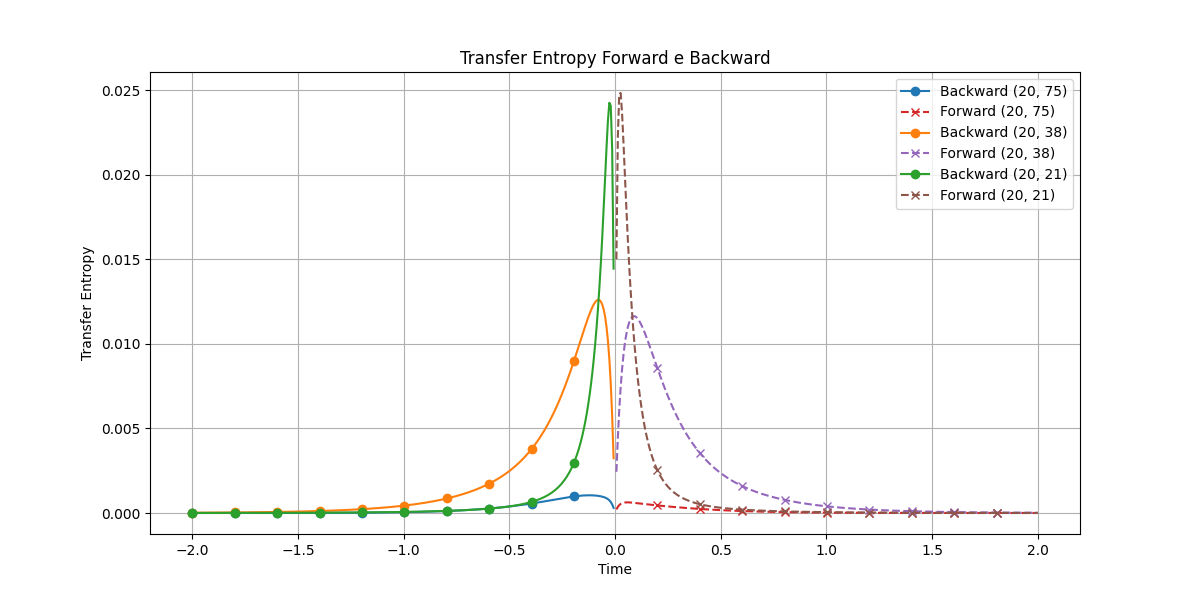
\includegraphics[width=0.8\textwidth]{/Users/enrico/PROTEINS/images/3LNX/2_temperature_cutoff/Time_correlations/entropies_combined.png}
    \caption{Transfer entropy in time $\Delta T = 1$.}
\end{figure}

\noindent Also here, Obviosly, the transfer entropy is not time simmetric.\\
In addition the equilibrium reaseasons are valid: We see that a peak is observed at an intermediate time point for
most residue pairs, indicating a time of maximum information transfer.

\newpage
\section{Causal indicators between residues}
\newpage
\subsection{Correlation between residues}
\noindent 
In the following figures, we will analyze the covariance between residues.\\
We want to see, as before, a high absolute value of covariance between the allosteric sites and the active sites in the binding pocket.\\

\begin{figure}[h!]
    \centering
    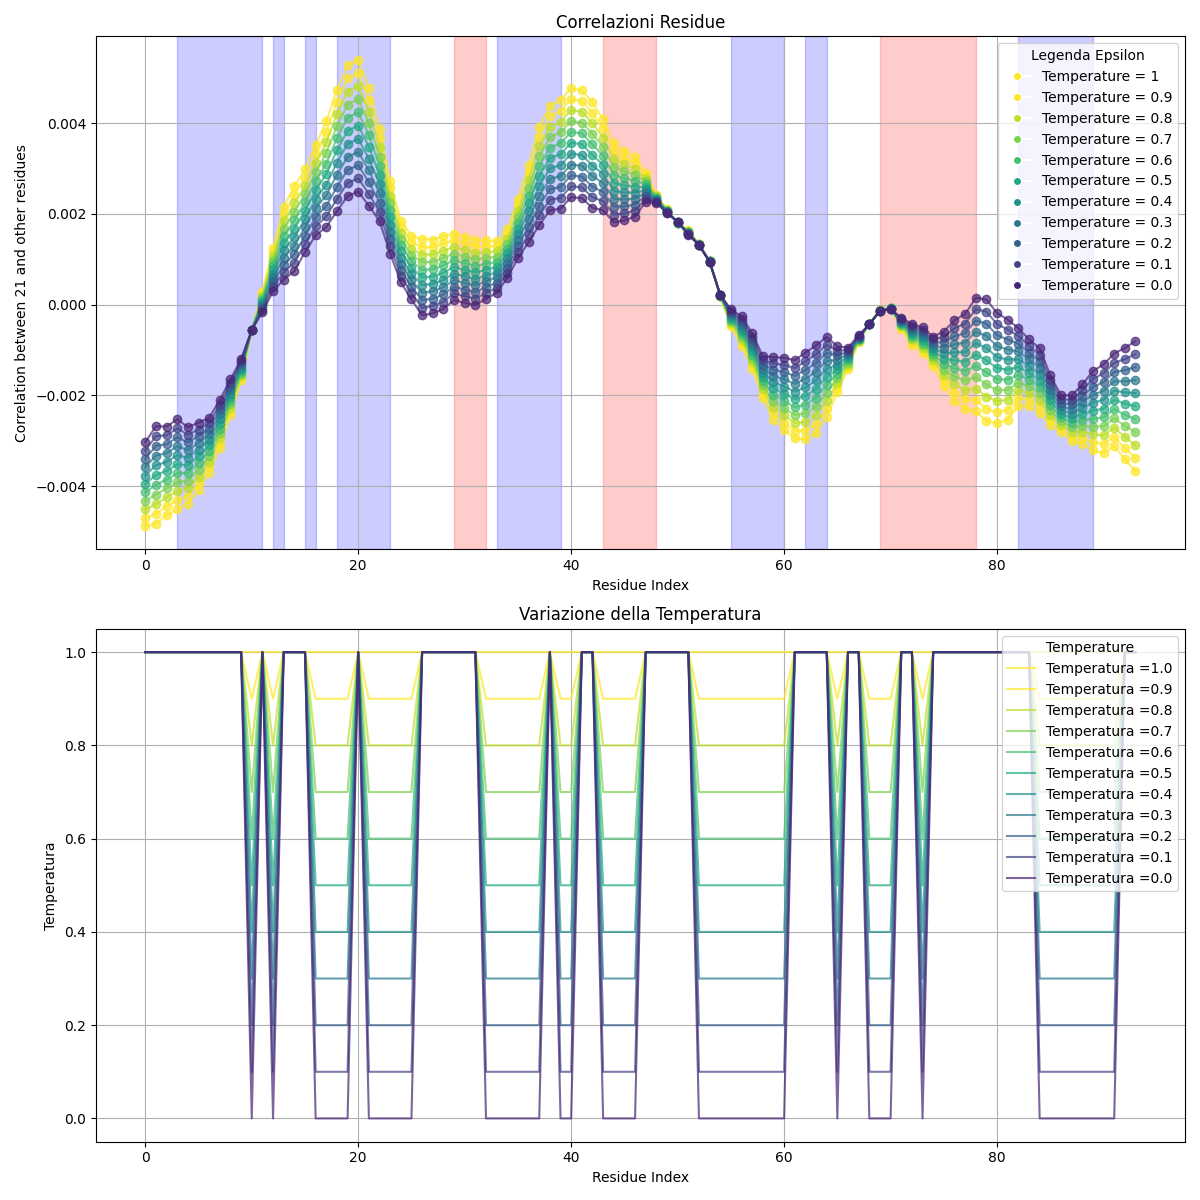
\includegraphics[width=0.8\textwidth]{/Users/enrico/PROTEINS/images/3LNX/2_temperature_cutoff/combined_correlation_20_temperature_plots.png}
    \caption{Correlation perturbating 21-th residue.}
    \label{fig:corr21_out}
\end{figure}
\begin{figure}[h!]
    \centering
    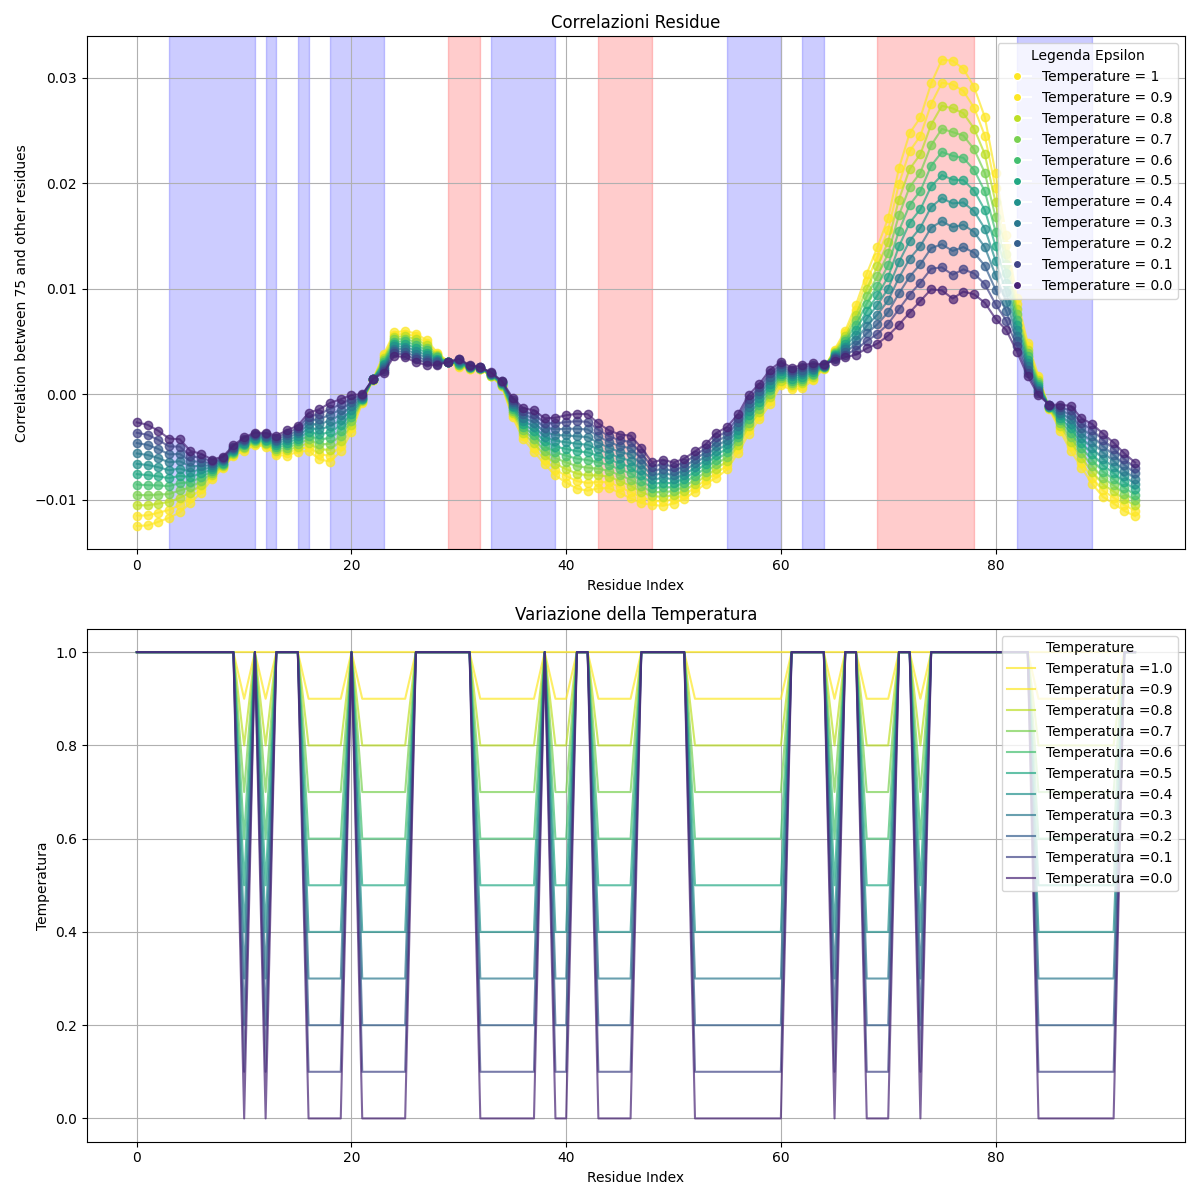
\includegraphics[width=0.8\textwidth]{/Users/enrico/PROTEINS/CUTOFF/images/3LNX/2_temperature_cutoff/combined_correlation_75_temperature_plots.png}
    \caption{Correlation perturbating 76-th residue.}
    \label{fig:corr76_out}
\end{figure}
When temperatures are higher we can see how more dispersed and higher in modulus the correlation are.\\
Instead at lower temperatures the correlation are more localized.\\
We can alsoo see that the covariance for some residues are completely indifferent to the heat gradient.\\ 

\subsubsection{Temperature Variation and General Observations}
\begin{itemize}
    \item \textbf{Temperature Oscillations:} Both figures show regular oscillations in temperature, reflecting dynamic structural changes in the protein.
    \item \textbf{Flexibility vs. Rigidity:} High temperatures (\( T = 1.0 \)) are associated with broader fluctuations and more dispersed correlation effects, while low temperatures (\( T = 0.0 \)) correspond to sharp, localized peaks, indicating more rigid and limited dynamic behavior.
\end{itemize}

\subsubsection{Conclusions}
\begin{itemize}
    \item The temperature significantly affects the flexibility and dynamics of residue correlations.
    \item Residues 76 and 21 represent dynamically significant points in the protein structure, with residue 76 showing greater dynamic influence overall.
    \item These results suggest that thermal regulation could be a critical mechanism for modulating the structural and functional dynamics of the protein.
\end{itemize}









\newpage
\newpage


\begin{figure}[htbp]
    \centering
    % Prima sottografia
    \begin{subfigure}[t]{0.45\textwidth}
        \centering
        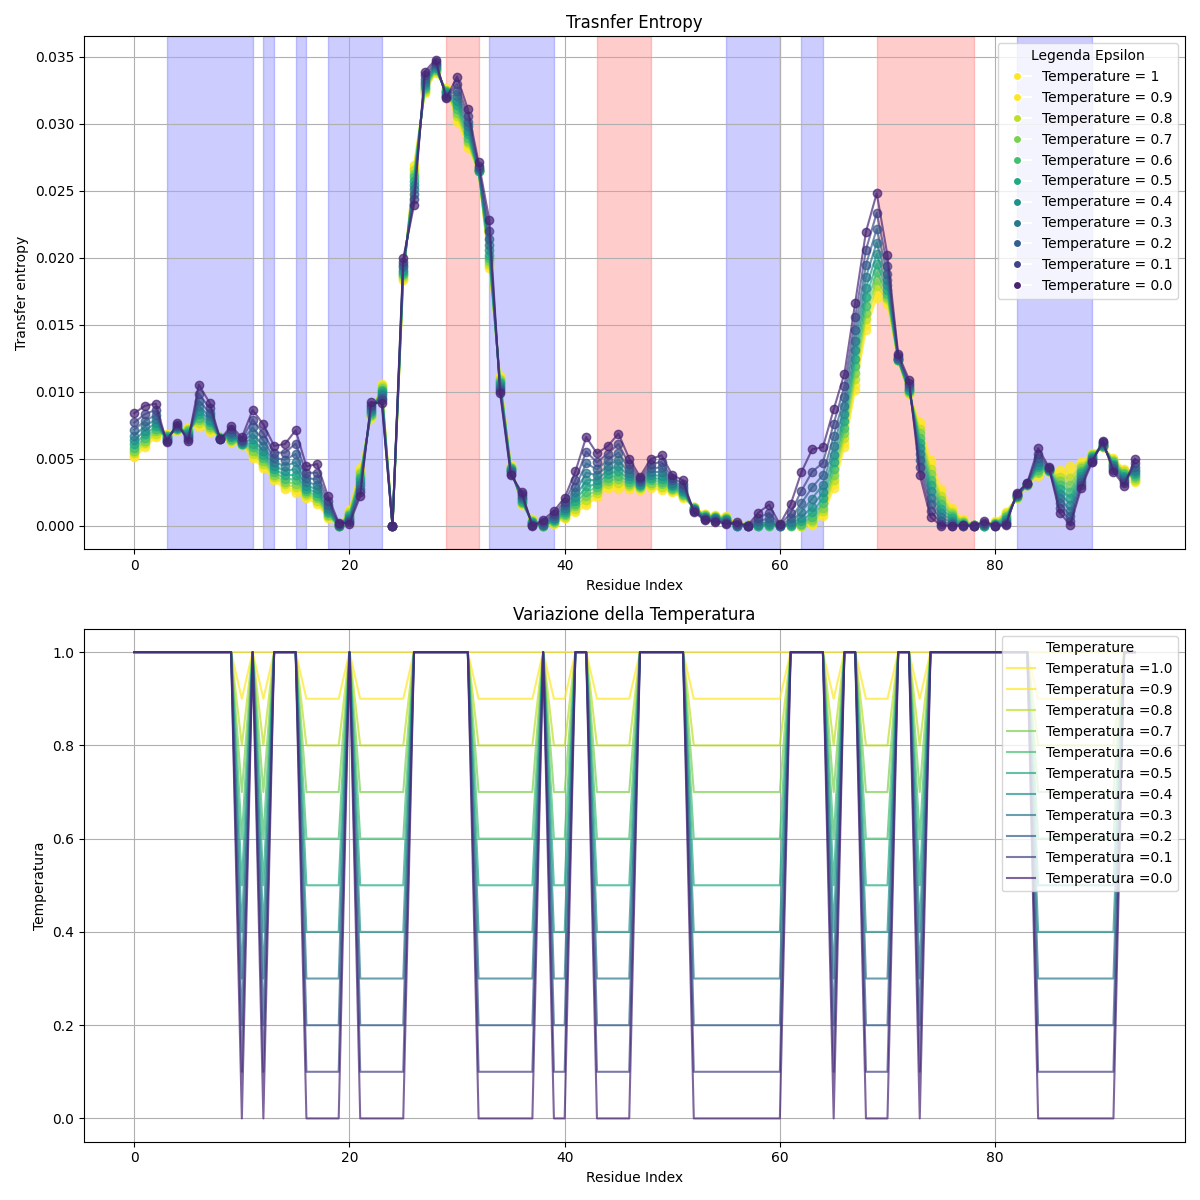
\includegraphics[width=\textwidth]{/Users/enrico/PROTEINS/CUTOFF/images/3LNX/2_temperature_cutoff/combined_entropy_temperature_20_plots.png}
        \caption{Transfer Entropy ($TE_{21,j}$) perturbating the 21st residue.}
        \label{fig:TE21_i_j_out}
    \end{subfigure}
    \hfill
    % Seconda sottografia
    \begin{subfigure}[t]{0.45\textwidth}
        \centering
        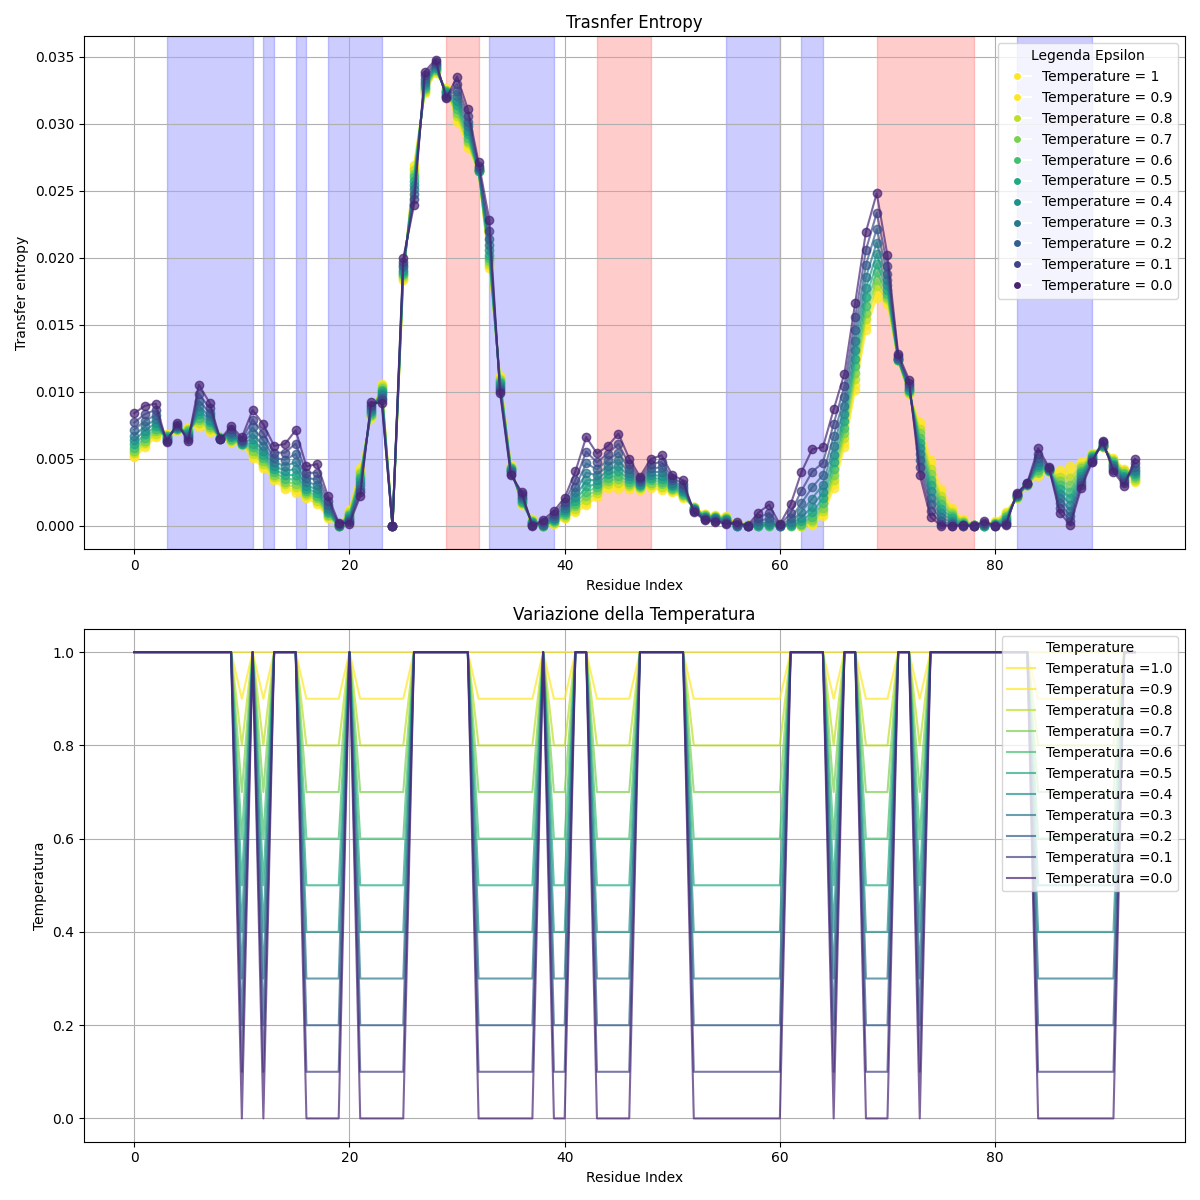
\includegraphics[width=\textwidth]{/Users/enrico/PROTEINS/CUTOFF/images/3LNX/2_temperature_cutoff/combined_entropy_temperature_75_plots.png}
        \caption{Transfer Entropy ($TE_{76,j}$) perturbating the 76th residue.}
        \label{fig:TE76_i_j_out}
    \end{subfigure}
    % Didascalia principale
    \caption{Comparison of Transfer Entropy for different perturbed residues.}
    \label{fig:TE_comparison_i_j_out}
\end{figure}


\subsection{Conclusion}
The analysis reveals that driving the system out of equilibrium (\(\Delta T = 1\)) results in lower MAE and RMSE values and better alignment between predicted and experimental \( B \)-factors. Non-equilibrium conditions create more structured and predictable dynamics, while closer-to-equilibrium systems (\(\Delta T = 0.5\)) exhibit subtler and more stochastic flexibility patterns. These findings underscore the stabilizing effect of non-equilibrium conditions on protein dynamics and highlight the critical role of temperature gradients in studying and modeling protein flexibility.


\newpage
\newpage
\begin{thebibliography}{100}

    \bibitem{ref} 
    \url{https://www.sciencelearn.org.nz/resources/209-role-of-proteins-in-the-body}
    
    \bibitem{ref2} 
    \emph{University of California Davis, Introductory Biology}, 
    \url{https://bio.libretexts.org/Courses/University_of_California_Davis/BIS_2A%3A_Introductory_Biology_%28Easlon%29/Readings/04.3%3A_Amino_Acids}
    
    \bibitem{ref3} 
    \emph{University of California Davis, Introductory Biology}, 
    \url{https://bio.libretexts.org/Courses/University_of_California_Davis/BIS_2A%3A_Introductory_Biology_%28Britt%29/01%3A_Readings/1.17%3A_Protein_Structure}
    
    \bibitem{ref4} 
    Nature, \url{https://www.nature.com/scitable/topicpage/protein-structure-14122136/}
    
    \bibitem{ref5} 
    Wikipedia, Allosteric regulation 
    
    \bibitem{ref6} 
    Statistical Mechanics of Allosteric Enzymes
    
    \bibitem{ref7} 
    University of California Davis, Introductory Biology, Hemoglobin and allosteric effects
    
    \bibitem{ref8} 
    Allosterism in the PDZ Family, Amy O. Stevens and Yi He
    
    \bibitem{ref9} 
    Protein elastic network models and the ranges of cooperativity, Lei Yanga, Guang Songa, and Robert L. Jernigana
    
    \bibitem{ref11} 
    Introduzione alla Teoria dei Grafi, Vittorio Loreto, Francesca Tria.
    
    \bibitem{ref12} 
    Time and ensemble-average statistical mechanics of the Gaussian network model, Alessio Lapolla, Maximilian Vossel, and Aljaz Godec
    
    \bibitem{ref13} 
    Correlation, response and entropy approaches to allosteric behaviors: a critical comparison on the ubiquitin case Fabio Cecconi, Giulio constantini, Carlo Guardiani, Marco Baldovin and Angelo Vulpiani
    
    \bibitem{ref14} 
    Robust inference of causality in high-dimensional dynamical processes from the Information Imbalance of distance ranks
    Vittorio Del Tatto, Gianfranco Fortunato, Domenica Bueti, and Alessandro Laio
    
    \bibitem{ref15} 
    Allosterism in the PDZ Family, Amy O. Stevens and Yi He.

    
\end{thebibliography}

\end{document}
